% Template for PLoS
% Version 3.5 March 2018
%
% % % % % % % % % % % % % % % % % % % % % %
%
% -- IMPORTANT NOTE
%
% This template contains comments intended 
% to minimize problems and delays during our production 
% process. Please follow the template instructions
% whenever possible.
%
% % % % % % % % % % % % % % % % % % % % % % % 
%
% Once your paper is accepted for publication, 
% PLEASE REMOVE ALL TRACKED CHANGES in this file 
% and leave only the final text of your manuscript. 
% PLOS recommends the use of latexdiff to track changes during review, as this will help to maintain a clean tex file.
% Visit https://www.ctan.org/pkg/latexdiff?lang=en for info or contact us at latex@plos.org.
%
%
% There are no restrictions on package use within the LaTeX files except that 
% no packages listed in the template may be deleted.
%
% Please do not include colors or graphics in the text.
%
% The manuscript LaTeX source should be contained within a single file (do not use \input, \externaldocument, or similar commands).
%
% % % % % % % % % % % % % % % % % % % % % % %
%
% -- FIGURES AND TABLES
%
% Please include tables/figure captions directly after the paragraph where they are first cited in the text.
%
% DO NOT INCLUDE GRAPHICS IN YOUR MANUSCRIPT
% - Figures should be up\textit{loaded} separately from your manuscript file. 
% - Figures generated using LaTeX should be extracted and removed from the PDF before submission. 
% - Figures containing multiple panels/subfigures must be combined into one image file before submission.
% For figure citations, please use "Fig" instead of "Figure".
% See http://journals.plos.org/plosone/s/figures for PLOS figure guidelines.
%
% Tables should be cell-based and may not contain:
% - spacing/line breaks within cells to alter layout or alignment
% - do not nest tabular environments (no tabular environments within tabular environments)
% - no graphics or colored text (cell background color/shading OK)
% See http://journals.plos.org/plosone/s/tables for table guidelines.
%
% For tables that exceed the width of the text column, use the adjustwidth environment as illustrated in the example table in text below.
%
% % % % % % % % % % % % % % % % % % % % % % % %
%
% -- EQUATIONS, MATH SYMBOLS, SUBSCRIPTS, AND SUPERSCRIPTS
%
% IMPORTANT
% Below are a few tips to help format your equations and other special characters according to our specifications. For more tips to help reduce the possibility of formatting errors during conversion, please see our LaTeX guidelines at http://journals.plos.org/plosone/s/latex
%
% For inline equations, please be sure to include all portions of an equation in the math environment.  For example, x$^2$ is incorrect; this should be formatted as $x^2$ (or $\mathrm{x}^2$ if the romanized font is desired).
%
% Do not include text that is not math in the math environment. For example, CO2 should be written as CO\textsubscript{2} instead of CO$_2$.
%
% Please add line breaks to long display equations when possible in order to fit size of the column. 
%
% For inline equations, please do not include punctuation (commas, etc) within the math environment unless this is part of the equation.
%
% When adding superscript or subscripts outside of brackets/braces, please group using {}.  For example, change "[U(D,E,\gamma)]^2" to "{[U(D,E,\gamma)]}^2". 
%
% Do not use \cal for caligraphic font.  Instead, use \mathcal{}
%
% % % % % % % % % % % % % % % % % % % % % % % % 
%
% Please contact latex@plos.org with any questions.
%
% % % % % % % % % % % % % % % % % % % % % % % %

\documentclass[10pt,letterpaper]{article}
\usepackage[top=0.85in,left=2.75in,footskip=0.75in]{geometry}

% customized packages
\usepackage{fixltx2e}
\usepackage{stfloats}
\usepackage{subfloat}
\usepackage[caption=false,font=footnotesize]{subfig}

% amsmath and amssymb packages, useful for mathematical formulas and symbols
\usepackage{amsmath,amssymb}
% algorithm,algorithmicx,algpseudocode are used for writing pseudo code and algorithms
\usepackage{algorithm,algorithmicx,algpseudocode}
% multirow is used for adjusting the table
\usepackage{multirow}
% Use adjustwidth environment to exceed column width (see example table in text)
\usepackage{changepage}

% Use Unicode characters when possible
\usepackage[utf8x]{inputenc}

% textcomp package and marvosym package for additional characters
\usepackage{textcomp,marvosym}

% cite package, to clean up citations in the main text. Do not remove.
\usepackage{cite}

% Use nameref to cite supporting information files (see Supporting Information section for more info)
\usepackage{nameref,hyperref}

% line numbers
\usepackage[right]{lineno}

% ligatures disabled
\usepackage{microtype}
\DisableLigatures[f]{encoding = *, family = * }

% color can be used to apply background shading to table cells only
\usepackage[table]{xcolor}
\usepackage{booktabs}
% stop disconnecting vertical lines:
\setlength{\aboverulesep}{0ex}
\setlength{\belowrulesep}{0ex}
% array package and thick rules for tables
\usepackage{array}

% create "+" rule type for thick vertical lines
\newcolumntype{+}{!{\vrule width 2pt}}

% create \thickcline for thick horizontal lines of variable length
\newlength\savedwidth
\newcommand\thickcline[1]{%
  \noalign{\global\savedwidth\arrayrulewidth\global\arrayrulewidth 2pt}%
  \cline{#1}%
  \noalign{\vskip\arrayrulewidth}%
  \noalign{\global\arrayrulewidth\savedwidth}%
}

% \thickhline command for thick horizontal lines that span the table
\newcommand\thickhline{\noalign{\global\savedwidth\arrayrulewidth\global\arrayrulewidth 2pt}%
\hline
\noalign{\global\arrayrulewidth\savedwidth}}


% Remove comment for double spacing
%\usepackage{setspace} 
%\doublespacing

% Text layout
\raggedright
\setlength{\parindent}{0.5cm}
\textwidth 5.25in 
\textheight 8.75in

% Bold the 'Figure #' in the caption and separate it from the title/caption with a period
% Captions will be left justified
\usepackage[aboveskip=1pt,labelfont=bf,labelsep=period,justification=raggedright,singlelinecheck=off]{caption}
\renewcommand{\figurename}{Fig}

% Use the PLoS provided BiBTeX style
\bibliographystyle{plos2015}

% Remove brackets from numbering in List of References
\makeatletter
\renewcommand{\@biblabel}[1]{\quad#1.}
\makeatother



% Header and Footer with logo
\usepackage{lastpage,fancyhdr,graphicx}
\usepackage{epstopdf}
\graphicspath{{./Figures/}}
%\pagestyle{myheadings}
\pagestyle{fancy}
\fancyhf{}
%\setlength{\headheight}{27.023pt}
%\lhead{\includegraphics[width=2.0in]{PLOS-submission.eps}}
\rfoot{\thepage/\pageref{LastPage}}
\renewcommand{\headrulewidth}{0pt}
\renewcommand{\footrule}{\hrule height 2pt \vspace{2mm}}
\fancyheadoffset[L]{2.25in}
\fancyfootoffset[L]{2.25in}
\lfoot{\today}

%% Include all macros below

\newcommand{\lorem}{{\bf LOREM}}
\newcommand{\ipsum}{{\bf IPSUM}}

%% END MACROS SECTION


\begin{document}
\vspace*{0.2in}

% Title must be 250 characters or less.
\begin{flushleft}
{\Large
\textbf\newline{{Simulation Based Biarticular and Monoarticular Exsokeletons Design, Analysis, and Comparison}} % Please use "sentence case" for title and headings (capitalize only the first word in a title (or heading), the first word in a subtitle (or subheading), and any proper nouns).
}
\newline
% Insert author names, affiliations and corresponding author email (do not include titles, positions, or degrees).
\\
Ali KhalilianMotamed Bonab\textsuperscript{1*},
Volkan Patoglu\textsuperscript{1}
\\
\bigskip
\textbf{1} Human Machine Interaction Laboratory, Mechatronics Engineering, Faculty of Engineering and Natural Science, Sabanci University, Istanbul, Turkey.
\\
\bigskip

% Use the asterisk to denote corresponding authorship and provide email address in note below.
* alik/vpatoglu@sabanciuniv.edu

\end{flushleft}
% Please keep the abstract below 300 words
\section*{Abstract}

% Use "Eq" instead of "Equation" for equation citations.
\section*{\textbf{Introduction}}
\section*{\textbf{Introduction}}
The versatility and bipedalism of human locomotion are both unique\cite{1} and the most important characteristics of humans among the mammalian mobility types. While bipedal locomotion has a low energy cost of transport\cite{1}, the human versatile musculoskeletal system is not perfectly appropriate for performing all the tasks \cite{2}. For instance, among all movement tasks, two important tasks for human locomotion are running and walking, and it has been proven that running is considerably less efficient than walking \cite{3,4}.\\
Bipedal locomotion can also lose its efficiency through aging, disease and injury, which can profoundly affect the quality of life \cite{7} due to a loss of independence and mobility. It has been shown that static and dynamic strength \cite{8,9,10}, force development rate \cite{11,12}, prolongation of twitch contraction\cite{9,13}, and passive stiffness\cite{14,15} of the healthy elderly people's muscles have been remarkably changed compared to those of young, healthy people and consequence of these changes is the weakening the performance of gait \cite{16}.\\
Along with aging, disease and injury are other primary causes of inefficient human locomotion . One of the most important injuries is spinal cord injuries (SCI), which considerably affect the human ability to perform movement tasks \cite{17}. Among all possible diseases causing gait variability, a hemiparetic walking is one of the most and major issues patients face after stroke \cite{18,19,20,21}. A stroke can have a serious effect on motor cells and pathways of the central nervous system \cite{19} which can remain after stroke for a long time, restricting patients from reaching normal speed, safe and economical gait\cite{22}; leading to inability on generating desired muscle contraction\cite{19}, and generally impaired muscular control\cite{23}. Loss of muscle strength\cite{24}, reduced ankle dorsiflexion, and knee flexion \cite{25,26} are some typical effects of stoke leading to a high cost of transportation on the patient.\\

Even though in the long term, training can improve the efficiency of locomotion\cite{5} by increasing the stiffness of the tendons \cite{6}, and rehabilitation can help patients to achieve near-normal locomotion \cite{22},the muscle and tendon tissues fundamentally constrain the dynamic properties of the muscles and musculoskeletal system compromises between enhancing the efficiency of the desired task and its adaptability\cite{2}, and persistence of the neuromotor deficits even after the rehabilitation constrains \cite{22} the patients from completely resolving the gait issues and reaching complete independence.\\
By taking advantage of assistive devices not bounded by any fundamental biological limitations, a musculotendon system can be customized to increase the efficiency of performing the desired task while degrading versatility. It can be used for patients to improve their quality of life by modifying their abnormal gait pattern and decreasing their dependency; assistive devices  can also be employed to reduce the risk of injuries for tasks needed to carry heavy loads \cite{27,28,29}.\\
\subsection*{Lower Limb Exoskeletons}
The first efforts to develop mobile powered exoskeletons were initiated in1890 \cite{30}. Despite efforts and progress in accomplishing untethered exoskeleton over a century\cite{31}, in 2000 Defense Advanced Research Projects Agency (DARPA) initiated the Exoskeletons for Human Performance Augmentation (EHPA) Program\cite{32}, and the first mobile and functional exoskeleton, named Berkeley Lower Extremity Exoskeleton (BLEEX) was developed to augment soldiers' capability of carrying heavy loads over long distances\cite{33}. Sarcos and MIT exoskeletons were introduced\cite{30} after BLEEX as untethered exoskeletons. The same technology with the purpose of assisting impaired populations also was already initiated\cite{34}, and ReWalk is one of the well-known exoskeletons \cite{35} which has recently been approved by FDA \cite{36}. The Hybrid Assistive Limbs (HAL) project\cite{37} is another notable project assisting SCI, stroke, and other patients suffering from impaired bipedal walking. Reviews on exoskeletons, prostheses ,and orthoses are available in the literature\cite{31,36,37,38,39}.\\

The main objective of assistive devices is reducing the metabolic cost of locomotion and, in particular, decreasing the metabolic energy required for running and walking tasks. Although efforts on designing active exoskeletons to reach this goal were initiated decades ago, the researchers have only recently succeeded in accomplishing this goal \cite{40}, which was a tethered device assisting ankle and  $6 \pm 2$\% metabolic cost reduction was reportedly achieved by the ankle exoskeleton. After this exoskeleton, Mooney et al. \cite{41} and Collins et al. \cite{42} reported the reduction of metabolic energy consumption using their ankle exoskeletons. Recently, many exoskeletons and exosuits research groups have reported metabolic cost reduction; a Harvard research group \cite{43} achieved a $32 \pm 9$\% metabolic burden reduction in post-stroke walking using a tethered exosuit which is one of the notable performance among the performance of exoskeletons developed recently.

\subsection*{Biarticular Actuation}
Despite the developments in recent years, a number of challenges need to be surmounted to achieve high metabolic cost reduction to assist people more economically. One of the remarkable challenges on designing an efficient exoskeleton is mass minimization\cite{41,44,45} and more importantly, minimizing distal masses \cite{45} has a significant effect on exoskeleton efficiency since adding any mass to the distal extremity will increase the metabolic cost of the locomotion \cite{45} and walking pattern \cite{44}. To address this challenge, using passive exoskeletons without any actuation and power supply module has been proposed; although the metabolic cost reduction is low, they are lightweight assistive devices\cite{42,46}. An alternative solution is using tethered exoskeletons in which any heavy component is grounded, and actuation is off-board\cite{40,47}. However, these tethered exoskeletons restrict the mobility of the exoskeleton, and experimental results have been limited to lab-based scenarios.\\

It has been proven that human bipedal movement is an economical locomotion \cite{1,48} for various terrains \cite{1,49} and long distances \cite{50}. It thus inspiration for designing efficient mobile exoskeletons not only to solve the distal mass and inertia problem but also to provide some additional advantages on the exoskeleton design such as lower power consumption. One of the main reasons for human bipedal locomotion efficiency is the presence of specific muscles, biarticular muscles \cite{51,52,53}, which have several unique and notable roles on human locomotion.\\
A human lower limb has more muscles than is needed to actuate each degree of freedom(DOF) \cite{53} which means that human lower extremity is redundantly actuated, consisting of monoarticular muscles, which is a type of muscles spanning a joint, and another type span two joints known as biarticular muscles. Although the biarticular muscles, i.e. muscles span two joints, are not necessary for performing movements, they have not been eliminated from the human muscular system during human musculoskeletal system evolution, indicating their advantage for human locomotion \cite{53}. Moreover, the motor control system selects certain muscles to accomplish specific tasks\cite{54}, and the metabolic energy consumption is one of the main factors to select muscles to need to be activated among the muscles of desired degrees of freedom \cite{53}. The significance of the biarticular muscles in the energy economy of locomotion has been proven by several computational analyses\cite{55,56} studying biarticular muscle activation during movement.\\

The effect of biarticular muscles on locomotion and their benefits have been discussed in multiple studies \cite{51,53,57,63}. One of the key benefits of biarticular muscles is transporting energy from proximal to distal joints produced by monoarticular muscles \cite{51,58,59,60,61,62}; studies on jumping, which is a high power demanding task, revealed that energy produced by monoarticular muscles at each joint is not sufficient to produce a high jump\cite{58}, and energy transportation is necessary to meet the power requirement\cite{58}. Moreover, this proximal to distal energy flow allows for the distribution of the muscles weight, resulting in lower leg inertia \cite{62} which inherently requires less energy to be actuated, leading to more economical locomotion\cite{62,53}. Elftman\cite{64} also claimed, by studying the running task, that presence of biarticular muscles can regenerate the negative work in phases of running in which adjacent joints have opposite power signs resulting in more economical movement \cite{65} which was confirmed by \cite{66} for walking and jumping as well. \\
Another central role of biarticular muscles is facilitating the coupling of joint movement \cite{53,57}; thereby allowing control of the distal joint. For instance, if two joints are coupled with a stiff biarticular muscle, displacement of a joint will cause the movement of another joint as well due to biarticular muscle origin movement\cite{57}. This phenomenon is called ligamentous action \cite{67} which permits the location of most of the monoarticular muscles away from the distal joint and indirectly control them\cite{57}; similar to the energy transportation feature of biarticular muscles, this characteristic of biarticular muscle leads to lower inertia leg \cite{57,67} which can decrease the metabolic cost of locomotion.\\
The third remarkable benefit of biarticular muscles is controlling output force direction, which enables to get optimal output power. It has been shown that while most of the work is generated by monoarticular muscles, their output force direction is not optimal\cite{53}. Biarticular muscles are responsible for controlling output force direction\cite{53}, which must align with velocity to reach maximum output power\cite{53}. It has also been proven that biarticular muscles have lower contraction velocity than monoarticular muscles \cite{57}, resulting in the muscles having concurrent movements \cite{68}, and therefore higher muscle force compared to uniarticular muscles\cite{53}. \\
Biarticular muscle effect on limb stiffness has been studied by several researchers\cite{69,70}; one of the key findings is that loss of stiffness produced by biarticular muscles cannot be compensated by monoarticular muscle stiffness\cite{69,70}. These studies revealed that the presence of multi-joint muscles would dramatically increase the central nervous system ability to modulate endpoint stiffness \cite{70,71}. Additionally, biarticular muscle provides necessary coupling to regulate inter-limb interaction\cite{72}, and the absence of them would lead to elongated stiffness ellipse, reduce maximum achievable stiffness, and finally limit orientation range\cite{69}.
The stability effect of biarticular muscles is another role that has been studied \cite{73,74,76}. J. McIntyre et al. \cite{73} proved that the presence of biarticular muscles is necessary to provide a coupling enabling passive control of neuro-musculoskeletal system stability.\\

Considering all these advantages and roles of biarticular muscles in human locomotion, it has inspired the robotics field researchers to adapt their designs to take advantage of biarticular biological features\cite{53}. Several actuators \cite{77,78}, bipedal robots\cite{74,75,76} ,and assistive devices\cite{53} have been designed based on multi-articular muscles configuration.
The biarticular component has been used in designing several prostheses trying to mimic gastrocnemius muscle to reduce the actuators energy consumption\cite{82,83,84,86,87} where results represent a promising improvement on the efficiency of prostheses\cite{87}. Several exoskeletons and exosuits are developed also to assist two joints simultaneously\cite{43,47,49,79,80,81}. Asbeck et al\cite{47} developed a soft exosuit assisting hip and ankle joints using the multi-articular concept on their design and reported 21\% to 19\% nominal metabolic cost reduction. Another noteworthy soft biarticular exosuit that has been designed for after stroke rehabilitation shows 32\% metabolic cost reduction\cite{43}. Quinlivan et al. \cite{80}  developed tethered multi-articular soft exosuit, which demonstrated 23\% of metabolic burden reduction relative to powered of condition on healthy subject walking. Recently, Xiong et al. \cite{88} proposed a multi-articular passive exoskeleton assisting hip and knee inspired by energy transportation feature of biarticular muscles where it stores negative mechanical work of knee joint and uses to assist hip extension, they succeeded to reduce the metabolic energy consumption by 7.6\% without using any actuation module.\\
\subsection*{Simulation based Analysis of Assistive Devices}
Despite all these remarkable progress that have been made on designing exoskeletons and exosuits assisting elderly and disabled subjects suffering impaired gait cycles and healthy individuals, there are remarkable challenges with experimental based studies and designing of exoskeletons. Human in the loop studies always introduce several challenges on interaction with a human, From the establishing experiments perspective, some of the challenges are providing subject-specific prototypes, recruiting appropriate volunteers, guaranteeing their safety during the experiments, and attaining ethic approvals \cite{2}. From physical prototyping viewpoint, collecting information without implementing sensors inside the body in a limited time\cite{2}, difficulty or impossibility of some measurements\cite{89}, and training effect on subjects performance \cite{90,91} are some of the important challenges on human in the loop studies and designing procedures.\\
Simulation-based studies and designing assistive devices can complement the experimental design and analysis to overcome most of the challenges mentioned above. OpenSim is one of the software funded by NIH Roadmap grant U54 GM072970, the NIH research infrastructure grant R24 HD065690, and the DARPA Warrior Web Program and it has been used in movement science related fields\cite{89} and it is getting so attractive for researchers in robotics, biomedical engineering, biophysics, computer science and many other fields \cite{89,103}. Despite all the limitations on musculoskeletal modeling and simulation \cite{92}, OpenSim enables researchers by providing biomechanical models and simulation tools to investigate the human and animals movements \cite{89,103}. OpenSim has been used to design and study the assistive devices \cite{2,93,94,96}. Uchida et al. \cite{2} simulate several combinations of ideal assistive device on subjects running at 2 $m/s$ and 5 $m/s$ speeds and found that activity of muscles can be decreased even in the muscles that do not cross the assisted joints, and it can be increased in some muscles based on assistive device configuration; their simulation results confirmed and proposed clarification on some of the similar phenomena observed in experimental studies. Several ideal assistive devices effect on the metabolic cost of subjects carrying heavy loads has been studied by Dembia et al.\cite{93}, their study like Uchida et al. \cite{2} suggest the effective configurations and joints assist and give a perspective how an assistive device can change muscular activities of subjects carrying loads.\\
Recently, predictive simulations or simulation-based dynamic optimization approaches are emerging for studying assistive devices which can capture assistive devices effect on the musculoskeletal kinematics and kinetics \cite{112}. This approach has been used by V. Q. Nguyen et al. \cite{124} to study ankle exoskeleton effect on a normal speed walking subject where this approach enables them not only to study the exoskeleton effect on metabolic cost but also to investigate how the exoskeleton affects subject's kinematics and ground reaction forces. A novel active ankle powered prosthesis also was simulated and studied in predictive simulation framework by A. K. Lapre et al. \cite{125}. Predictive simulation has also been employed to simulate knee \cite{126} and ankle prostheses to investigate various control approaches on them\cite{111,127}. Moreover, Passive ankle prosthesis and Ankle-Foot orthosis stiffness has been optimized using this strategy \cite{128,129}.\\

\subsection*{Contributions***}
In this study, biarticular exoskeleton assisting hip and knee has been proposed and compared to another typical monoarticular exoskeleton. To have a methodical insight into the monoarticular and biarticular devices mechanism difference, dynamics and kinematics in motion and velocity level of each device have been derived.\\
Since the main objective of an exoskeleton is reducing assisted subject's energy expenditure \cite{} and by considering all the limitations of experimental based studies discussed earlier, we implement the proposed exoskeletons mechanism in musculoskeletal simulation enabling us to not only study the devices but also analyze the musculoskeletal model of the assisted subjects.\\
This simulation-based study is conducted with ideal exoskeletons where devices have no mass, inertia, or any limiting factor which is beneficial to get insight into how the proposed device can affect the subjects and what is the maximum performance that we can get from the device. Additionally, since every configuration of the exoskeleton can have completely different inertial properties, using ideal exoskeletons allows us to have a fair comparison between monoarticular and proposed biarticular assistive devices.\\
Although studying the exoskeletons without any restriction on their performance provides handy erudition about the exoskeletons, it is necessary to analyze and compare them in more moderate performance with some constraints. This study introduced a new method to have a legitimate comparison among different configurations of the exoskeletons by taking advantage of Pareto optimization methods and implementing it in the musculoskeletal framework.\\
This proposed method can provide average optima points for each configuration of the assistive device based on the optimization defined objectives. In this paper, we introduced metabolic cost reduction and devices energy consumption as two optimization criteria and analyzed the devices in lower performance.\\

The paper is organized as follows: Dynamic Modeling section presents the kinematics and dynamics of the proposed biarticular and the monoarticular exoskeletons mechanism. Musculoskeletal Simulation then addressed the modeling of these assistive devices in OpenSim, simulations procedure, and then Pareto optimization subsection dedicated to explaining the proposed method in detail and its implementation; simulations validation procedure and the results statistical analyses explanation comes after the Pareto optimization simulations subsection. Results and their discussions are provided in the Results and Discussion section mainly separated into two main subsections, including exoskeletons results in maximum and more moderate performances; study limitation and performance metrics are also provided in this section. Finally, this paper is concluded with Conclusions and Future Work section, which also presents future research directions.
%%%%%%%%%%%%%%%%%%%%%%%%%%%%%%%%%%%%%%%%%%%%%%%%%%%%%%%%%%%%%%%%%%%%%%%%%%%%%%%%%%%%%%%%%
%%%%%%%%%%%%%%%%%%%%%%%%%%%%%%%%%%%%%%%%%%%%%%%%%%%%%%%%%%%%%%%%%%%%%%%%%%%%%%%%%%%%%%%%%
\section*{\textbf{Kinematic Modeling}}
% TODO: This section needs to be written more professionally
The biarticular exoskeleton was designed to assist hip and knee joint. The exoskeleton has been inspired by biarticular muscles and the aim of the design was keeping the weight in proximal joint (Hip) while delivering the required power to distal joint (Knee). The parallelogram mechanism has been purposed to accomplish this goal and take advantage of biarticular muscles biological features in the exoskeleton.  The purposed exoskeleton was shown in figure \ref{Fig_Exos_Kinematics_Model}\subref{Fig_Biarticular_Exo_Mechanism}.

\begin{figure*}[h!]
	\centering
	\subfloat[\small{biarticular device}]{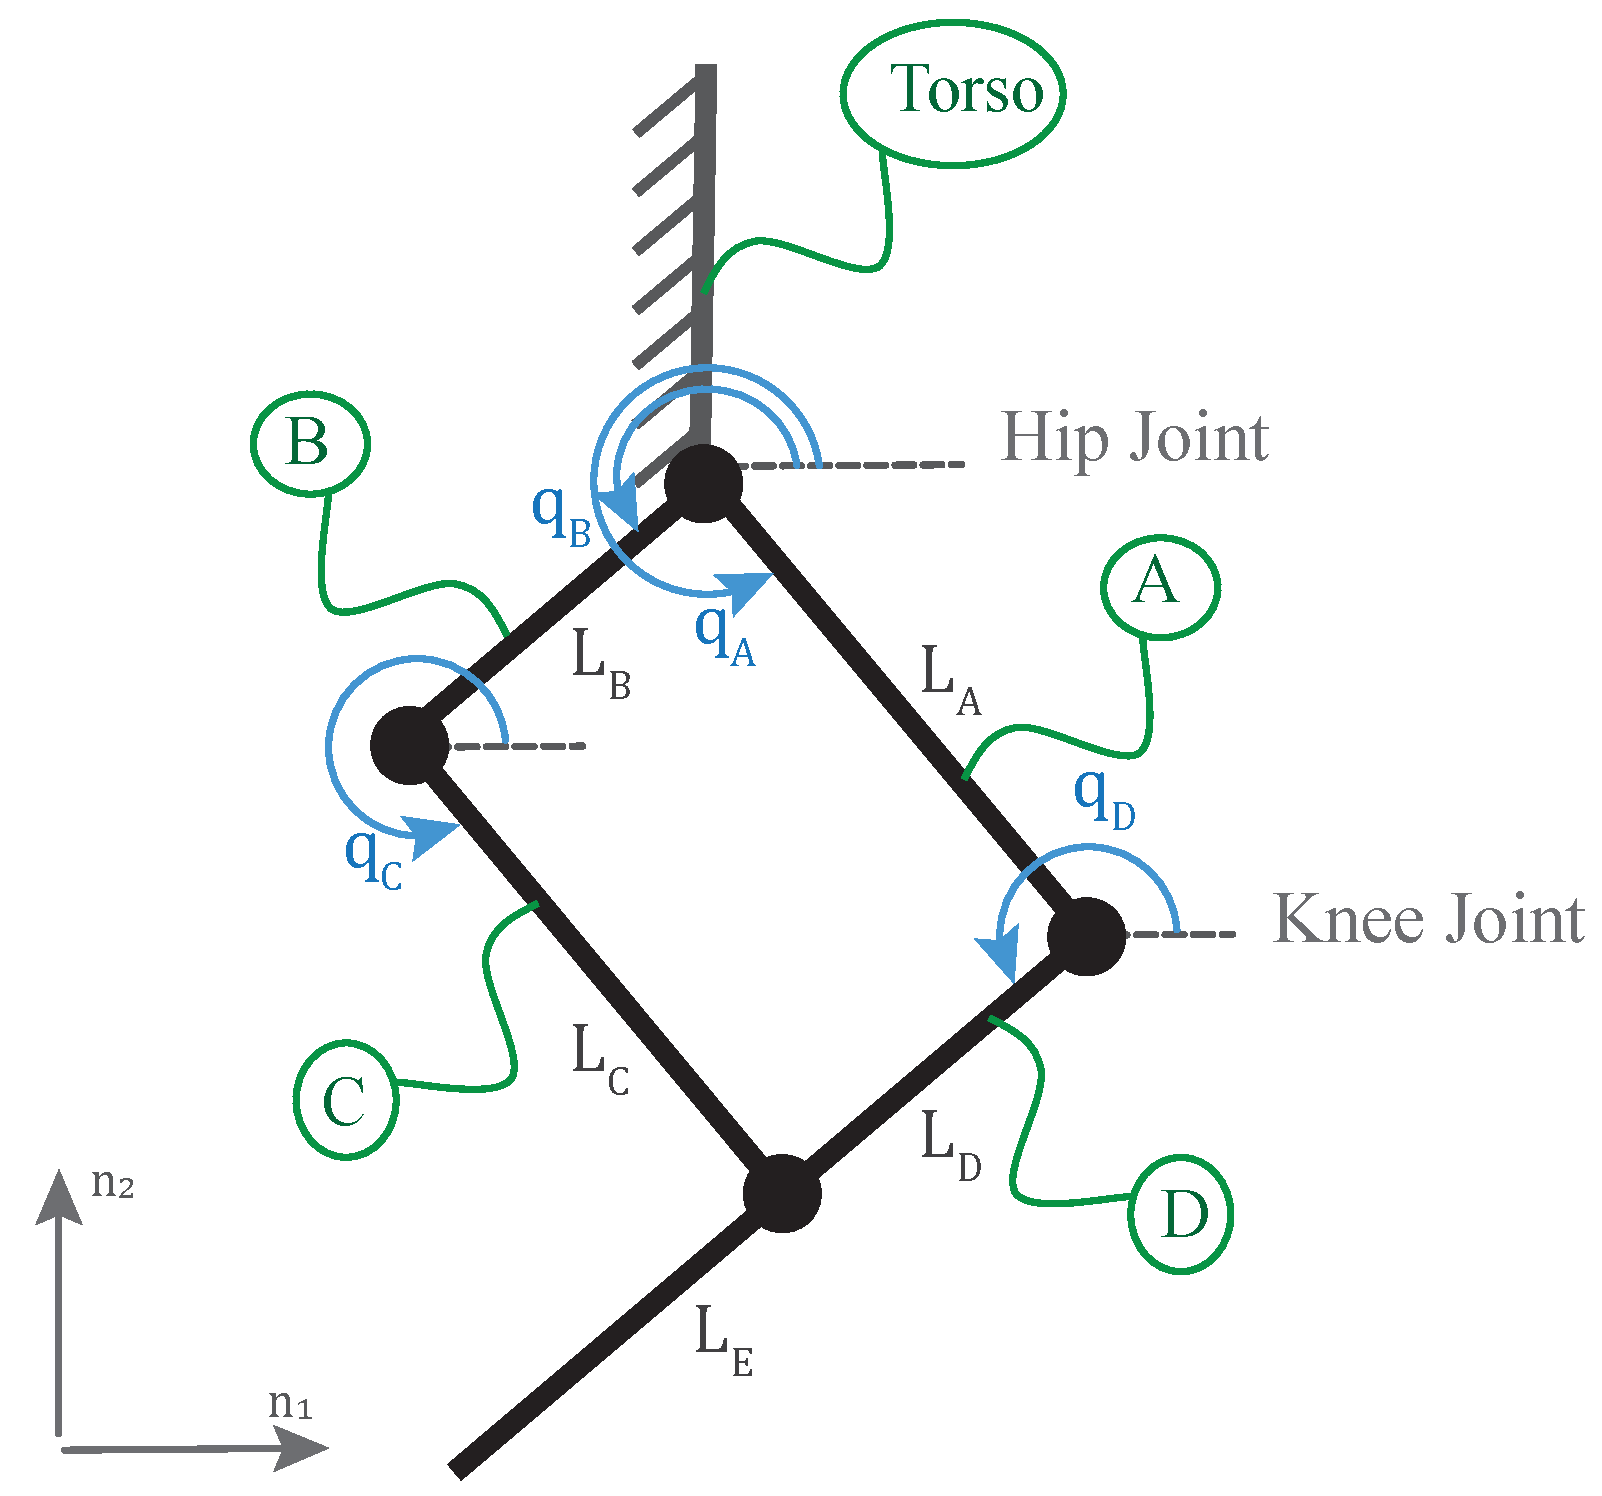
\includegraphics[width=2in]{Cartoons/Biarticular_Exo_Mechanism.pdf}
		\label{Fig_Biarticular_Exo_Mechanism}}
	\hfil
	\subfloat[\small{monoarticular device}]{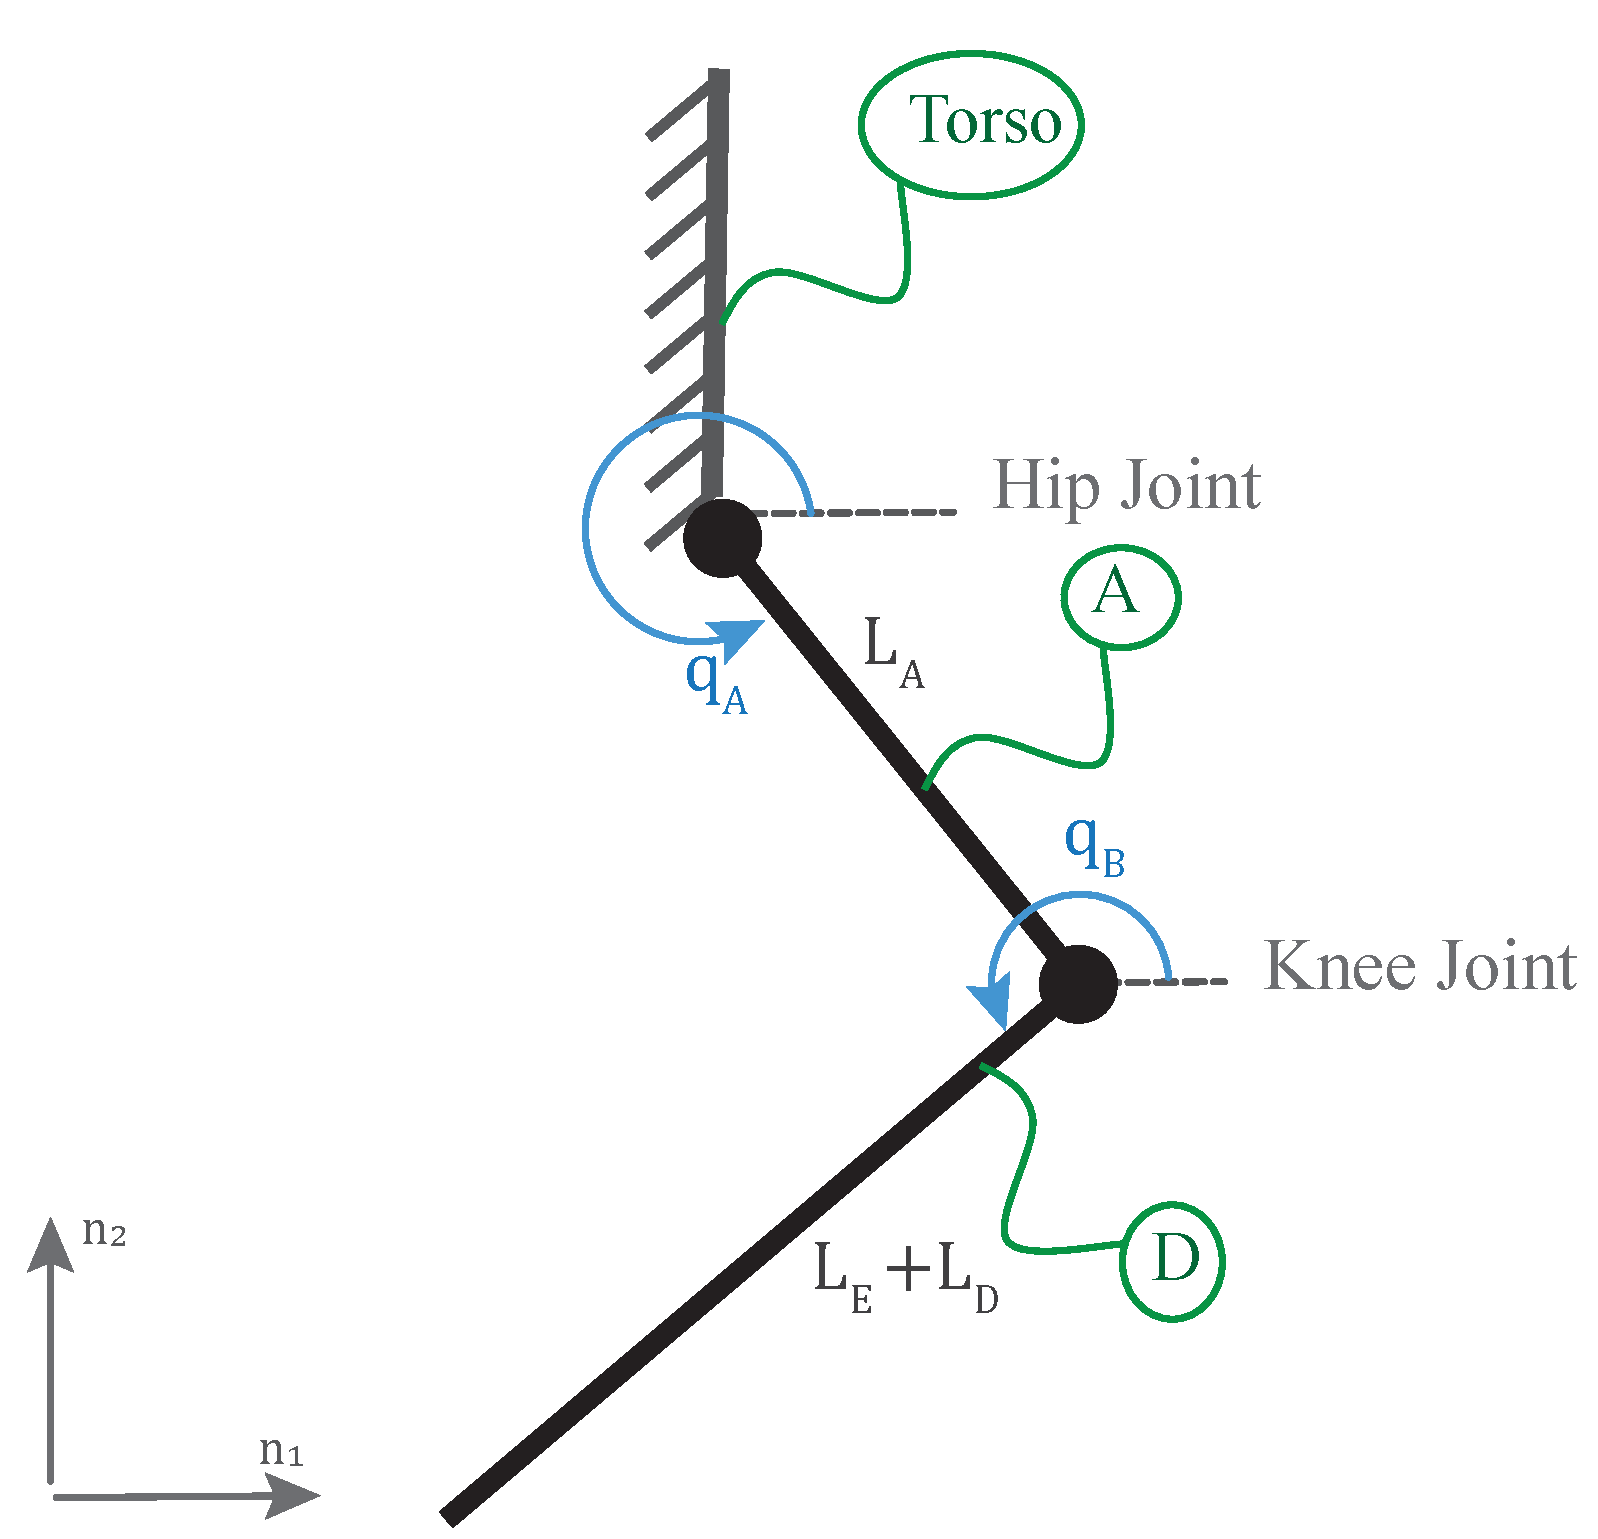
\includegraphics[width=2in]{Cartoons/Monoarticular_Exo_Mechanism.pdf}
		\label{Fig_Monoarticular_Exo_Mechanism}}
	\vspace{1mm}
	\caption{\small{\textbf{Assistive devices kinematics model.} The parallelogram mechanism has been used to model the biarticular exoskeleton and the monoarticular exoskeleton modeled by two link serial manipulator.}}
	\label{Fig_Exos_Kinematics_Model}
\end{figure*}
Where the hip joint will be assisted by applying directly the torque on the joint and second actuator torque will be applied to knee joint through the parallelogram mechanism where kinematics is 
\begin{align}\label{Eqn_Bi_Kin}
x_{Bi} &= l_ {A}\cos (q_ {A}) + (l_ {E} + l_ {D})\cos (q_ {B})\\
y_{Bi} &= l_ {A}\sin (q_ {A}) + (l_ {E} + l_ {D})\sin (q_ {B})
\end{align}

Monoarticular Exoskeleton can be modeled as a two-link serial manipulator as shown in figure \ref{Fig_Exos_Kinematics_Model}\subref{Fig_Monoarticular_Exo_Mechanism} where each joint is assisted by the directly joint actuator and the forward kinematics of monoarticular exoskeleton is:

\begin{align}\label{Eqn_Mono_Kin}
x_{mono} &= l_ {A}\cos (q_ {A}) + (l_ {E} + l_ {D})\cos (q_ {A} - q_ {B})\\
y_{mono} &= l_ {A}\sin (q_ {A}) + (l_ {E} + l_ {D})\sin (q_ {A} - q_ {B})
\end{align}
For both of the exoskeletons configurations the kinematics in motion level also can be easily driven and resulted Jacobian of each configurations can be written as in Eq \eqref{Eqn_Bi_Jacobian} and \eqref{Eqn_Mono_Jacobian}.

\begin{gather}\label{Eqn_Bi_Jacobian}
J_{Bi} =
\begin{bmatrix}
-l_{A}\sin{q_{A}}  & -(l_ {E} + l_ {D})\sin (q_ {B})\\
l_ {A}\cos (q_{A}) &  (l_ {E} + l_ {D})\cos (q_ {B})
\end{bmatrix}_{2 \times 2}
\end{gather}

\begin{equation}\label{Eqn_Mono_Jacobian}
\begin{aligned}
J_{Mono}&=
\left[\begin{matrix}
-l_{A}\sin{q_{A}}- (l_ {E} + l_ {D})\sin (q_ {A} - q_ {B})\\
l_{A}\cos{q_{A}} + (l_{E} + l_{D})\cos (q_{A} - q_ {B})
\end{matrix}\right.\\
&\qquad\qquad
\left.\begin{matrix}
{} (l_ {E} + l_ {D})\sin (q_ {A} - q_ {B})\\
{} - (l_ {E} + l_ {D})\cos (q_ {A} - q_ {B})
\end{matrix}\right]_{2\times 2}
\end{aligned}
\end{equation}
As it can be interpreted from the kinematics of exoskeletons, there is a jacobian between monoarticular and biarticular exoskeletons as it is represented in Eqn \ref{Eqn_Mono_Bi_Jacobian}.
\begin{equation}\label{Eqn_Mono_Bi_Jacobian}
\begin{aligned}
\omega_{2\times 1, \mathrm{monoarticular}} &= J_{2\times 2}\omega_{2\times 1, \mathrm{biarticular}}\\
\left\lbrack \begin{array}{c}
{}^{\mathrm{torso}} {\omega_{\mathrm{mono}} }^{\mathrm{femur}} \\
{}^{\mathrm{femur}} {\omega_{\mathrm{mono}} }^{\mathrm{tibia}} 
\end{array}\right\rbrack &=\left\lbrack \begin{array}{cc}
1 & 0\\
-1 & 1
\end{array}\right\rbrack \left\lbrack \begin{array}{c}
{}^{\mathrm{torso}} {\omega_{\mathrm{bi}} }^{\mathrm{femur}} \\
{}^{\mathrm{torso}} {\omega_{\mathrm{bi}} }^{\mathrm{tibia}} 
\end{array}\right\rbrack
\end{aligned}
\end{equation}
Using Eqn \ref{Eqn_Mono_Bi_Jacobian} which is a mapping between the angular velocities of the exoskeletons, we can derive the mapping between the provided torque by exoskeletons.
\begin{equation*}
\begin{aligned}
\tau{}_{2\times 1,\;\mathrm{biarticular}}^T \omega {}_{2\times 1,\mathrm{biarticular}} &=\tau {}_{2\times 1,\;\mathrm{monoarticular}}^T \omega {}_{2\times 1,\mathrm{monoarticular}}\\
\tau {\;}_{2\times 1,\;\mathrm{biarticular}}^T \omega {\;}_{2\times 1,\mathrm{biarticular}} &=\tau {\;}_{2\times 1,\;\mathrm{monoarticular}}^T J\omega {\;}_{2\times 1,\mathrm{monoarticular}}\\
\end{aligned}
\end{equation*}
Rewriting the equations more clearly, we can express the torque mapping explicitly as Eqn.\ref{Mono_Bi_Torque_Mapping}.
\begin{equation}\label{Mono_Bi_Torque_Mapping}
\begin{aligned}
\tau_{2\times 1,\;\mathrm{biarticular}} &=J^T \tau_{2\times 1,\;\mathrm{monoarticular}}\\
\left\lbrack \begin{array}{c}
{\tau^{\mathrm{torso}/\mathrm{femur}} }_{\mathrm{bi}} \\
{\tau^{\mathrm{torso}/\mathrm{tibia}} }_{\mathrm{bi}} 
\end{array}\right\rbrack &={\left\lbrack \begin{array}{cc}
	1 & 0\\
	-1 & 1
	\end{array}\right\rbrack }^T \left\lbrack \begin{array}{c}
{\tau^{\mathrm{torso}/\mathrm{femur}} }_{\mathrm{mono}} \\
{\tau^{\mathrm{femur}/\mathrm{tibia}} }_{\mathrm{mono}} 
\end{array}\right\rbrack\\
\end{aligned}
\end{equation}
This relation between two exoskeleton has been used to verify the modeling of the exoskeleton through musculoskeletal simulation framework.
%%%%%%%%%%%%%%%%%%%%%%%%%%%%%%%%%%%%%%%%%%%%%%%%%%%%%%%%%%%%%%%%%%%%%%%%%%%%%%%%%%%%%%%%%
%%%%%%%%%%%%%%%%%%%%%%%%%%%%%%%%%%%%%%%%%%%%%%%%%%%%%%%%%%%%%%%%%%%%%%%%%%%%%%%%%%%%%%%%%
\section*{\textbf{Musculoskeletal Simulation}}
%%%%%%%%%%%%%%%%%%%%%%%%%%%%%%%%%%%%%%%%%%%%%%%%%%%%%%%%%%%%%%%%%%%%%%%%%%%%%%%%%%%%%%%%%
\subsection*{Musculoskeletal Model}
The exoskeletons have been studied through musculoskeletal simulations by conducting the simulations of the seven subjects walking normally and while carrying a 38kg load on the torso at their chosen speed. The data that has been used in this study was experimentally collected and processed by Dembia et.al. \cite{93} and their experimental protocol was approved by the Stanford University Institutional Review Board \cite{93}.\\
The musculoskeletal model used in the simulations, which was the same with the model used by dembia et al. \cite{93}, was a three-dimensional model developed by Rajagopal et al. \cite{130} with 39 degrees of freedom where the lower limbs were actuated using 80 massless musculotendon actuators, and the upper limb actuated by 17 torque actuators\cite{130}. \\
This three-dimensional musculoskeletal model was adapted by locking some unnecessary degrees of freedom for both normal walking and walking with a heavy load scenarios and modeling the extra load on the torso of the musculoskeletal model for the walking with heavy load condition \cite{93}.\\
Since this research was built upon the study performed by Dembia et al., we will follow the similar terminologies in most of the cases to avoid any confusion for the readers. Therefore, the \textit{loaded} condition will refer to the subjects walking while carrying the 38Kg load on their torso while the \textit{noload} condition will reference the subjects walking without any extra load at their self chosen speed.
%%%%%%%%%%%%%%%%%%%%%%%%%%%%%%%%%%%%%%%%%%%%%%%%%%%%%%%%%%%%%%%%%%%%%%%%%%%%%%%%%%%%%%%%%
\subsection*{Simulation Procedure}
The first step for conducting the simulation of the specific subject is scaling the generic dynamic model to acquire a musculoskeletal model matching with the anthropometry of the subject which was performed using OpenSim Scale Tool and according to the mass and height of the subject, the maximum isometric forces of the muscles were scaled. After obtaining the specific model for the subject, inverse kinematics of the subject were computed using OpenSim Inverse Kinematics Tool and the motion capture data collected experimentally.\\
On the next stage of the simulation workflow, the scaled model, inverse kinematics and ground reaction forces were employed to run the RRA algorithm\cite{103}. The RRA algorithm reduces the incompatibility of experimental data including ground reaction forces and trace data and musculoskeletal model by slightly adjusting inertial properties and kinematics. Then adjusted model and kinematics generated by RRA were employed to perform muscle driven simulations using Computed muscle control algorithm in OpenSim\cite{104}.\\
Computed Muscle Control (CMC) algorithm simulates the muscle recruitment of the subject by resolving muscle redundancy problem using static optimization to find the required muscle excitations to track the provided kinematics. The CMC simulations output were then used to run the analysis tool of OpenSim to compute subjects metabolic power consumption, and muscles moment.\\
\begin{figure*}[ht]
	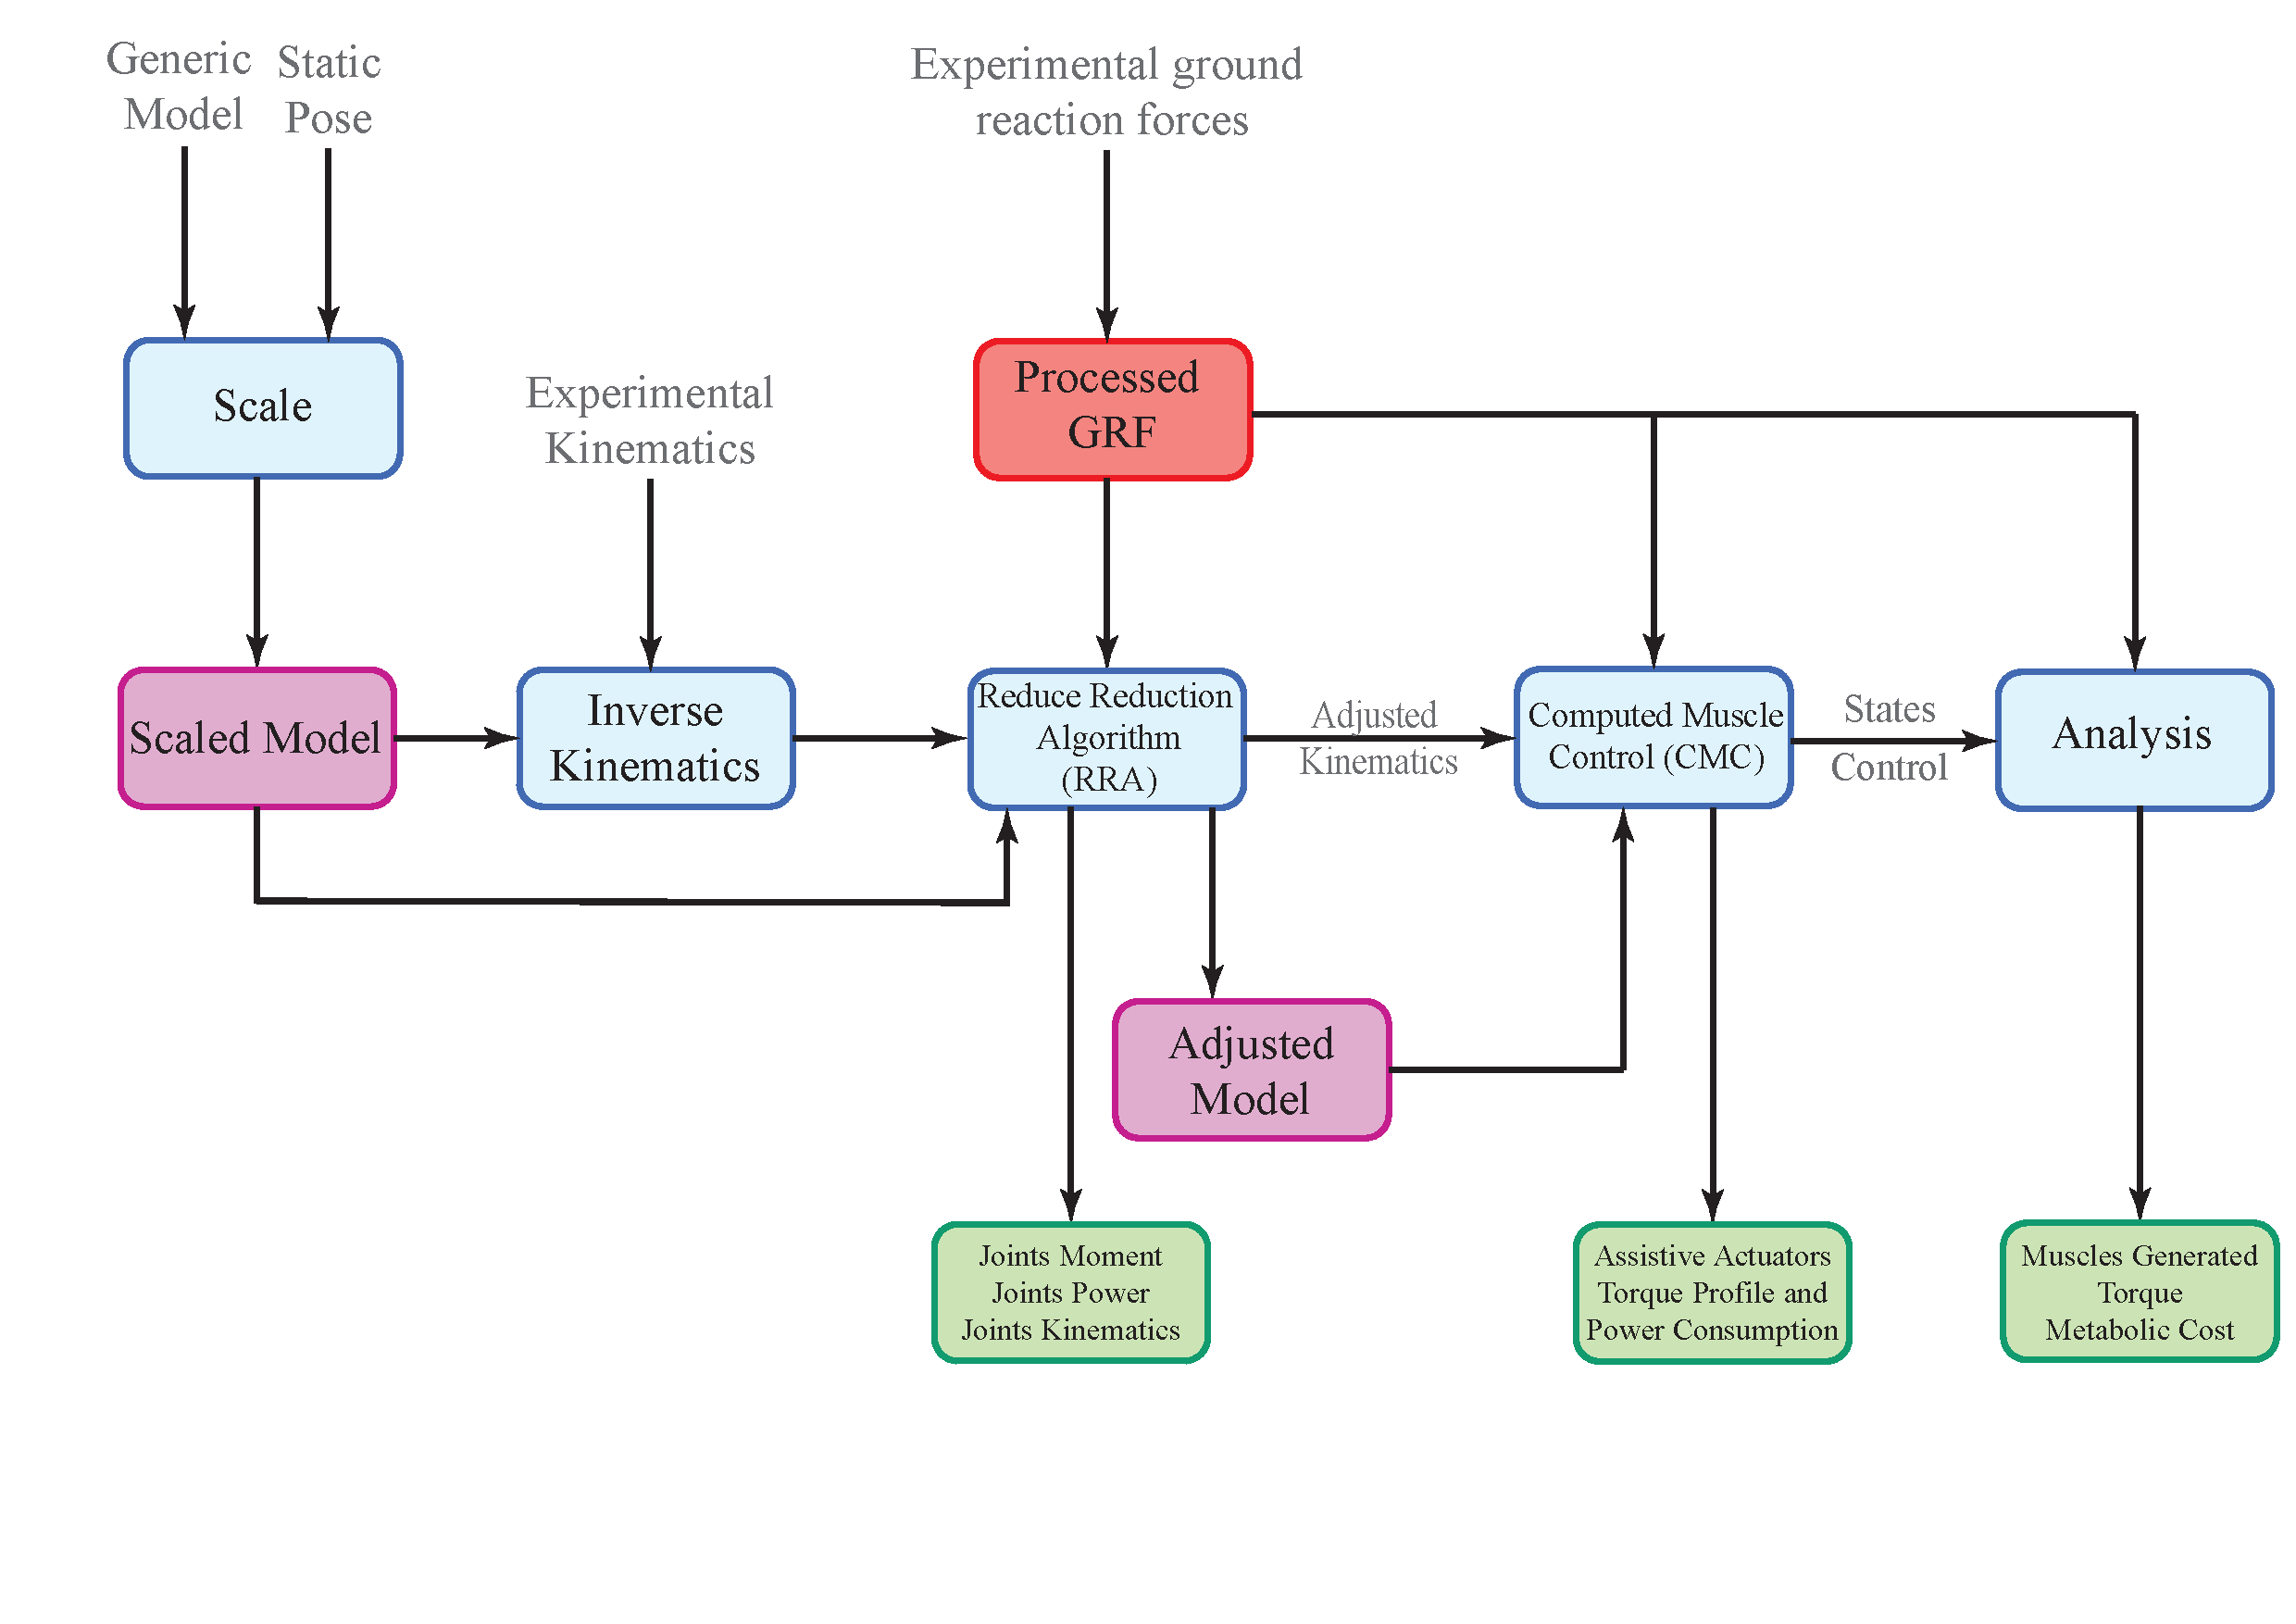
\includegraphics[width=\linewidth]{Cartoons/OpenSim.pdf} 
	\vspace{-5mm}
	\caption{\small{\textbf{Opensim simulation procedure block diagram.} The workflow of the simulation in OpenSim has been shown briefly in which green blocks stands for output, blue blocks are OpenSim simulations or analyses, purple blocks are models that have been used for simulations and analyses, and finally, red blocks represent processed experimental data.}}
	\label{Fig_OpenSim_Sim_Procedure}
\end{figure*}
The OpenSim solves the muscle redundancy problem to track experimentally measured motion and uses effort-based objective, as Eqn. \ref{Eqn_CMC_Objective}, to solve for a set of muscle excitations to track measured motions and forces within a specified tolerance using static optimization at each time step during the motion of interest\cite{92}. Therefore, the kinematics and dynamics of the subject will remain consistent during the simulations and any additional mass and inertia on the subject that has not been captured by experiments will cause a systematic error on the results.\\
\begin{equation}\label{Eqn_CMC_Objective}
J = \sum_{i\in nMuscles} a_{i}^{2} + \sum_{i \in nReserves} (\frac{\tau_{r,i}}{w_{r,i}})^2
\end{equation}
With the knowledge of the OpenSim neural control algorithm, we used the adjusted model and kinematics provided by Dembia et al.\cite{93} instead of reproducing all data from the beginning of the simulation procedure which also helped us to ease the verification of the simulations procedure thanks to \cite{93} for verified simulations data.\\
\textbf{Metabolic Model.} To calculate the estimation of the instantaneous metabolic power of subjects, Umberger \cite{105} muscle energetic model which was modified by Uchida et al. \cite{106}  were employed in which average power consumption of a muscle during a gait cycle was calculated using Eq.\ref{Eqn_avg_muscle_power} \cite{106}.\\
\begin{equation}\label{Eqn_avg_muscle_power}
	P_{avg} = \frac{m}{t_1 - t_0}\int_{t_0}^{t_1} \dot{E(t)} dt
\end{equation}
Where m is muscle mass, and $\dot{E(t)}$ is the normalized metabolic power consumed. This model generates metabolic power of all muscles and then whole body metabolic power was calculated by summing all muscles metabolic power \cite{106}. For computing the gross metabolic energy consumption of subjects, we integrated the metabolic power over the gait cycle and then divided by the mass of subjects.\\
As it is mentioned in \cite{93}, due to experimental data insufficiency, some subjects and trials simulation were not a complete gait cycle, therefore, the metabolic energy were calculated for a half of a gait cycle for these subjects and trials which is a verified method for computing the energy according to \cite{93}. \\
%%%%%%%%%%%%%%%%%%%%%1%%%%%%%%%%%%%%%%%%%%%%%%%%%%%%%%%%%%%%%%%%%%%%%%%%%%%%%%%%%%%%%%%%%
\subsection*{Modeling and simulation of assisted subjects}
The kinematics of the exoskeletons were already discussed and in order to model ideal exoskeletons in OpenSim framework we used the Torque Actuators provided by OpenSim API\cite{103}. Biarticular and Monoarticular exoskeletons' torque actuators were assigned, as shown in figure \ref{Fig_Exos_Model_Opensim}.
\begin{figure*}[h!]
	\centering
	\subfloat[\small{biarticular device}]{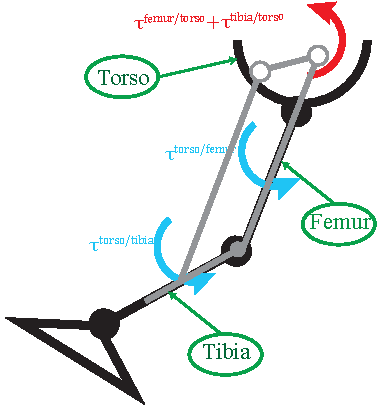
\includegraphics[width=2in]{Cartoons/Biarticular_Exo_Assignment.pdf}
		\label{Fig_Bi_Exo_Model_Opensim}}
	\hfil
	\subfloat[\small{monoarticular device}]{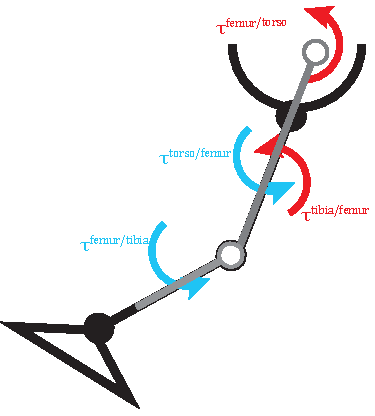
\includegraphics[width=2in]{Cartoons/Monoarticular_Exo_Assignment.pdf}
		\label{Fig_Mono_Exo_Model_Opensim}}
	\vspace{1mm}
	\caption{\small{\textbf{Assistive devices modeling on OpenSim.} The modeling of the hip and knee assistive devices in OpenSim framework in which TorqueActuators provided by opensim has been utilized to model the exoskeletons. The blue and red torques represent the action and reaction torques of the assistive actuators on the bodies.}}
	\label{Fig_Exos_Model_Opensim}
\end{figure*}
As it is represented in figure \ref{Fig_Exos_Model_Opensim} \subref{Fig_Bi_Exo_Model_Opensim}, both torque actuators of biarticular exoskeleton were assigned to torso , then, reaction forces of the actuators were applied to the torso which is in the match with the kinematics and dynamics model of the biarticular exoskeleton.
\begin{align}\label{Eqn_Biarticular_Torque_Act}
\tau^{hip}_{Biarticular} = \tau^{torso/femur}\\
\tau^{knee}_{Biarticular} = \tau^{torso/tibia}
\end{align}
Monoarticular exoskeleton (figure \ref{Fig_Exos_Model_Opensim} \subref{Fig_Mono_Exo_Model_Opensim}) modeled by assigning hip joint actuator from torso to femur body and knee joint actuator assigned from femur to tibia body where knee torque actuator's reaction torque applied to femur body:
\begin{align}\label{Eqn_Monoarticular_Torque_Act}
\tau^{hip}_{Monoarticular} = \tau^{torso/femur}\\
\tau^{knee}_{Monoarticular} = \tau^{femur/tibia}
\end{align}
\newline
\newline
\textbf{Computed Muscle Control adjusted objective function.} To investigate the performance of the assistive devices and their effect on human musculoskeletal system through OpenSim simulation framework we used the CMC algorithm. Computed Muscle Control algorithm objective function depends on the sum of squared muscle activation and reserve actuators, which compensates for modeled passive structures and potential muscle weakness\cite{93}:
\begin{equation}\label{Eqn_CMC_Normal_Obj_Func}
J = \sum_{i\in nMuscles} a_{i}^{2} + \sum_{i \in nReserves} (\frac{\tau_{r,i}}{w_{r,i}})^2
\end{equation}
Where $w_i$ determines the weight of reserve actuators which is generally selected as a small number to highly penalize using of reserve actuators. By adding assistive device actuators (i.e. Torque Actuators) to the musculoskeletal model of the subject they will be added to the CMC tool objective function. The adjusted objective function will include the assistive actuators as it is expressed in Eq. \eqref{Eqn_CMC_Assisted_Obj_Func} and by selecting proper weights for the assistive actuators, they can be chosen by the optimizer as the actuation of the assigned degree of freedom.
\begin{equation}\label{Eqn_CMC_Assisted_Obj_Func}
	J = \sum_{i\in nMuscles} a_{i}^{2} + \sum_{i \in nExo} \left(\frac{\tau_{exo,i}}{w_{exo,i}}\right)^{2} +  \sum_{i \in nReserves} \left(\frac{\tau_{r,i}}{w_{r,i}}\right)^2
\end{equation}
In the adjusted objective function, $w_{exo,i}$ is torque actuator weights which is named optimal force in OpenSim \cite{93} penalizing the usage of torque actuators. By selecting a large number, penalization of the actuators will be insignificant and they will be selected for actuating the joint between two bodies assigned for torque actuator and if we select a small optimal force, the optimizer will highly penalize the usage of exoskeleton actuators.To study each configuration of the exoskeleton in their maximum performance, the assigned torque actuator's optimal force was selected as 1000 N.m enabling the optimizer to use the assistive actuators as much as possible during a gait cycle simulation.\\
\vspace{5mm}
\textbf{Metabolics and actuators energy calculation.} Similar to the unassisted procedure, the instantaneous metabolic power of the subjects was computed using the energetic model of Uchida et al. \cite{106} and then metabolic energy of subjects were derived by integration of the metabolic power over the gait cycle. In order to compute the energy consumption of the assistive actuators, the power profile of the actuators were obtained and their absolute power profiles were integrated over the gait cycle and divided to the subjects mass. Similar to the energy consumption of the exoskeleton procedure, the negative energy or regeneratable energy through a gait cycle were calculated by obtaining the negative power profile and integrated over the gait cycle and normalized to the mass of the subject.\\
%%%%%%%%%%%%%%%%%%%%%%%%%%%%%%%%%%%%%%%%%%%%%%%%%%%%%%%%%%%%%%%%%%%%%%%%%%%%%%%%%%%%%%%%%
\subsection*{Pareto Simulations}
The optimization stage of the Computed Muscle Control (CMC) algorithm uses the weighted sum of squares to solve muscles and assigned actuators redundancy to select a set of actuation with the lowest cost for tracking the kinematics of the dynamic model of the subject \cite{92}. To investigate the ideal assistive devices maximum effect on the subjects metabolic power consumption regardless of their energy expenditure, large weights were assigned to assistive actuator.\\
However, in the real-time, exoskeletons are restricted by the energy that can be supplied to the actuation module and the maximum torque that the actuation module can provide to the joint of interest; to study devices performance under the maximum providable torque to the joints and their effect on musculoskeletal system in lower energy consumption regions, we used the Pareto-Optimization concept\cite{113}.\\
Pareto method integrates all optimization criteria in its procedure and constructs a Pareto front representing trade-off among the criteria enabling us to have optima curves for each configuration of the devices \cite{107} and conduct a fair comparison between the exoskeletons and the load conditions. In this study, metabolic cost reduction and assistive actuators energy consumption were considered as two optimization criteria to study the trade-off between the exoskeletons and load conditions.\\
One of the acceptable Pareto front is a discrete set of Pareto-optima points obtained by constructing a single objective function by integrating objectives and optimizing the single cost function throughout the specific range of values of the parameters used to combine the cost functions into a single objective function \cite{108}.\\
The pareto optimization method has been used by M. L. Handford and M. Srinivasan\cite{111,127} to study robotic lower limb prostheses by simultaneously optimizing the metabolic and prosthesis cost rate. \\

\textbf{The workflow of the Pareto-simulations.} To accomplish the simulations of the Pareto-optimization in the OpenSim framework, we constrained the peak torque of assistive actuators constraining the objective function mentioned in Eq \ref{Eqn_CMC_Assisted_Obj_Func} throughout a specific range from high to low providable torque throughout a gait cycle changing the solution of the optimizer for muscles and actuator redundancy problem. This variation over the discrete range of maximum providable torque resulting in different points on the optimization objectives space and by filtering points, we achieved to Pareto front for each configuration of the exoskeleton.\\
For the biarticular and monoarticular exoskeletons in both \textit{loaded} and \textit{noload} conditions, the maximum torque of the actuators were varied between 30 N.m and 70 N.m. For performing the simulations, the constraint of the hip actuator was fixed and the constraint of the knee was varied; after simulating all of the exoskeletons with a fixed hip constraint and varying knee constraint, the constraint of the hip actuator was changed for performing the next iteration of the simulations. The algorithm has been shown the following pseudo code.\\

\begin{algorithm}\label{Algorithm_Pareto_simulation}
	\caption{Pareto Simulations Algorithm}\label{Pareto_Algorithm}
	\begin{algorithmic}[1]
		\For{$i = [70,60,50,40,30]$}
		\For{$j = [70,60,50,40,30]$}
		\State Set $\{-i,i\}$ : hip actuators constraint: $\{Min Control, Max Control\}$
		\State Set $\{-j,j\}$ : knee actuators constraint: $\{Min Control, Max Control\}$
		\State Update exoskeleton model by the new constraints
		\State Perform \textbf{CMC} Simulation
		\EndFor
		\EndFor
	\end{algorithmic}
\end{algorithm}
\textbf{Inertial properties of the exoskeletons effect on metabolic rate.} One of the main challenges with designing the mobile exoskeletons is the effect of the mass and inertia, grounded on the extremities of the subjects, on the metabolic rate of the subjects. The effect of mass and inertia on the metabolic cost has been studied through several literatures \cite{133,134} and shown that metabolic rate of the subject would change considerably by adding mass and inertia \cite{133,134,135}.\\
The proposed exoskeleton in this studies have a remarkable difference from the inertial properties due to their kinematic design and it will result in different effect on the metabolic rate of the subjects.\\
Since the current neural control algorithm of the OpenSim is not able to simulate any variations in the musculoskeletal model, which has not been captured by experimental data, we simulated the effect of the mass and inertia offline using the metabolic model of the Browning et al.\cite{133}. This study proposed a linear model for the effect of adding mass and inertia on each segment of lower limbs by capturing and analyzing these effects experimentally. In the study accomplished by Browning et al.\cite{133}, subjects were walking at 1.25 m/s without carrying any heavy load on their torso which is similar to the data captured from the subjects in the walking with \textit{\textit{noload}} at their self-selected speed\cite{93}. This qualitative match between the data and experimental protocols of Browning et al. and Dembia et al enabling us to use the developed model of \cite{133}  to study the effect of mass and inertia added by assistive devices through offline simulations.\\
The mass and inertia of the proposed biarticular and monoarticular exoskeletons affect the waist, thigh and shank segments.As it is discussed in the Kinematic Modeling section, the biarticular exoskeleton, unlike monoarticular one, is designed to deliver the assistance distally to the knee joint.
It enables designers to attach actuation module to the waist instead of thigh meaning that the main difference between inertial properties of two exoskeletons will be on the attached mass on the waist and shank segments nevertheless the reflected inertia of the actuation module will be reflect on the actuated joint regardless of its grounded segment in both exoskeletons.\\
For the purpose of conducting numerical simulations of the inertial properties of the exoskeletons effect on the subjects metabolic rate, we assigned two identical masses and the center of masses measured from the hip and knee joints for the links attached to the thigh and shank respectively. Additionally,a typical and identical actuation module inertia and mass has been assigned for both configurations of the exoskeleton.\\
In order to study the effect of the inertia in the pareto simulations, the maximum achievable torque of the actuator has been set to 2 N.m which can be provided by MaxonMotor EC90 Flat 260W and the required transmission ratio is calculated by diving the peak torque at joint level to peak torque of the actuator and then reflected inertia has been calculated using Eqn.\ref{Eqn_reflected_inertia}.\\
\begin{equation}\label{Eqn_reflected_inertia}
	\begin{aligned}
	R &= \frac{\tau_{max,jont level}}{\tau_{max,actuator}}\\
	I_{reflected} &= I_{actuator}\times R^{2}
	\end{aligned}
\end{equation}
The inertia of the moving segments (i.e., thigh and shank segments) have been computed by considering the distal mass effect on the inertia, which is different for each configuration of the exoskeletons, reflected inertia of the actuation module and the leg inertia provided by \cite{133} which is calculated about center of rotation of the leg in the body frame. The Eqn.\ref{Eqn_segment_inertia} represents the inertia calculation of a segment.
\begin{equation}\label{Eqn_segment_inertia}
\begin{aligned}
I_{Exo,segment} &= I_{reflected} + m\times COM^{2}\\
I_{\textit{loaded}\;leg} &= I_{Exo,segment} + I_{\textit{\textit{noload}}\;leg}
\end{aligned}
\end{equation}
The typical mass, center of mass and inertia that have been used for numerical simulations are represented in Table \ref{Table_Exokeletons_Mass_Inerta}. These values are mostly in match with the mechanical properties of the biarticular and monoarticular exoskeletons designed in our lab.\\
\begin{table}[ht]
	\renewcommand{\arraystretch}{1.2}
	\begin{adjustwidth}{-1in}{0in}
		\caption{\small{\textbf{Mass and inertia properties of two typical exoskeletons.}}}
	\begin{tabular}{c!{\vline width 0.2pt}c!{\vline width 0.2pt}c!{\vline width 0.2pt}c!{\vline width 0.2pt}c!{\vline width 0.2pt}c!{\vline width 0.2pt}c}
		\toprule
		 \multirow{2}{*}{\textbf{configuration}} & \textbf{Waist}   & \multicolumn{2}{ c!{\vline width 0.2pt} }{\textbf{thigh}} & \multicolumn{2}{ c!{\vline width 0.2pt} }{\textbf{shank}} & \textbf{actuator} \\  \cmidrule{2-7}
		  &  Mass ($kg$)& mass ($kg$) & COM ($m$)& mass ($kg$) & COM ($m$)& inertia ($kg.m^2$) \\ \midrule[0.5pt]
		  \textbf{Biarticular} &  6 &1& 0.23 &0.9&0.18&$5.06\times10^{-4}$\\ \midrule[0.2pt]
		  \textbf{Monoarticular} & 4.5 &2.5& 0.30 &0.9&0.18&$5.06\times10^{-4}$\\
		  \bottomrule
	\end{tabular}
	\label{Table_Exokeletons_Mass_Inerta}
	\end{adjustwidth}
\end{table}
The metabolic model proposed by Browning et al.\cite{133} is calculating the metabolic rate of the subject with \textit{loaded} segment, however, Since we were interested in the effect of inertial properties of exoskeleton on metabolic rate change, not metabolic rate, we used the model by subtracting the metabolic rate of the subject walking without the additional mass. The equations of the final model that has been used for analyzing the effect of exoskeleton mass and inertia on the metabolic rate is provided in Eqn.\ref{Eqn_AddingMass_MetabolicRate} and \ref{Eqn_AddingInertia_MetabolicRate} respectively.
\begin{equation}\label{Eqn_AddingMass_MetabolicRate}
\begin{aligned}
\Delta MC_{Waist} &= 0.045\times m_{Waist}\\
\Delta MC_{Thigh} &= 0.075\times m_{Thigh}\\
\Delta MC_{Shank} &= 0.076\times m_{Shank}
\end{aligned}
\end{equation}
\begin{equation}\label{Eqn_AddingInertia_MetabolicRate}
\begin{aligned}
I_{ratio} &= \frac{I_{Exo,segment} + I_{un\textit{loaded}\;leg}}{I_{un\textit{loaded}\;leg}}\\
\Delta MC_{Thigh} &= ((-0.74 + (1.81\times I_{Thigh,ratio}))\times MC_{unassisted})-MC_{unassisted}\\
\Delta MC_{Shank} &= ((0.63749 + (0.40916\times I_{Shank,ratio}))\times MC_{unassisted})-MC_{unassisted}
\end{aligned}
\end{equation}
The effect of the exoskeleton mass and inertia has on metabolic cost has been considered on the pareto curves and filtered to obtain the pareto front with the effect of the exoskeleton inertial properties on metabolic expenditure.
%TODO: how they are added to the paretocurves and how they are filtered.
%%%%%%%%%%%%%%%%%%%%%%%%%%%%%%%%%%%%%%%%%%%%%%%%%%%%%%%%%%%%%%%%%%%%%%%%%%%%%%%%%%%%%%%%%
\subsection*{Validation of Simulations}
The comprehensive validation procedure of the OpenSim simulations was published by the Hicks et al. \cite{92} where they explained how to validate modeling and simulation results at each stage. Additionally, Dembia et al. \cite{93} explained simulation verification for their assistive device simulations and we followed the same procedures explained in \cite{92,93} to validate our results from the simulations.\\
As it is already discussed, the adjusted model, adjusted kinematics and processed ground reaction forces that has been provided by \cite{93} have been used for accomplishing this study which has been evaluated and validated by Dembia et al. \cite{93}. As it is recommended in \cite{92}, the muscular activation resulted from the simulation has been validated with the experimentally recorded electromyography (EMG) signals.\\
The \textit{loaded} and \textit{\textit{noload}} joint kinematics and kinetics were compared with the results of the studies accomplished by Huang and Kuo \cite{131} and Silder et al.\cite{132} and validated qualitatively. Since our simulations of the unassisted subject for \textit{loaded} and \textit{noload} conditions were the same with Dembia et al. simulations, we reproduced their simulations and compared them with their results to validate our reproduced simulations results. Additionally, since we used the provided RRA results for performing the CMC simulations, the joint moment and joint kinematics represented in this paper were already validated.\\
The other source of error during the simulations are kinematics and residual errors which were analyzed to be in the recommended thresholds\cite{92}; nevertheless, since the inverse kinematics stage of simulation was not reproduced in this study, the markers error was not examined. Another error source in these simulations could be additional moments introduced to compensate any modeled passive structures and muscles weakness where it is recommended to have less than 5\% of net joint moments in peak and RMS \cite{92}. It has been checked for all simulations and confirmed that the reserve actuator torques are smaller than the recommended percentage of joint moments.
%%%%%%%%%%%%%%%%%%%%%%%%%%%%%%%%%%%%%%%%%%%%%%%%%%%%%%%%%%%%%%%%%%%%%%%%%%%%%%%%%%%%%%%%%
\subsection*{Performance Metrics}
%TODO: We may add two new performance metrics but their data need to be extracted and plotted.
For the purpose of having methodical analysis and comparison between the assistive devices and load conditions some performance metrics have been defined. As discussed earlier, the ultimate goal of each assistive device is reducing energy consumed by the subject for performing a task which is walking with and without load at normal speed in this study.
Therefore, we calculated the normalized gross whole-body metabolic rate of the subjects in two different assistive devices and load conditions and then metabolic cost reduction has been computed using the metabolic rate of assisted and unassisted subjects. This procedure of metabolic cost calculation was repeated for all seven subjects in three trials to obtain the total average metabolic energy expenditure and metabolic cost reduction for each assistance scenario and load condition.\\
Another important metrics for assessing the performance of an exoskeleton is the energy it consumes to provide the assistance. To analyze this metrics in the simulated exoskeletons, we computed the absolute energy consumed by the all actuators and the reason for considering the absolute value is absence of the regeneration mechanism as a general case for the exoskeletons. On the other hand, in order to analyze the amount of energy available for regeneration, we computed the negative energy of the exoskeletons. This metric is a crucial part of the untethered exoskeletons analysis to estimate the battery life.\\
At the pareto optimization part of the study, these two metrics (i.e., metabolic cost reduction and energy consumption) are represented together by averaging them for each defined constraints over the subjects and represented with mean and standard deviation for both criteria. This metric represents the set of different configurations for each exoskeleton in terms of energy consumption and the amount of assist the device can provide. For more detailed analyses, some specific congifurations in each exoskeleton and load condition have been selected and compared in more comprehensive manner.\\
Additionally, the effect of regeneratable energy and inertial properties of the exoskeletons, as two important metrics for analyzing the performance of the assistive devices, have been studied in pareto simulations by reflecting their effect on the Pareto-curves and obtaining the pareto sets affected by these two metrics.
Finally, some of the muscular activations of the lower limb key muscles were extracted and studied to have insight into how an assistive device can change muscles activities and consequently, metabolic cost which is resulted from muscles activities.
\subsection*{Statistical Analysis}
To conduct methodical comparisons among scenarios with the discussed metrics, we employed statistical analyses. Since the simulations were performed on seven subjects with three trials in five different scenarios, repeated measures analysis of variance (ANOVA) and Tukey Post-hoc were applied to test the statistically significant difference between the selected metrics and scenarios.  Additionally, for the pareto simulations, the statistical analysis has been performed for the specific points selected from the pareto front for further investigation, nevertheless, standard deviation of all points on pareto front has been explicitly plotted for both criteria. We used a significance level of 0.05 and SPSS \cite{spss} for performing the tests. Same as \cite{93}, to remove the hierarchical structure from the data, they were averaged over the trials for each subject-scenario pair. However, the time-dependent data are averaged over all subjects and their trials and represented by their mean and standard deviation.
%%%%%%%%%%%%%%%%%%%%%%%%%%%%%%%%%%%%%%%%%%%%%%%%%%%%%%%%%%%%%%%%%%%%%%%%%%%%%%%%%%%%%%%%%
%%%%%%%%%%%%%%%%%%%%%%%%%%%%%%%%%%%%%%%%%%%%%%%%%%%%%%%%%%%%%%%%%%%%%%%%%%%%%%%%%%%%%%%%%
\section*{\textbf{Results and Discussion}}
%TODO: The results are changed by averaging within trials for each subject and getting overal average for all averaged subjects
%%%%%%%%%%%%%%%%%%%%%%%%%%%%%%%%%%%%%%%%%%%%%%%%%%%%%%%%%%%%%%%%%%%%%%%%%%%%%%%%%%%%%%%%%
\subsection*{Ideal Exoskeletons Results}
%%%%%%%%%%%%%%%%%%%%%%%%%%%%%%%%%%%%%%%%%%%%%%%%%%%%%%%%%%%%%%%%%%%%%%%%%%%%%%%%%%%%%%%%%
\subsubsection*{Device Performance}
Both biarticular and monoarticular configurations of the ideal exoskeletons reduced the metabolic energy consumption of subjects walking without and with carrying a heavy load at self-selected speed walking. Biarticular and monoarticular exoskeletons decreased the subjects carrying a heavy load metabolic rate by 20.49$\pm$2.87\% and 20.45$\pm$2.81\%. The monoarticular and biarticular configurations of the exoskeleton were able to reduce the gross whole-body metabolic cost of the subject in the \textit{noload} condition by 22.38$\pm$4.91\% and 22.47$\pm$4.89\%. These exoskeletons were expected to have the same performance on reducing the metabolic energy consumption of the subjects due to their kinematic relation, and the results are representing the expected performance for these two devices.\\
\begin{figure*}[ht]   
	\centering
	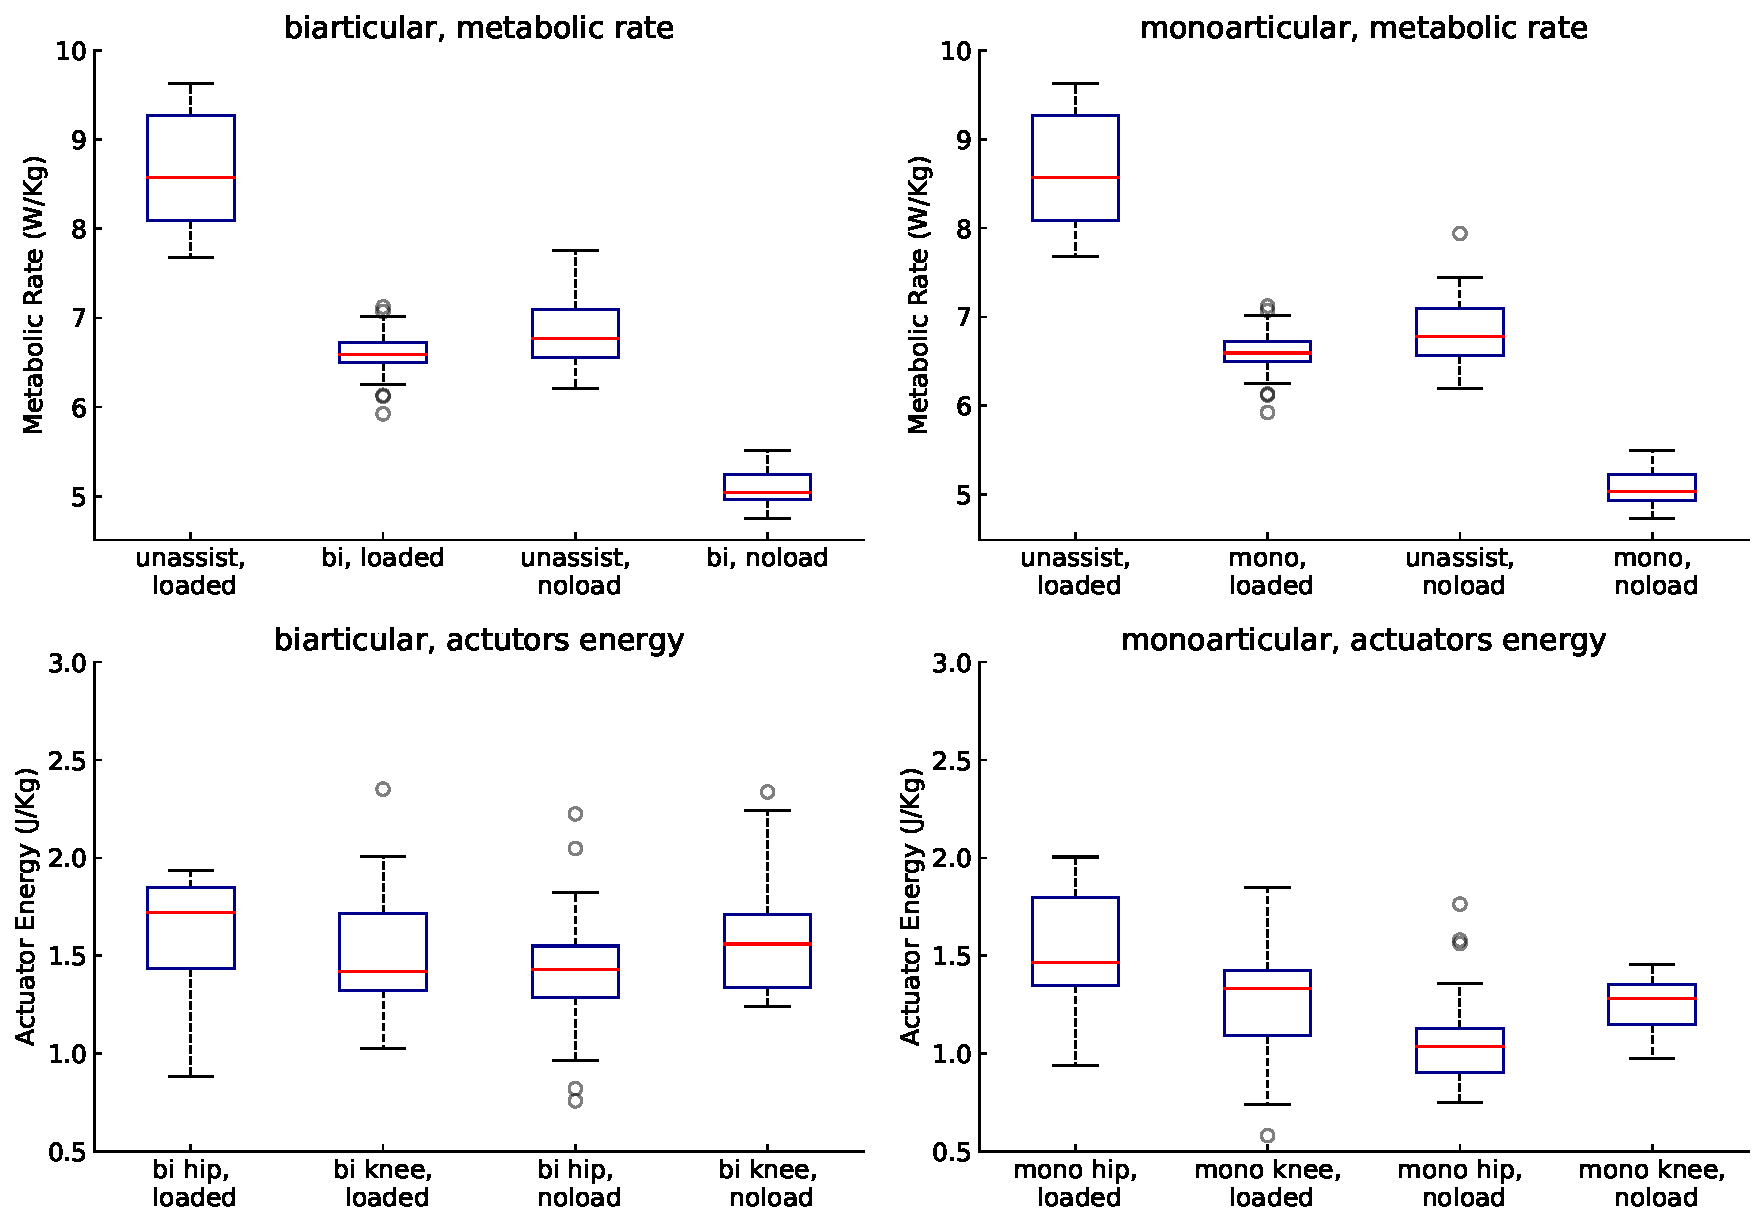
\includegraphics[width=\linewidth]{Ideal_Exo_MonovsBi_Figures/Paper_Figure_Energy_BoxPlot.pdf}
	\vspace{1mm}
	\caption{\small{\textbf{Assistive devices and metabolic power.} The power consumptions of assistive devices and their effect on whole-body metabolic rate of the subjects walking with and without carrying a heavy load.}}
	\label{Fig_IdealExo_Energy_BoxPlot}
\end{figure*}
The assistance of both exoskeletons on subjects carrying a heavy load was able to compensate for demanding metabolic energy for carrying the heavy load. As it can be seen in figure \ref{Fig_IdealExo_Energy_BoxPlot}, the assisted subjects in \textit{loaded} condition have a similar metabolic rate with unassisted subjects do not carry any load meaning that the best both ideal exoskeletons can do is reducing the metabolic energy-demanding of the \textit{loaded} subject to subject without any load.\\
The energy consumption of both exoskeletons has a high within-subject variation on the \textit{loaded} condition comparing to the \textit{noload} condition. While monoarticular exoskeleton had less energy consumption in both knee and hip actuators and both conditions, but these differences are not statistically significant between the two exoskeletons.  Although both exoskeletons have considerably different hip actuator energy consumption between \textit{noload} and \textit{loaded} conditions, the significant difference between the loading conditions of the subjects cannot be observed for energy expenditure of the knee actuator in both configurations.\\
%%%%%%%%%%%%%%%%%%%%%%%%%%%%%%%%%%%%%%%%%%%%%%%%%%%%%%%%%%%%%%%%%%%%%%%%%%%%%%%%%%%%%%%%%
\subsubsection*{Devices Speed, Torque and Power}
One of the main objectives of this section is to validate the kinematic modeling of the exoskeleton on OpenSim. As it is already discussed, there is a mapping between monoarticular and biarticular exoskeletons, and if the modeling of the devices were correct in the musculoskeletal simulator, this kinematics relation requires to be held.\\
The figure \ref{Fig_IdealExo_Speed} represents the velocity profiles of the biarticular and monoarticular exoskeletons in both load conditions. From the Eqn. \ref{Eqn_Mono_Bi_Jacobian} we were expecting to have the same angular velocity profiles hip actuator, and since hip actuator in both exoskeletons were supposed to be attached directly to the hip joint, the velocity of the joint and actuators in both devices have practically the same profiles as it is shown in figure \ref{Fig_IdealExo_Speed}  for hip joints in both load conditions.\\
\begin{figure*}[ht]   
	\centering
	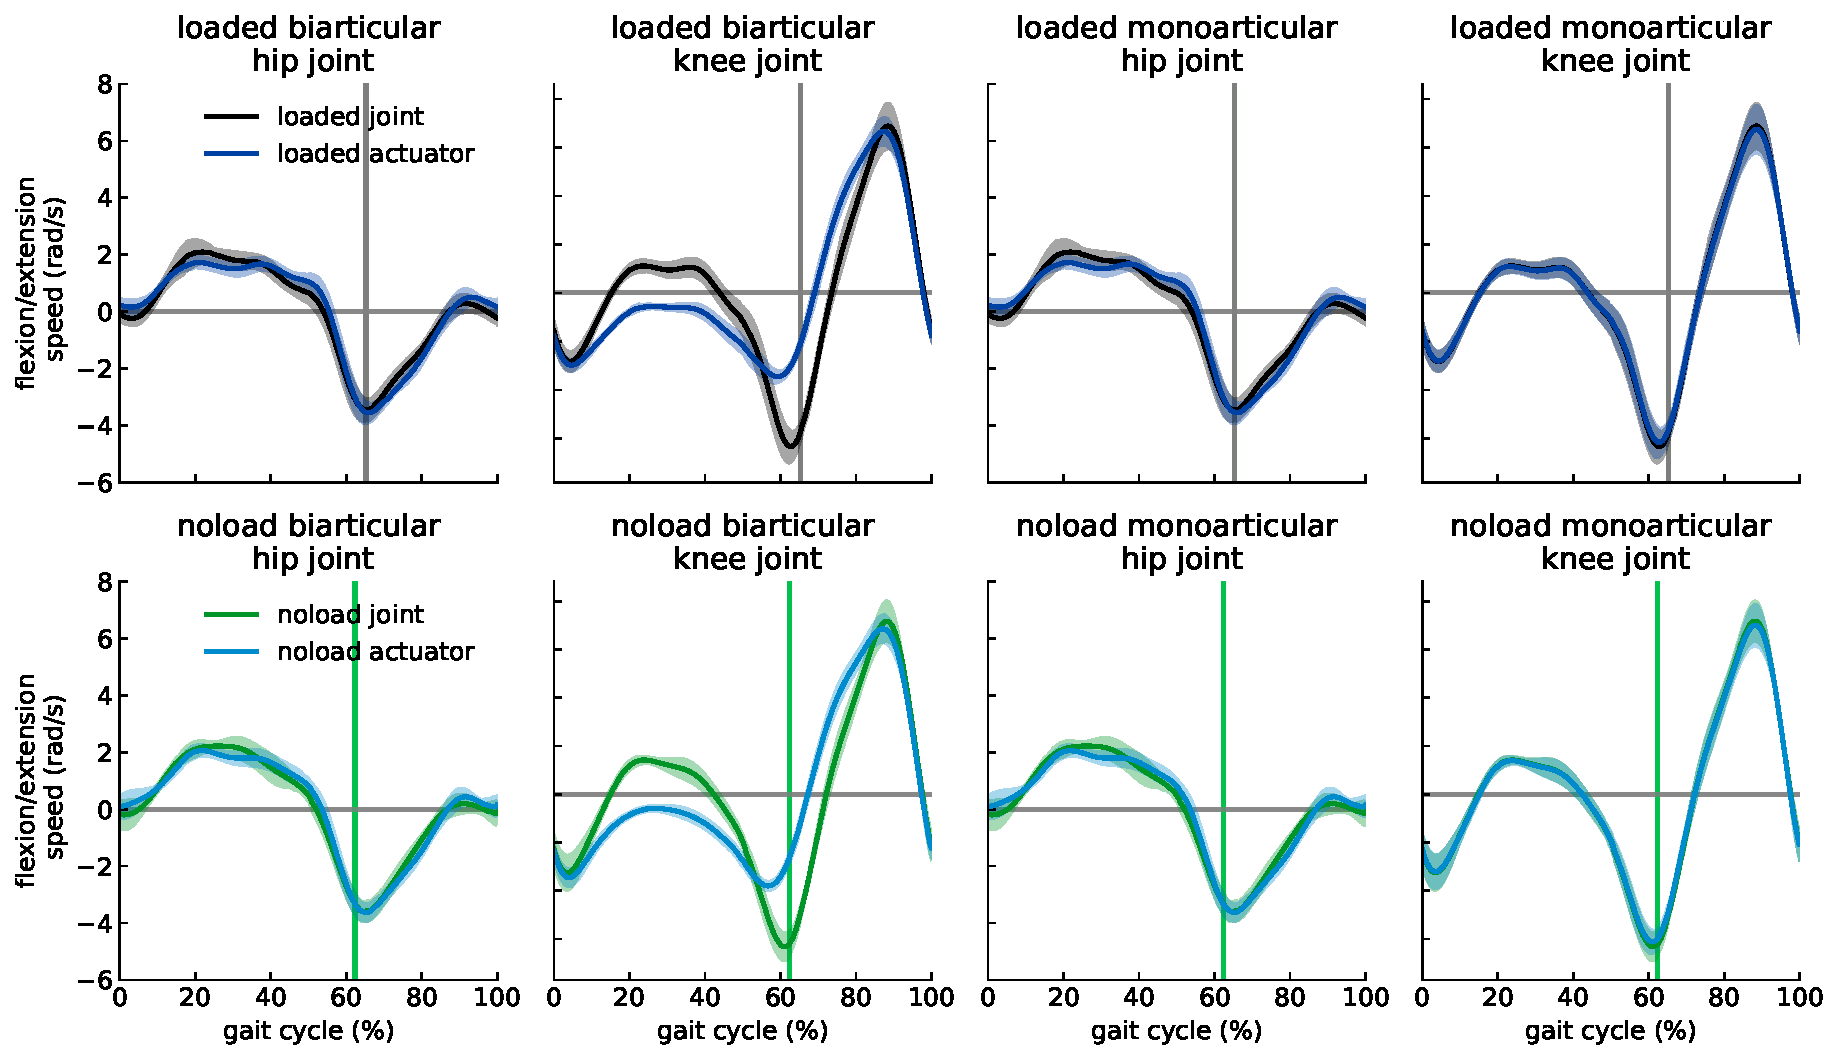
\includegraphics[width=\linewidth]{Ideal_Exo_MonovsBi_Figures/PaperFigure_Exoskeletons_Speed.pdf}
	\vspace{1mm}
	\caption{{\small\textbf{Assistive devices velocity profiles compared to joint required velocities.} The device actuator velocity for subjects carrying heavy load (dark blue) and without any load (blue), and net joint velocity profile for \textit{loaded} (black) and \textit{noload} (green) conditions are shown for each actuator of the devices. The curves are averaged over 7 subjects with 3 trials; shaded regions around the mean profile indicate standard deviation of the profile.}}
	\label{Fig_IdealExo_Speed}
\end{figure*}
The main difference between the two configurations of the exoskeleton is on the knee joint, where the biarticular device assists the joint through a parallelogram mechanism, and the velocity profiles of the knee actuator were supposed to be different according to their jacobian. This difference can be seen in the figure \ref{Fig_IdealExo_Speed} where monoarticular knee actuator follows the knee joint velocity profile, but the biarticular actuator is showing different profile than the knee joint profile due to Eqn. \ref{Eqn_Mono_Bi_Jacobian}. Analyzing velocity profiles of the devices validating the mapping between two exoskeletons and modeling of them through OpenSim.\\
According to the jacobian between these two devices expressed in Eqn. \ref{Mono_Bi_Torque_Mapping}, the knee and hip actuators were expected to have the same and different torque profiles respectively, which is evident in figure \ref{Fig_IdealExo_Torque} for both \textit{loaded} and \textit{noload} conditions. The generated optimal torque profiles of the ideal exoskeletons did not resemble the net moment of the assisted joint, which was also observed by \cite{93,2} for the simulation-based study of the walking with heavy load and running respectively. The torque of assistive actuators in both hip and knee joints exceeded the corresponding net joint moment and resulted in opposing muscles generated moment and device torque in the joint.\\
\begin{figure*}[ht]   
	\centering
	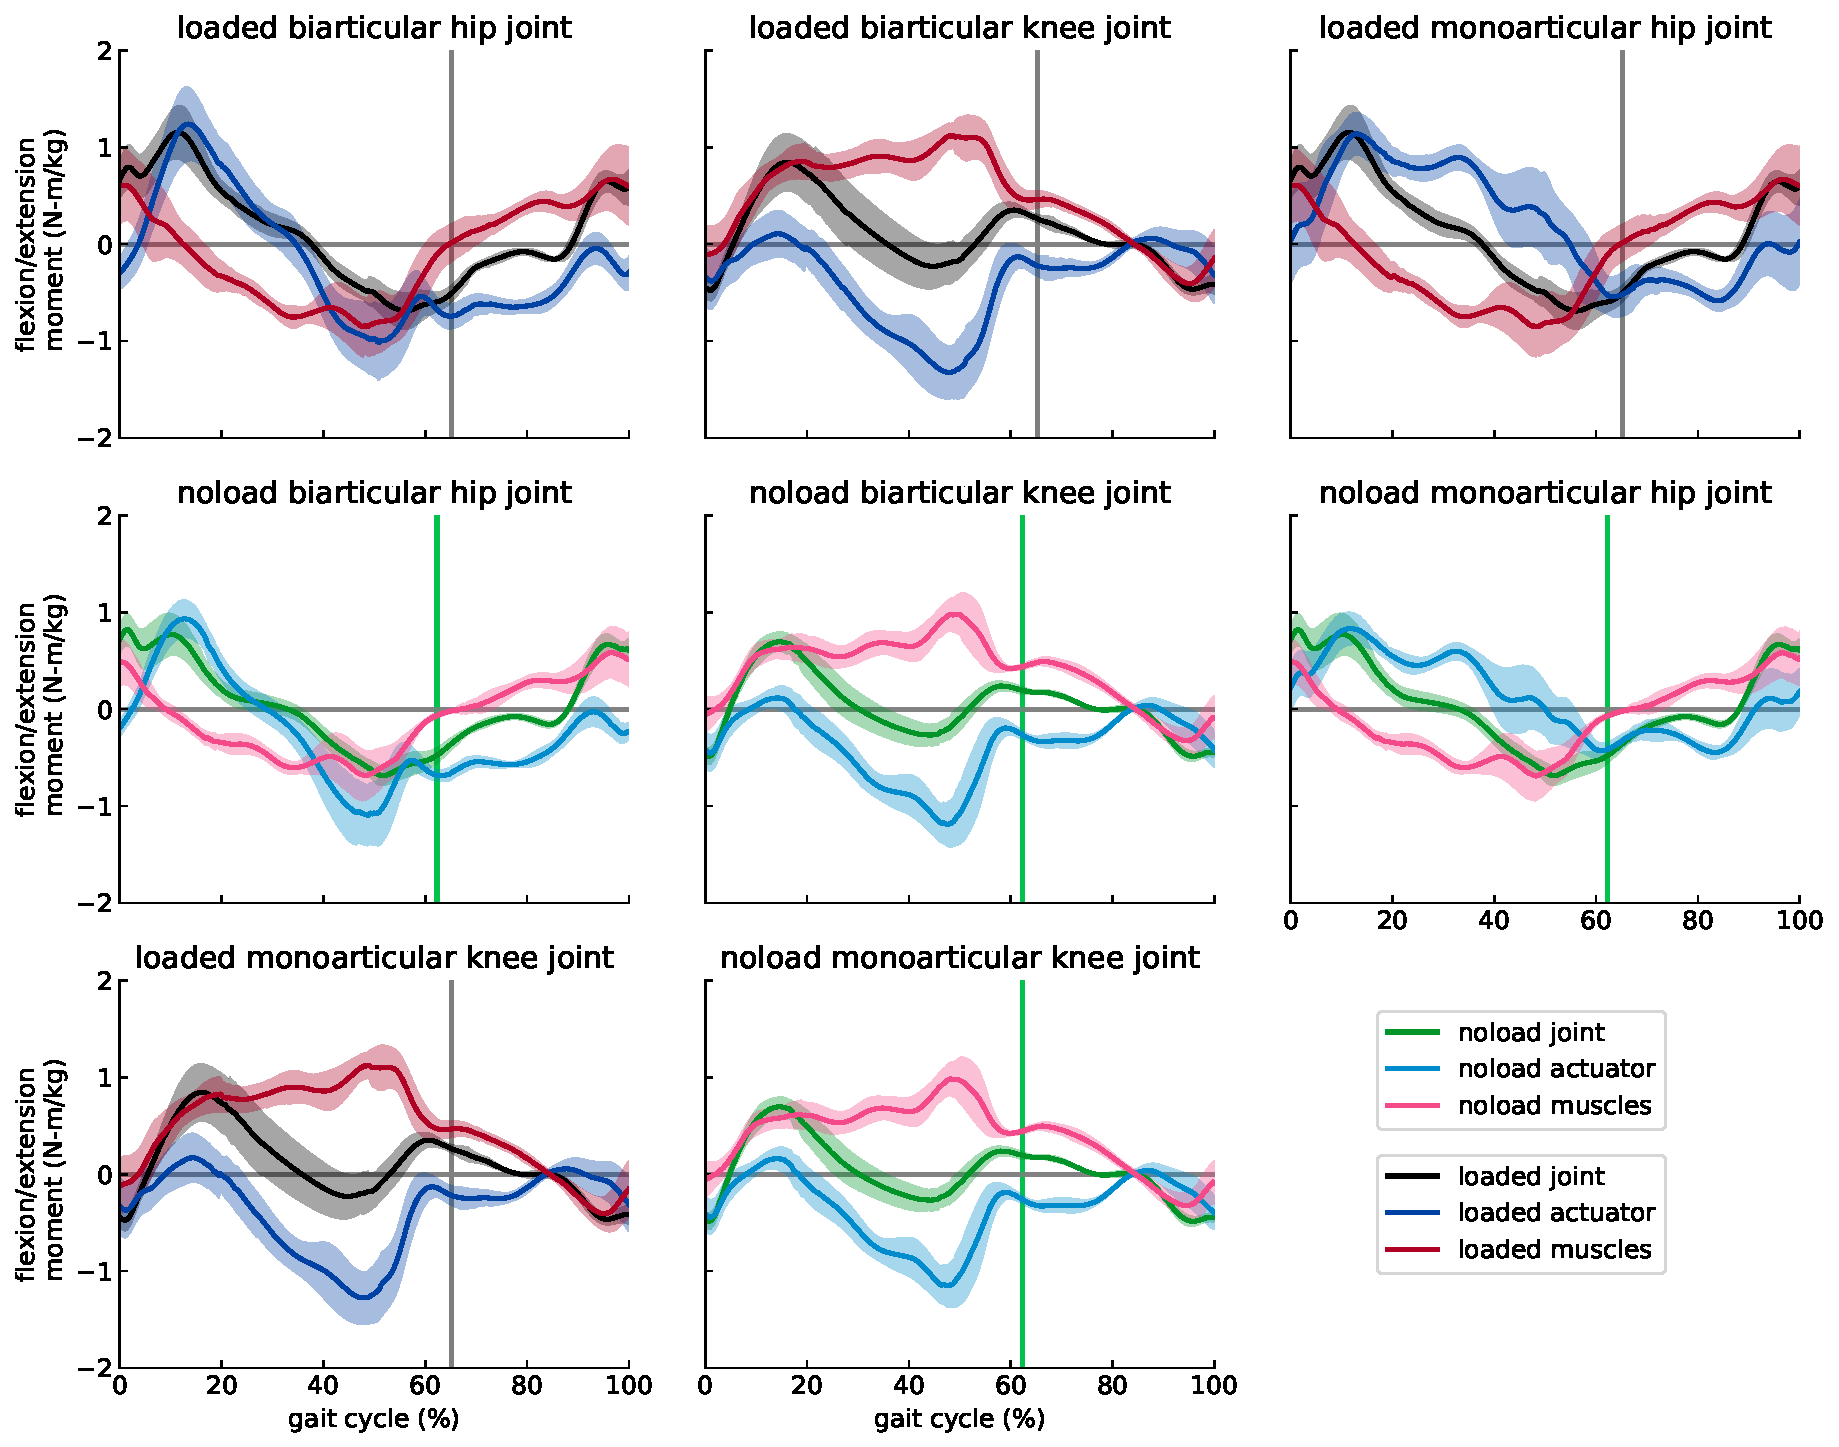
\includegraphics[width=\linewidth]{Ideal_Exo_MonovsBi_Figures/PaperFigure_Exoskeletons_Torque.pdf}
	\vspace{1mm}
	\caption{{\small\textbf{Assistive devices torque profiles compared to joint and muscles generated moment.} The device actuator torque for subjects carrying heavy load (dark blue) and without any load (blue), net joint moment profile generated by unassisted muscles for \textit{loaded} (black) and \textit{noload} (green) conditions, and the generated moment by assisted muscles for \textit{loaded} (dark rose red) and \textit{noload} (rose red) conditions are shown for each actuator of the devices. The curves are averaged over 7 subjects with 3 trials and normalized by subject mass; shaded regions around the mean profile indicate standard deviation of the profile.}}
	\label{Fig_IdealExo_Torque}
\end{figure*}
This antagonism is more significant on the knee joint than hip during the mid-stance phase to the mid-swing phase, with the highest opposition on the start of the pre-swing phase. The hip joint has significant actuator and muscle torque opposition during the pre-swing to terminal swing phases meaning unlike the knee joint in which major portion of antagonism happens during the stance phase; the hip is getting into muscle and actuator torque contraction during swing phase. \\
The torque profiles represented in figure \ref{Fig_IdealExo_Torque} indicate that the loading subject with a heavy load does not result in substantial changes in the torque profiles of the assistive devices. The main changes between \textit{loaded} and \textit{noload} conditions are the timing and magnitude of the profiles, which is due to the change of the joints kinematics and kinetics.
Nevertheless, the standard deviation of assistive devices and assisted muscles generated torques are considerably greater in the \textit{loaded} condition, and it is more evident in the knee joint where the net joint moment has a remarkable deviation during the stance phase. This high within-subject deviation of torque profiles indicates that the assistance of subjects carrying heavy load requires the subject-specific design of the exoskeletons \cite{2}.\\
\begin{figure*}[ht]   
	\centering
	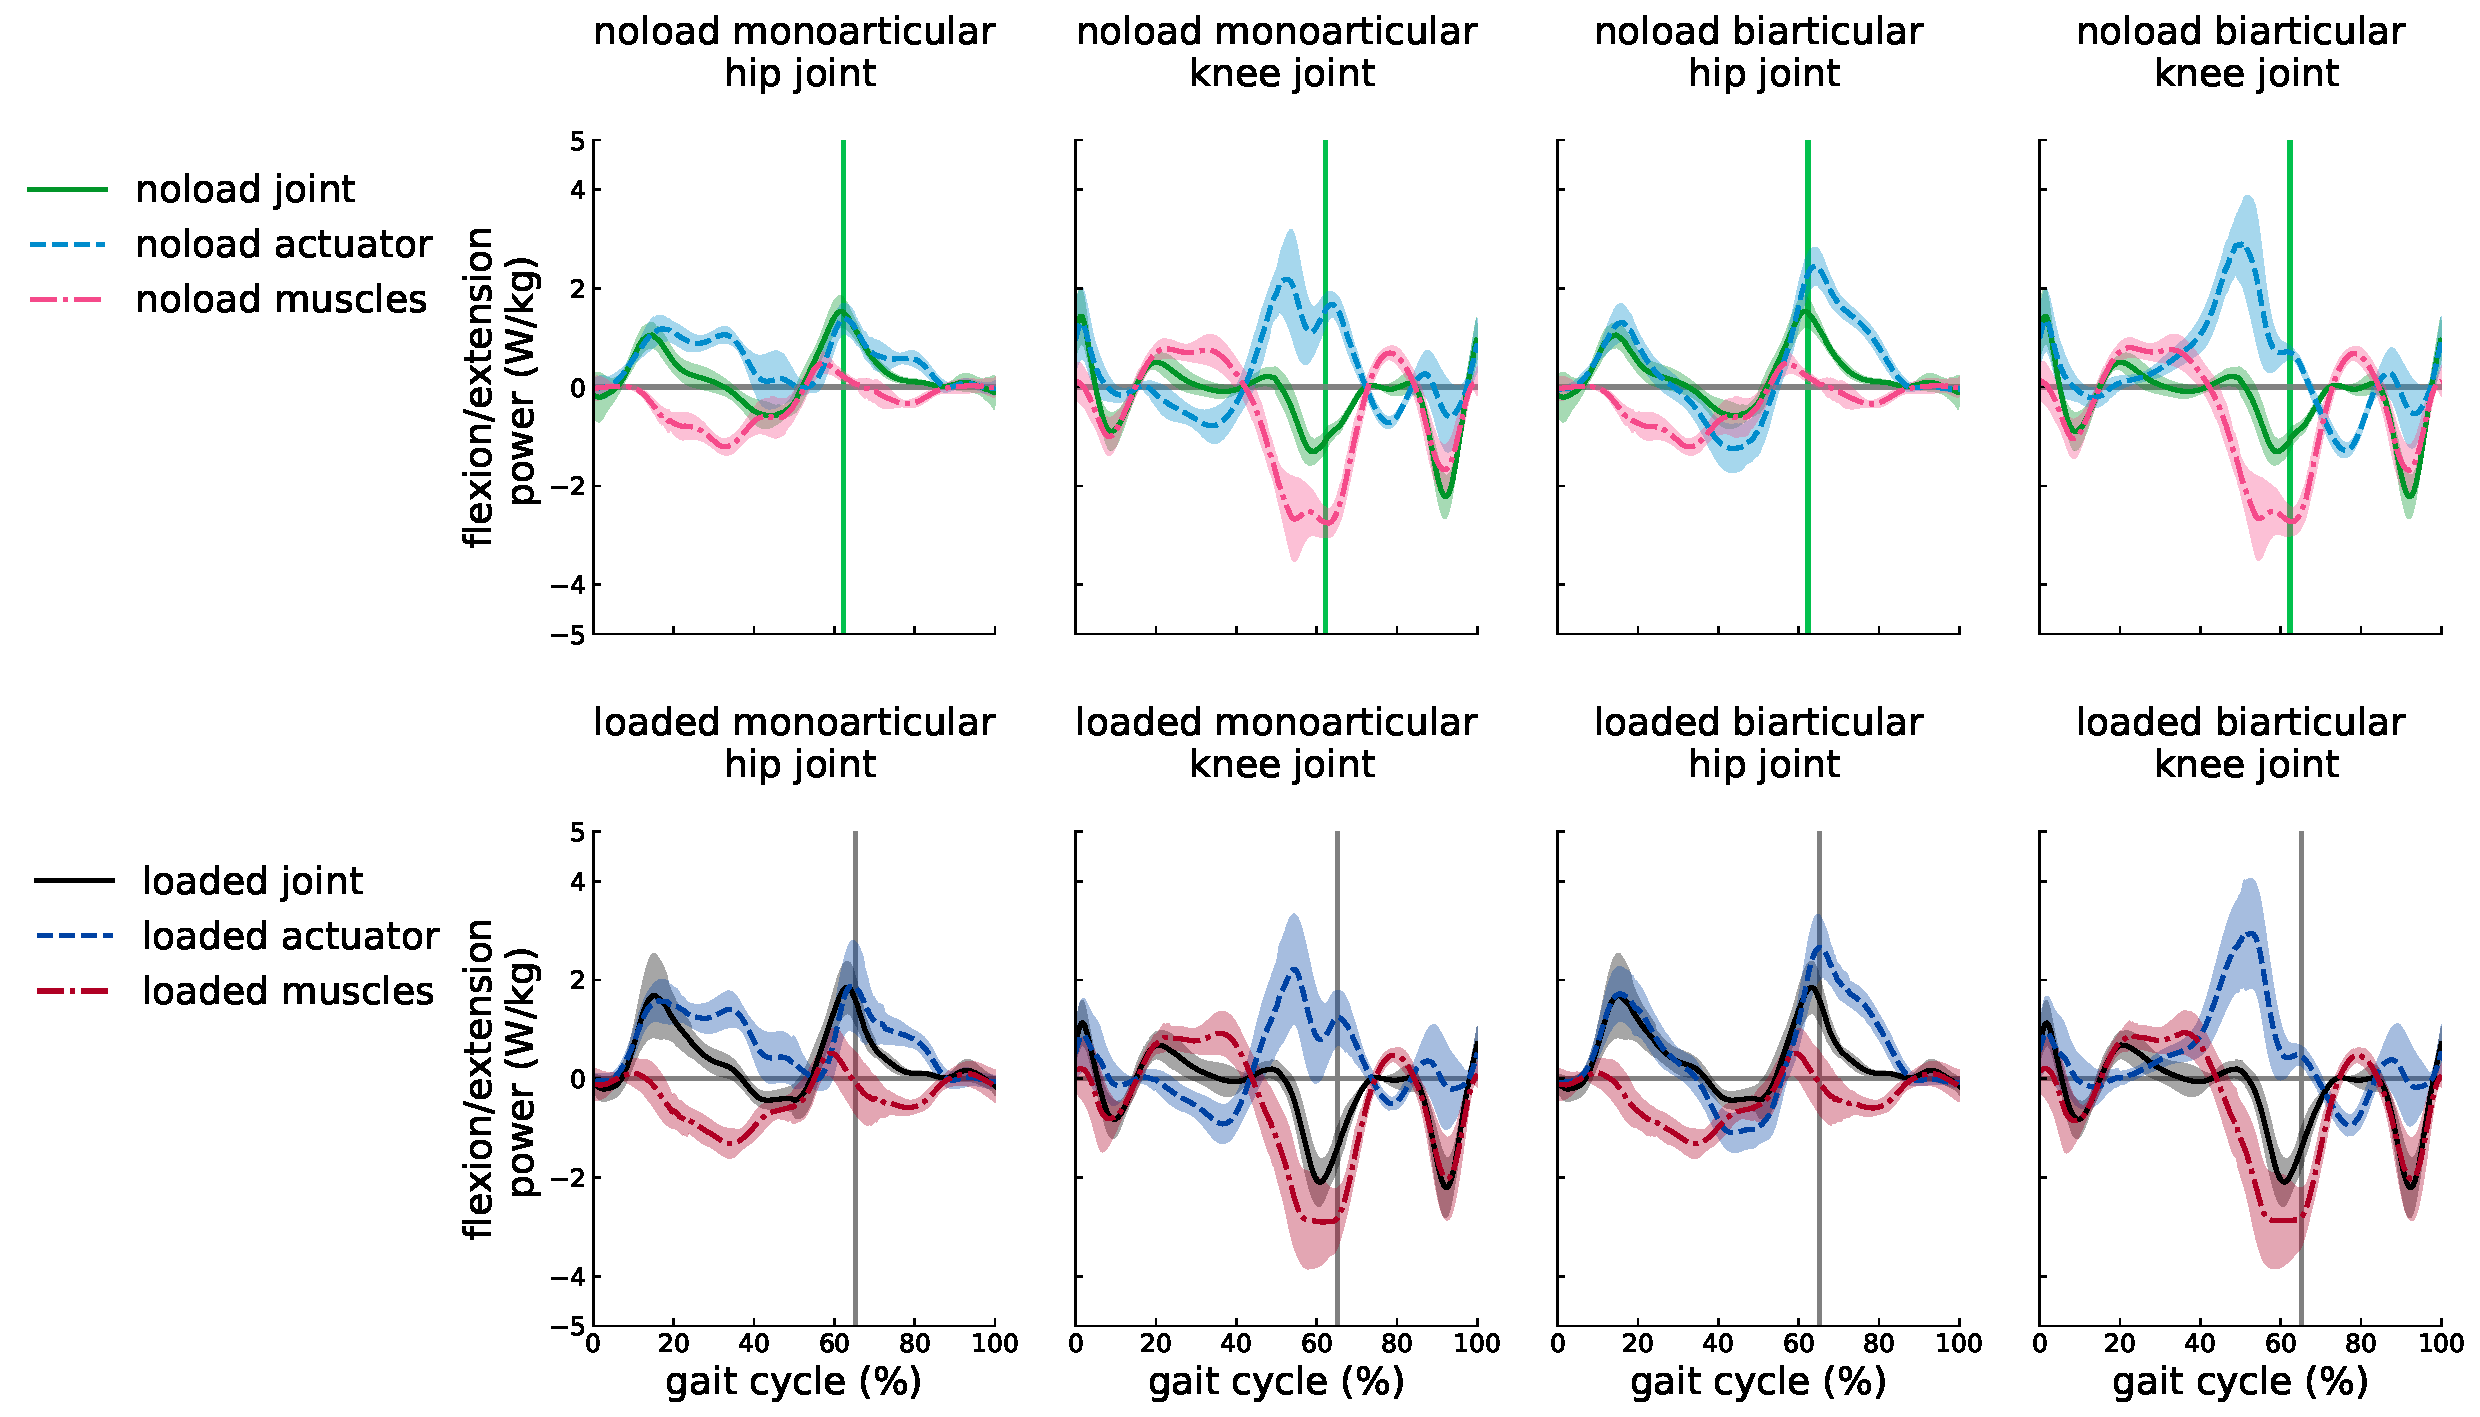
\includegraphics[width=\linewidth]{Ideal_Exo_MonovsBi_Figures/PaperFigure_Exoskeletons_Power.pdf}
	\vspace{1mm}
	\caption{{\small\textbf{Assistive devices power profiles compared to joint powers.} The device actuator power for subjects carrying heavy load (dark blue) and without any load (blue), and net joint power profile for \textit{loaded} (black) and \textit{noload} (green) conditions are shown for each actuator of the devices. The curves are averaged over 7 subjects with 3 trials and normalized by subject mass; shaded regions around the mean profile indicate standard deviation of the profile.}}
	\label{Fig_IdealExo_Power}
\end{figure*}
Due to the discussed kinematic differences between two configurations, the power profile of the exoskeletons were different in both actuators as it is represented in figure \ref{Fig_IdealExo_Power}. The magnitude of mechanical work performed by the biarticular actuators are higher than monoarticular mechanical work, and their profiles are different during the gait cycle except in the loading response and partially in mid-stance phases. The load carried by subjects causing different timing and magnitude than subjects walking with no load and the deviation of the profiles are higher for the \textit{loaded} subject, which both are observed in torque profiles as well.\\
Although the power profiles of hip actuators were roughly following the net joint power profile, the knee actuator profiles not resembled the knee joint power. The mechanical work performed by the assistive devices were mostly positive work for both knee and hip actuators. The negative mechanical work in the biarticular exoskeleton can be harvested mostly during the initial-swing and mid-swing phases for the knee actuator and terminal phase for the hip actuator. Unlike the biarticular device, the monoarticular hip actuator performed practically no negative mechanical work, and the regeneratable work of the knee actuator is within both mid-stance and late-swing phases.
%%%%%%%%%%%%%%%%%%%%%%%%%%%%%%%%%%%%%%%%%%%%%%%%%%%%%%%%%%%%%%%%%%%%%%%%%%%%%%%%%%%%%%%%%
\subsubsection*{Device Effect on Subjects Muscles}
\begin{figure*}[ht!]
	\centering
	\subfloat[\small{biarticular muscles}]{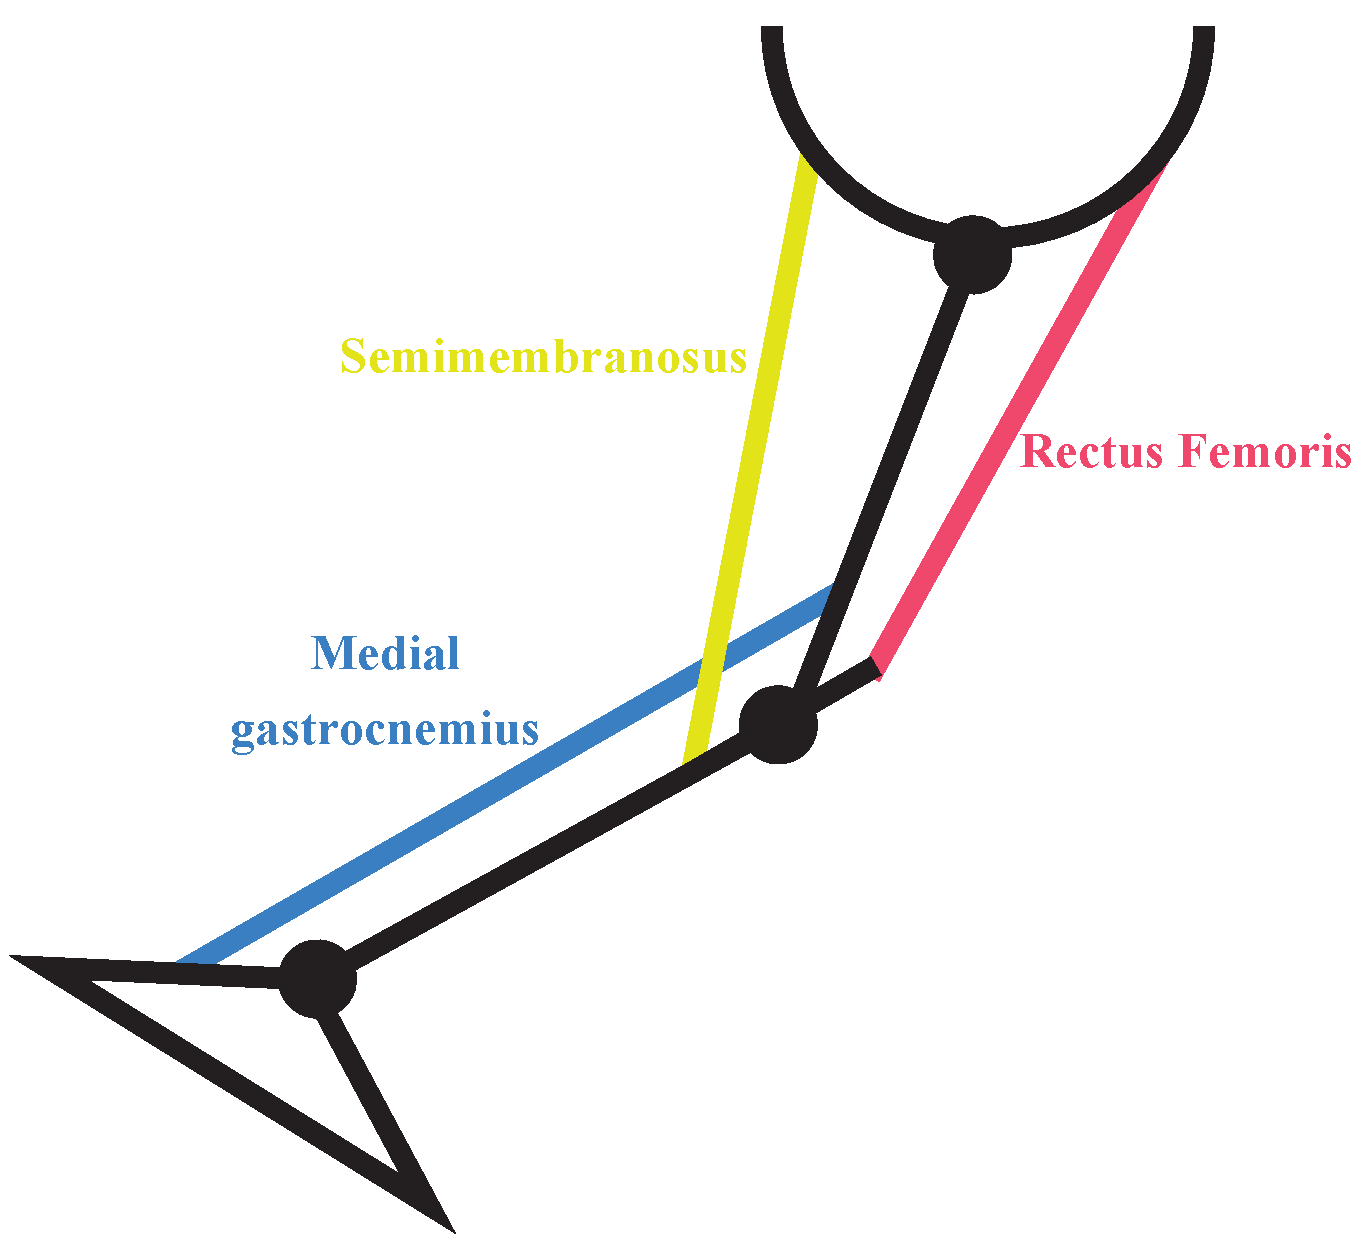
\includegraphics[width=2in]{Cartoons/Saggital_Leg_Biarticular_Muscles.pdf}
		\label{Fig_Bi_Muscles}}
	\hfil
	\subfloat[\small{monoarticular muscles}]{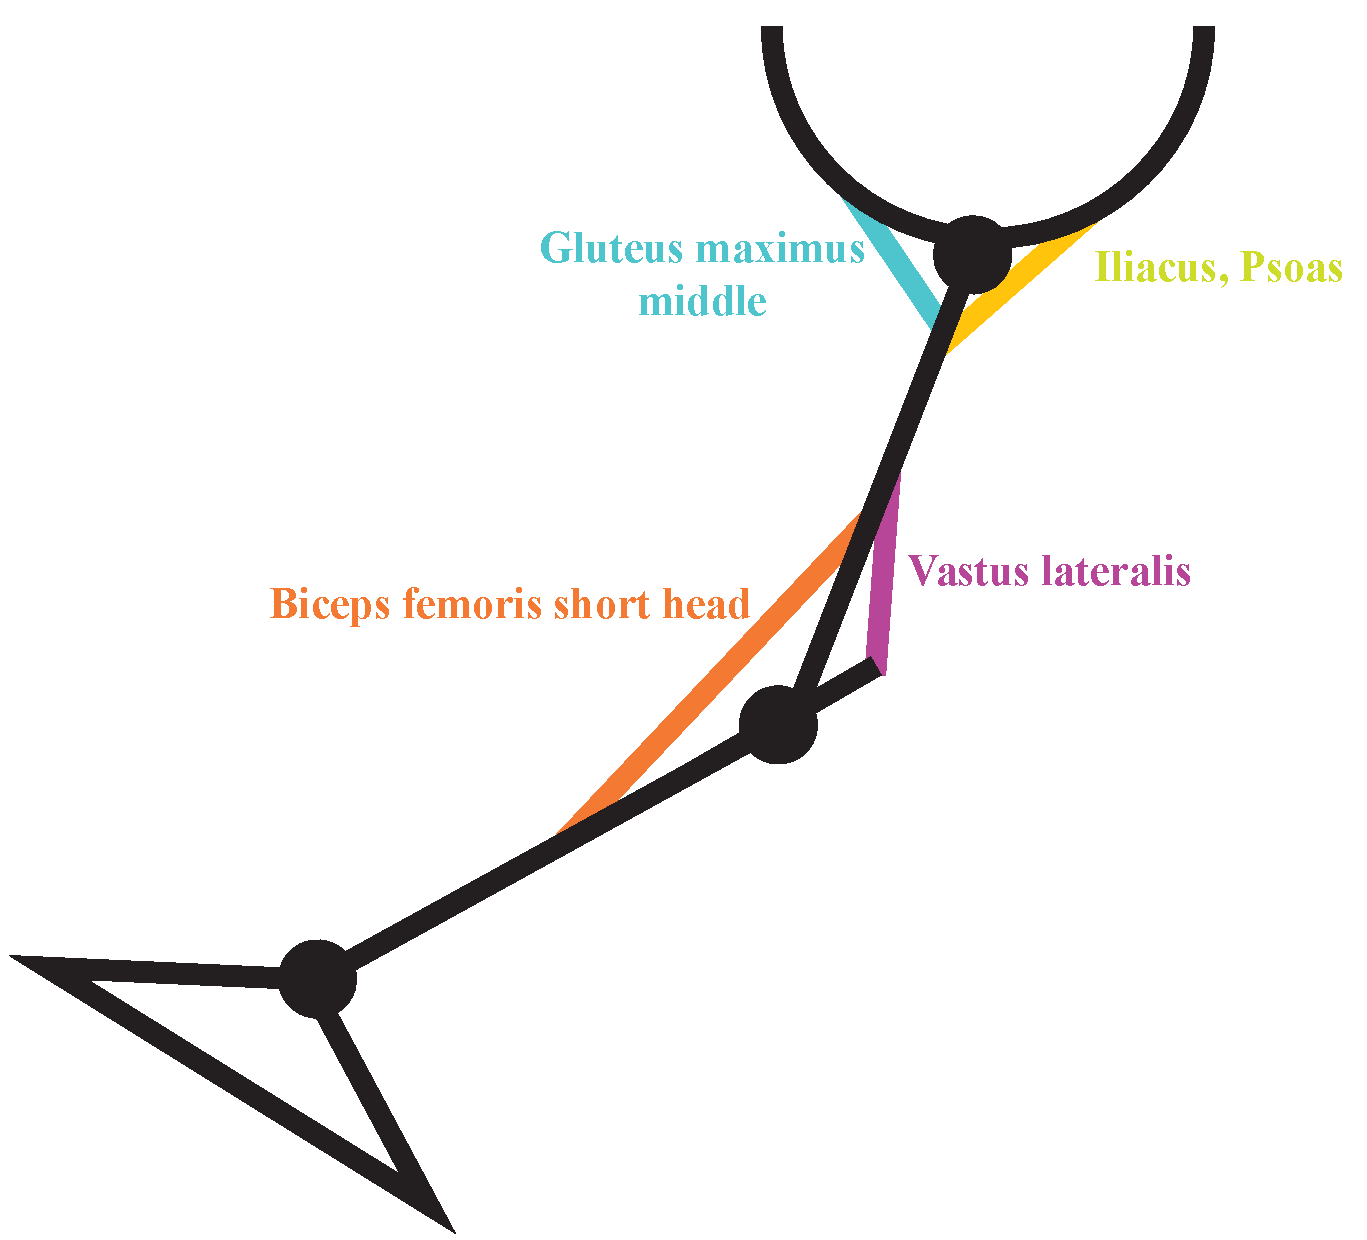
\includegraphics[width=2in]{Cartoons/Saggital_Leg_Monoarticular_Muscles.pdf}
		\label{Fig_Mono_Muscles}}
	\vspace{1mm}
	\caption{\small{\textbf{Biarticular and monoarticular representative lower extremity muscles}}}
	\label{Fig_Muscles}
\end{figure*}
\begin{figure*}[ht]   
	\centering
	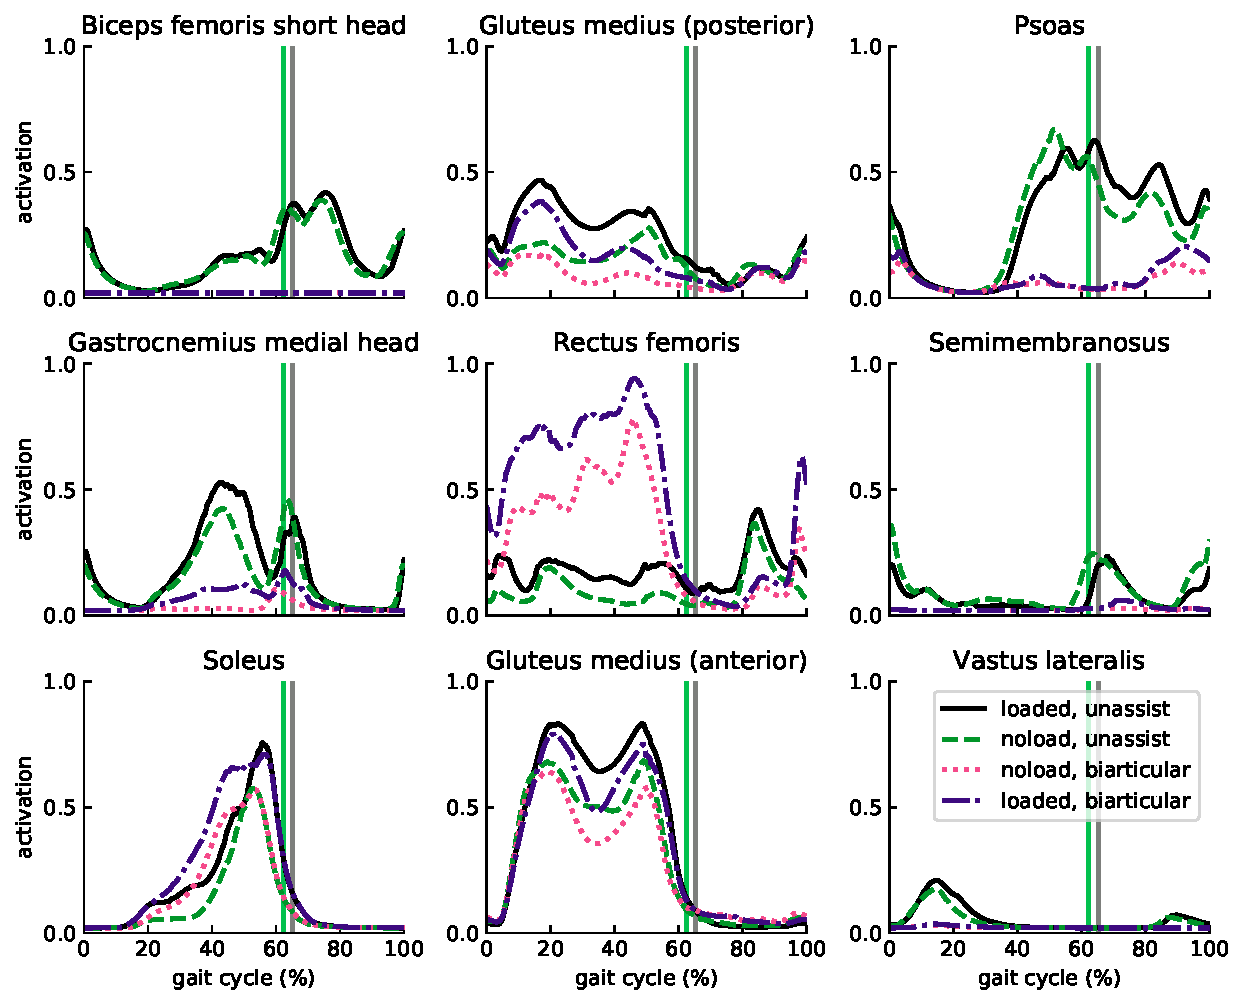
\includegraphics[width=\linewidth]{Ideal_Exo_MonovsBi_Figures/PaperFigure_Biarticular_MuscleActivation.pdf}
	\vspace{1mm}
	\caption{{\small\textbf{Activation of representative lower limb muscles of assisted and unassisted subjects.} The activation of unassisted subjects carrying heavy load (black) and without any load (green), and assisted subjects in \textit{loaded} (dark violet) and \textit{noload} (pink) conditions are shown for nine important muscles. The curves are averaged over 7 subjects with 3 trials.}}
	\label{Fig_IdealExo_MusclesActivation}
\end{figure*}
The muscular activation of the subjects assisted by ideal assistive devices has been considerably altered. Appending a set of ideal actuators with high optimal force (i.e., low penalization) to the musculoskeletal model changes the solution of the optimizer for finding a set of actuators to track the kinetics and kinematics of the joints.\\
The effect of appending ideal actuators not necessarily decreases the activity of all muscles, and it can be more economical for the complete set of actuators to increase the activity of specific muscles during some phases of gait to decrease the activity of less cost-effective muscles. Since metabolic power of muscles is a function of their activity, and their fiber properties \cite{106}, the reduction in the activity of the entire set of muscles is resulting in gross whole-body metabolic cost reduction.\\
Despite the kinematic difference between the two configurations of the assistive device, the applied torques to the joints are practically identical, and it resulted in an identical effect on the muscular activation of the subjects.\\
The reason for this issue rooted in the ideal nature of the actuators and devices, meaning that there are no constraints on the torque actuators can provide, the devices are assumed to be massless, and actuators do not have any reflected inertia effect. The muscle activation in figure \ref{Fig_IdealExo_MusclesActivation}, which is showing the effect of the biarticular device on the activation of representative muscles, is sufficient and can be generalized for both configurations of the assistive device. \\
The devices affected the activity of muscles throughout the lower extremity. This effect was significant on the Bicep femoris short head, Semimembranosus, and vasti muscles, where their activation has been replaced by another set of actuators, including muscles and ideal actuators.  The rectus femoris, which is a large knee extensor and hip flexor biarticular muscle,  activity has been considerably increased during the stance phase. This occurred so that the optimizer could take advantage of the rectus femoris high force-generating capacity to exert hip flexion and knee extension moments more economically. In the meanwhile, this high muscular activity of the rectus femoris resulted in high knee extension and hip flexion moments exceeding net joint moment of the joints that have been neutralized by ideal actuators, which are extremely economical for applying high torques due to its high optimal force assignments.\\
This set of activation in which hip flexion and knee extension required moment could be applied by more cost-effective muscles and actuators resulted in a substantial reduction in the activity of psoas and iliacus muscles as two major hip flexor muscles and the vasti muscles (vastus lateralis, vastus intermedius, and vastus medialis) as knee extensor set of muscles. The semimembranous muscle is another biarticular muscle contributing to hip extension and knee flexion moments, which has been affected by the assistive devices, and the new set of actuation has practically replaced its activity. The medial gastrocnemius as a critical knee flexor and ankle plantar flexor muscle has been affected by the assistive devices in which its activity has been substantially reduced, yet the muscle remained partially active to supply an ankle plantarflexion moment. The reduction of ankle plantarflexion moment has been compensated by increasing the activity of soleus as another primary ankle plantarflexor muscle. The assistive devices affected the activity of the gluteus medius muscles as well, which are not only responsible for a large fraction of hip abduction moment, but also they contribute to hip motion in the sagittal plane as well and hip rotation.\\
The anterior and posterior portions of the gluteus medius muscle, besides their primary contribution to hip abduction, were supporting the hip extension and flexion and its lateral and medial rotations. However, the contribution of thiese muscles to the hip sagittal moment replaced by assistive devices and a modified set of activations in assisted subjects, and it resulted in their muscular activity reduction.\\
The main differences between the muscular activity of the subjects walking normally and subjects walking while carrying a heavy load on torso are the magnitude and timing of the muscular activations which were observed already in other profiles as well. This load condition affected partially some muscles like Semimembranosus in which the device did not completely replaced by the ideal devices.
%%%%%%%%%%%%%%%%%%%%%%%%%%%%%%%%%%%%%%%%%%%%%%%%%%%%%%%%%%%%%%%%%%%%%%%%%%%%%%%%%%%%%%%%%
\subsection*{Pareto Simulation Results}
The assistive devices analyzed in the previous section, and their effect on metabolic cost and muscular activation of the subjects in two different load conditions have been studied. The simulations of the previous section were performed under the assumption that the assistive actuators have no bounds on the amount of the moment they can supply to the musculoskeletal model. However, this assumption is not a descriptive assumption for the real-time designing and controlling assistive device because the devices and especially untethered exoskeletons have some constraints on the amount of moment that their actuation unit can provide to assist the joint of interest and the suppliable energy from the battery for untethered exoskeletons is limited by the battery life. \\
One of the main aims of Pareto simulations was addressing this limitation through a simulation-based study in which we can analyze the performance of assistive devices under the limitation of their actuators on providing torque to the joints. 
The study has been accomplished by constraining the peak torque the assistive actuators can provide, and the optimal trade-off between the metabolic cost reduction and energy consumption of the devices has been obtained. The average Pareto front for the biarticular and monoarticular exoskeletons for both loading conditions of the subjects are represented in figure \ref{Fig_Main_Paretofronts}.\\
\begin{figure*}[ht]   
	\centering
	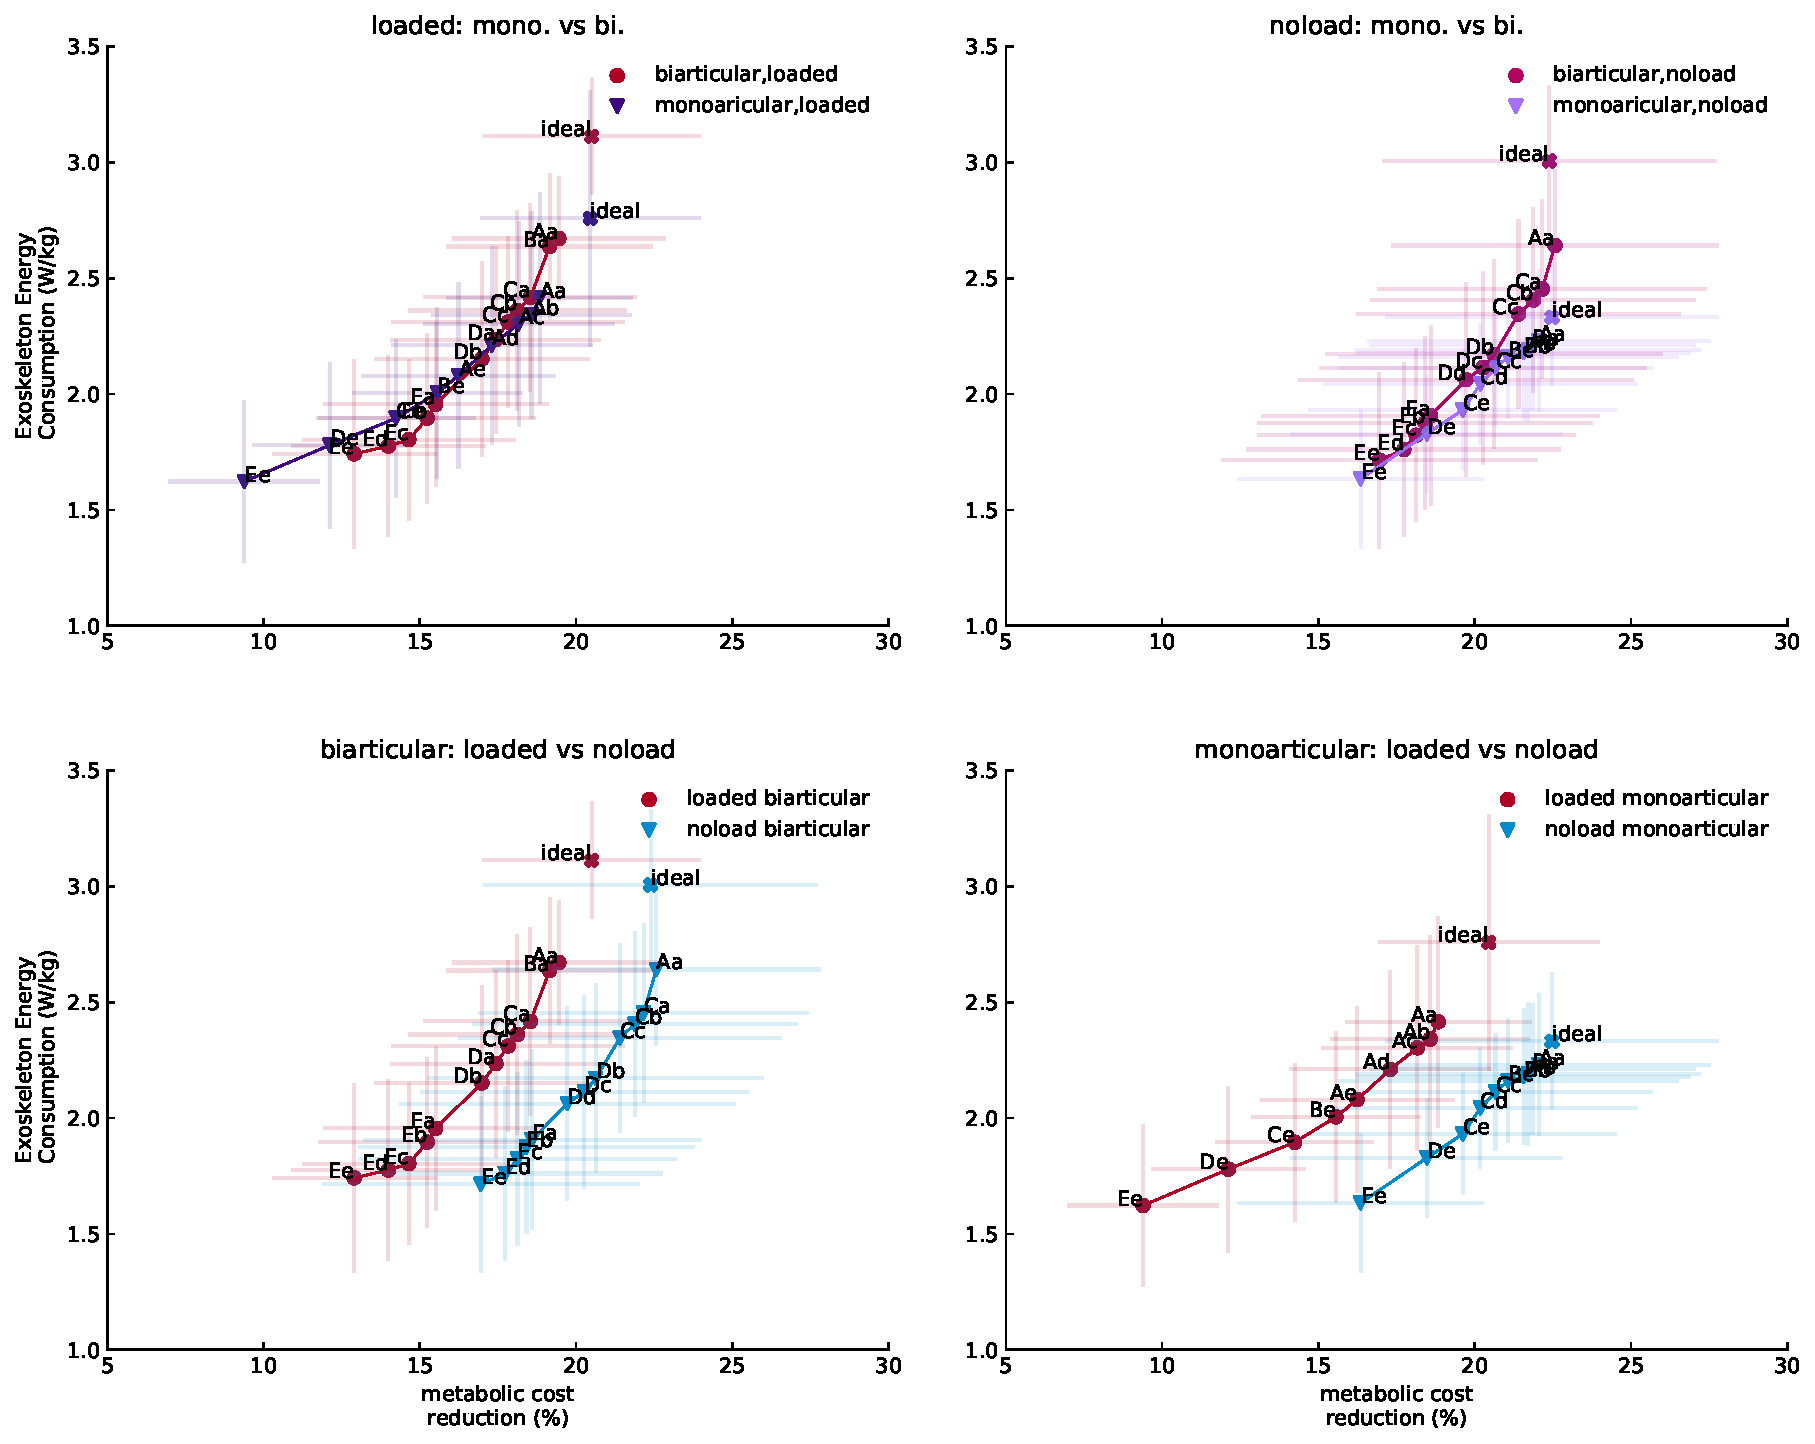
\includegraphics[width=\linewidth]{Pareto_Simulations_Figures/PaperFigure_Main_Pareto.pdf}
	\vspace{1mm}
	\caption{{\small\textbf{Optimal trade-offs between metabolic cost reduction and device energy consumption.} The numbering on each marker denotes results from different peak torque constraints. The hip and knee constraints are numbered from 1 to 5 in which 1 to 5 stand for 70 N.m to 30 N.m respectively, and each marker, which stands for a specific configuration of a device, is numbered by iterations of hip and knee constraints numbers. The optima points on Paretofronts are resulted from averaging over 7 subjects.}}
	\label{Fig_Main_Paretofronts}
\end{figure*}
\begin{figure*}[ht]   
	\centering
	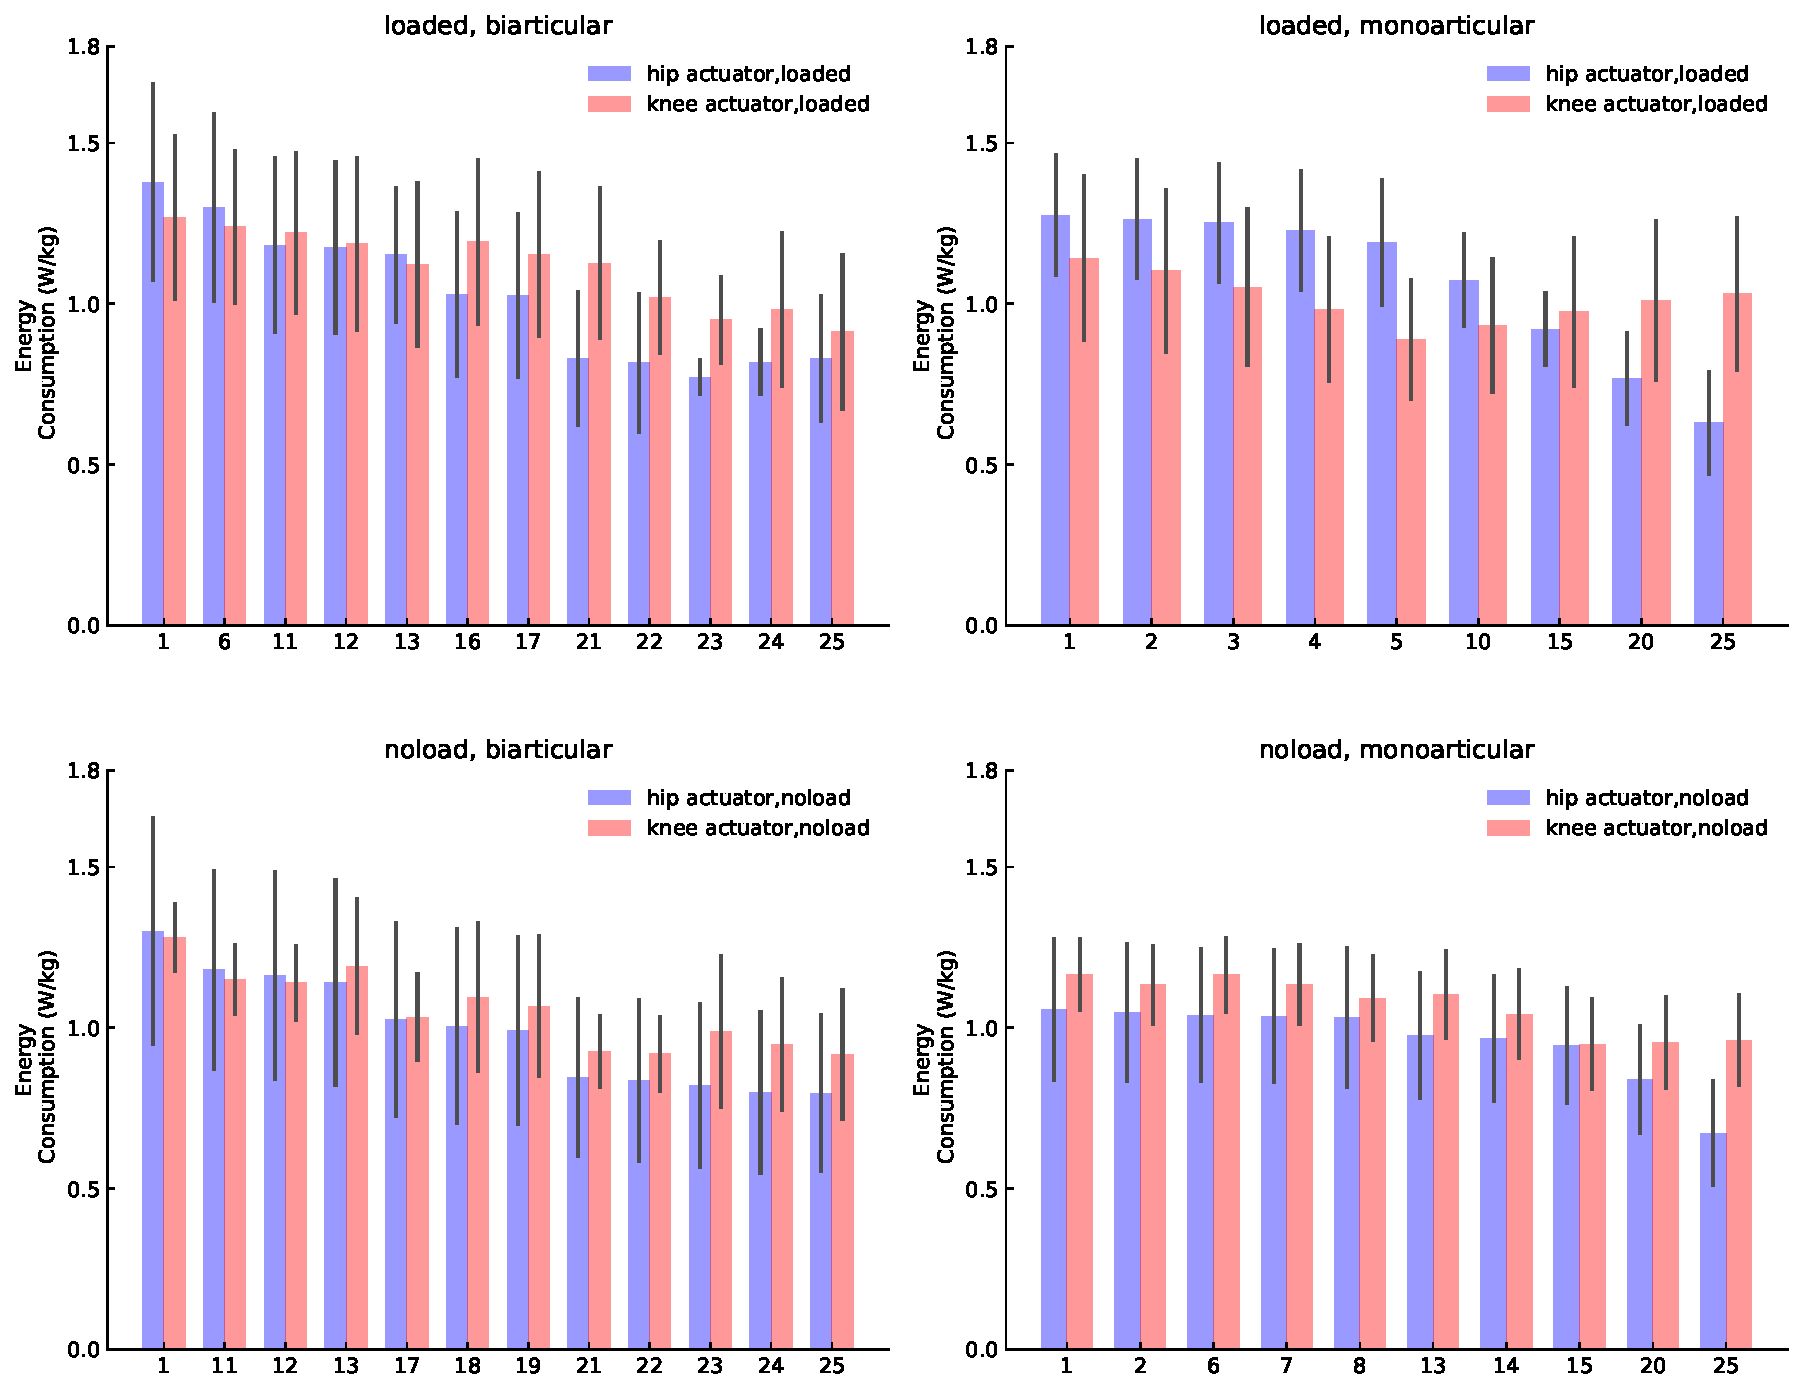
\includegraphics[width=\linewidth]{Pareto_Simulations_Figures/PaperFigure_Paretofront_EnergyBarPlot.pdf}
	\vspace{1mm}
	\caption{{\small\textbf{Energy consumption of optimal assistive actuators}. The horizontal axis shows the device number on the optimal pareto-front. The vertical lines represent the standard deviation of devices in 7 subjects.}}
	\label{Fig_Paretofronts_Actuators_EnergyBarPlot}
\end{figure*}
One of the immediate implications these Pareto fronts are providing is that the constrained devices in their maximum torque bounds where hip and knee restricted to 70 N.m peak torque, can mostly provide assistance that has been provided by the ideal exoskeletons with lower energy consumption in both load conditions (Table \ref{Table_Device_Performance_Comparison}).  Both constrained devices were able to assist the \textit{noload} subjects as much as the ideal exoskeletons were assisting, whereas the energy consumption in the biarticular exoskeleton was reduced considerably reduced compared to its ideal actuation, but the monoarticular energy consumption was practically the same with its ideal configuration.\\
Similar to the \textit{noload} condition, the constrained devices had a high metabolic reduction in the \textit{loaded} subjects; even though it was not the same with the ideal configuration of the devices, the energy consumption had a considerable reduction, especially in the biarticular configuration which is the same as the \textit{noload} condition.
The performance of devices under peak torque limitation and its comparison with the ideal devices implies that the comparison of assistive devices with unlimited actuation units is not a legitimate comparison suggesting that the comparison between assistive devices should be conducted using optimal trade-off points of devices in which a device has its optimal performance in both energy consumption and metabolic cost reduction criteria.\\
\begin{table}[ht]
	\centering
	\renewcommand{\arraystretch}{1.2}
	\begin{adjustwidth}{-2.2in}{0in}
	\caption{\small{\textbf{Device performance in with ideal and constrained actuators.}}}
	\begin{tabular}{c!{\vline width 0.2pt}c!{\vline width 0.2pt}c!{\vline width 0.2pt}c!{\vline width 0.2pt}c!{\vline width 0.2pt}c}
		\toprule
		\multirow{2}{*}{\textbf{configuration}} & \multirow{2}{*}{\textbf{device type}} & \multirow{2}{*}{\textbf{condition}} & \textbf{hip energy}& \textbf{knee energy} & \textbf{metabolic cost}\\
		&  &  &\textbf{consumption (W/kg)} & \textbf{consumption (W/kg)} & \textbf{reduction (\%)} \\
		\midrule[0.75pt]
		\multirow{4}{*}{\textbf{biarticular}} & ideal & \textit{noload} & 1.42 $\pm$ 0.32 & 1.58 $\pm$ 0.30 & 22.38 $\pm$ 4.91 \\
		\cmidrule[0.2pt]{2-6}
		& ideal & \textit{loaded} & 1.58 $\pm$ 0.29 & 1.52 $\pm$ 0.29 & 20.49 $\pm$ 2.87 \\
		\cmidrule[0.2pt]{2-6}
		& constrained  & \textit{noload} & 1.30 $\pm$ 0.36 & 1.28 $\pm$ 0.29 & 22.57 $\pm$ 4.92 \\
		\cmidrule[0.2pt]{2-6}
		& constrained  & \textit{loaded} & 1.38 $\pm$ 0.36 & 1.27 $\pm$ 0.29 & 19.54 $\pm$ 2.79 \\
		\midrule[0.75pt]
		\multirow{4}{*}{\textbf{Monoarticular}} & ideal & \textit{noload} & 1.09 $\pm$ 0.24 & 1.24 $\pm$ 0.13 & 22.47 $\pm$ 4.89 \\
		\cmidrule[0.2pt]{2-6}
		& ideal & \textit{loaded} & 1.52 $\pm$ 0.28 & 1.24 $\pm$ 0.27 & 20.45 $\pm$ 2.81 \\
		\cmidrule[0.2pt]{2-6}
		& constrained  & \textit{noload} & 1.06 $\pm$ 0.22 & 1.16 $\pm$ 0.12 & 22.05 $\pm$ 5.18 \\
		\cmidrule[0.2pt]{2-6}
		& constrained  & \textit{loaded} & 1.27 $\pm$ 0.19 & 1.10 $\pm$ 0.26 & 18.68 $\pm$ 2.36 \\
		\bottomrule
	\end{tabular}%
	\label{Table_Device_Performance_Comparison}
	\end{adjustwidth}
\end{table}
The biarticular and monoarticular exoskeletons are showing practically similar performance in assisting subjects with and without load. Nevertheless, analyzing the energy consumption of the devices on the Pareto front reveal that the monoarticular device considerably affected by the load condition of subjects in which the performance of monoarticular exoskeleton became practically identical with the biarticular device when subjects were \textit{loaded} whereas the monoarticular device had superior performance in \textit{noload} condition.\\
The detailed analysis of the monoarticular device show that both actuators of this device were affected by loading subjects with a heavy load (figure \ref{Fig_Main_Paretofronts} and \ref{Fig_Paretofronts_Actuators_EnergyBarPlot}), and unlike the \textit{noload} condition where knee actuator energy consumption was dominant to the hip in all optimal devices, loading subjects increased the amount of mechanical work of performed by the hip. In contrast, the energy consumption of the biarticular knee and hip actuators was not affected noticeably by loading subjects as figure \ref{Fig_Paretofronts_Actuators_EnergyBarPlot} representing the energy consumption of optimal devices.Additionally, the optimal configurations of the biarticular exoskeleton are mostly similar in the subjects walking while carrying a heavy load and walking normally, whereas monoarticular exoskeleton has different configurations in both load conditions. The practically similar configurations and the performance of the biarticular exoskeleton in both load conditions can facilitate designing a biarticular device and and developing a generic controller to assist the subjects in different  load conditions.\\
\subsection*{Optimal device torque and power profiles }
\begin{figure*}[ht]   
	\centering
	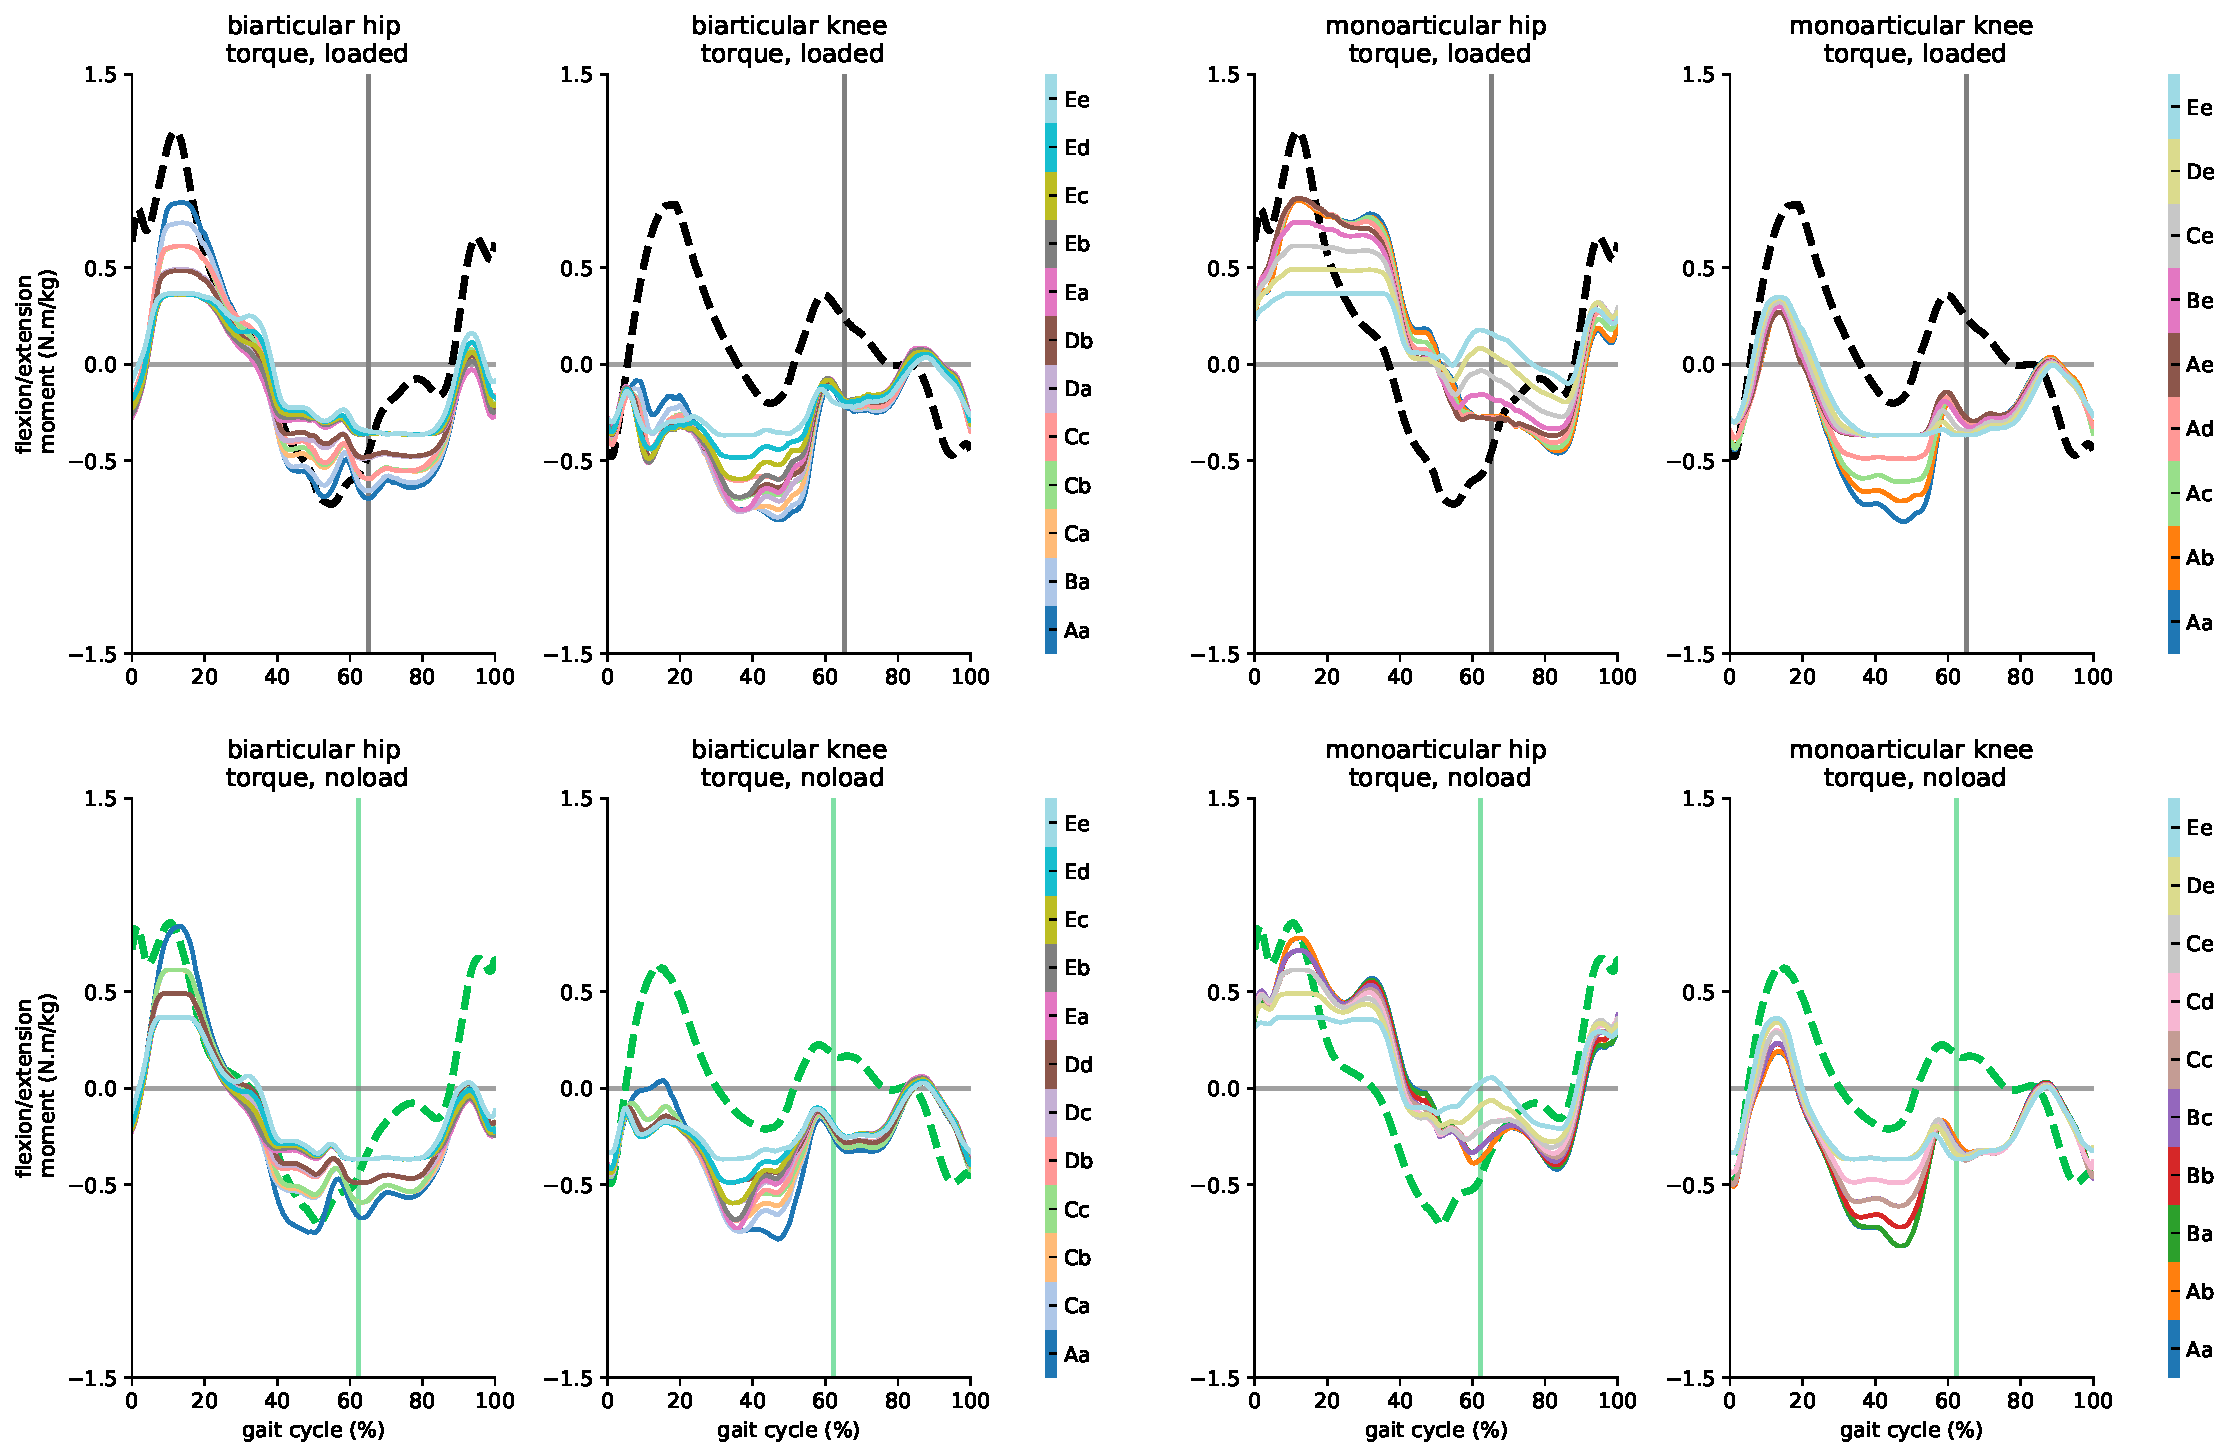
\includegraphics[width=\linewidth]{Pareto_Simulations_Figures/PaperFigure_Paretofront_TorqueProfiles.pdf}
	\vspace{1mm}
	\caption{{\small\textbf{Optimal assistive devices torque profiles compared to joint moments.} Each line represents the torque profile of a different optimal device defined in the color bar. The hip and knee constraints are numbered from 1 to 5 in which 1 to 5 stand for 70 N.m to 30 N.m, respectively, and the configuration of the optimal device has been specified by the number of each line that is computed by multiplication of hip and knee constraints numbers. The curves are averaged over 7 subjects with 3 trials normalized by subject mass.}}
	\label{Fig_Paretofronts_Torque_Profiles}
\end{figure*}
The torque profiles of constrained optimal devices slightly differed from the net joint moment of the hip, and the knee joints and the general torque trajectories of these actuators were mostly similar to the torque profiles of the devices with ideal actuators. The ideal and constrained torque profiles of biarticular hip actuators had mostly magnitude differences during mid-stance and terminal-stance to terminal-swing phases. In contrast to the hip actuator, the knee actuator has practically the same profile with the ideal knee actuator during the swing phase, but the path and magnitude of the knee actuator were mostly different from the ideal device. This comparison between the ideal and constrained devices is mostly valid when subjects were walking without carrying any load, and the only difference was the magnitude of the constrained profiles.\\
Both actuators of the constrained monoarticular device have different profiles with the ideal device. The hip actuators had a significant magnitude difference during the load response phase, and most of the optimal constrained hip actuators were saturated during mid-stance and terminal stance phases, which was affecting the trajectory as well. The difference between hip actuators became highly significant during pre-swing to mid-swing phases, where the torque trajectories of the constrained hip actuator were not only different from the ideal actuator but also there was high variation among optimal constrained actuators. The monoarticular knee had more resemblance to the ideal knee actuator torque profile where they had practically identical profiles during the swing phase, and the difference between them was the higher torque magnitude during the mid-stance and lower magnitude during the pre-swing phases. Unlike the biarticular exoskeleton, where the load condition had only effect on the magnitude of the profiles, and there was a close similarity between the torque trajectories in \textit{loaded} and \textit{noload} conditions, the hip actuator torque of the monoarticular device assisting the subjects walking without carrying any load had considerable differences with the \textit{loaded} condition device. These two profiles had two mostly different trajectories and magnitudes during all phases of a gait cycle, and their differences are more unambiguous during load response to mid-swing phases.\\
\begin{figure*}[ht]   
	\centering
	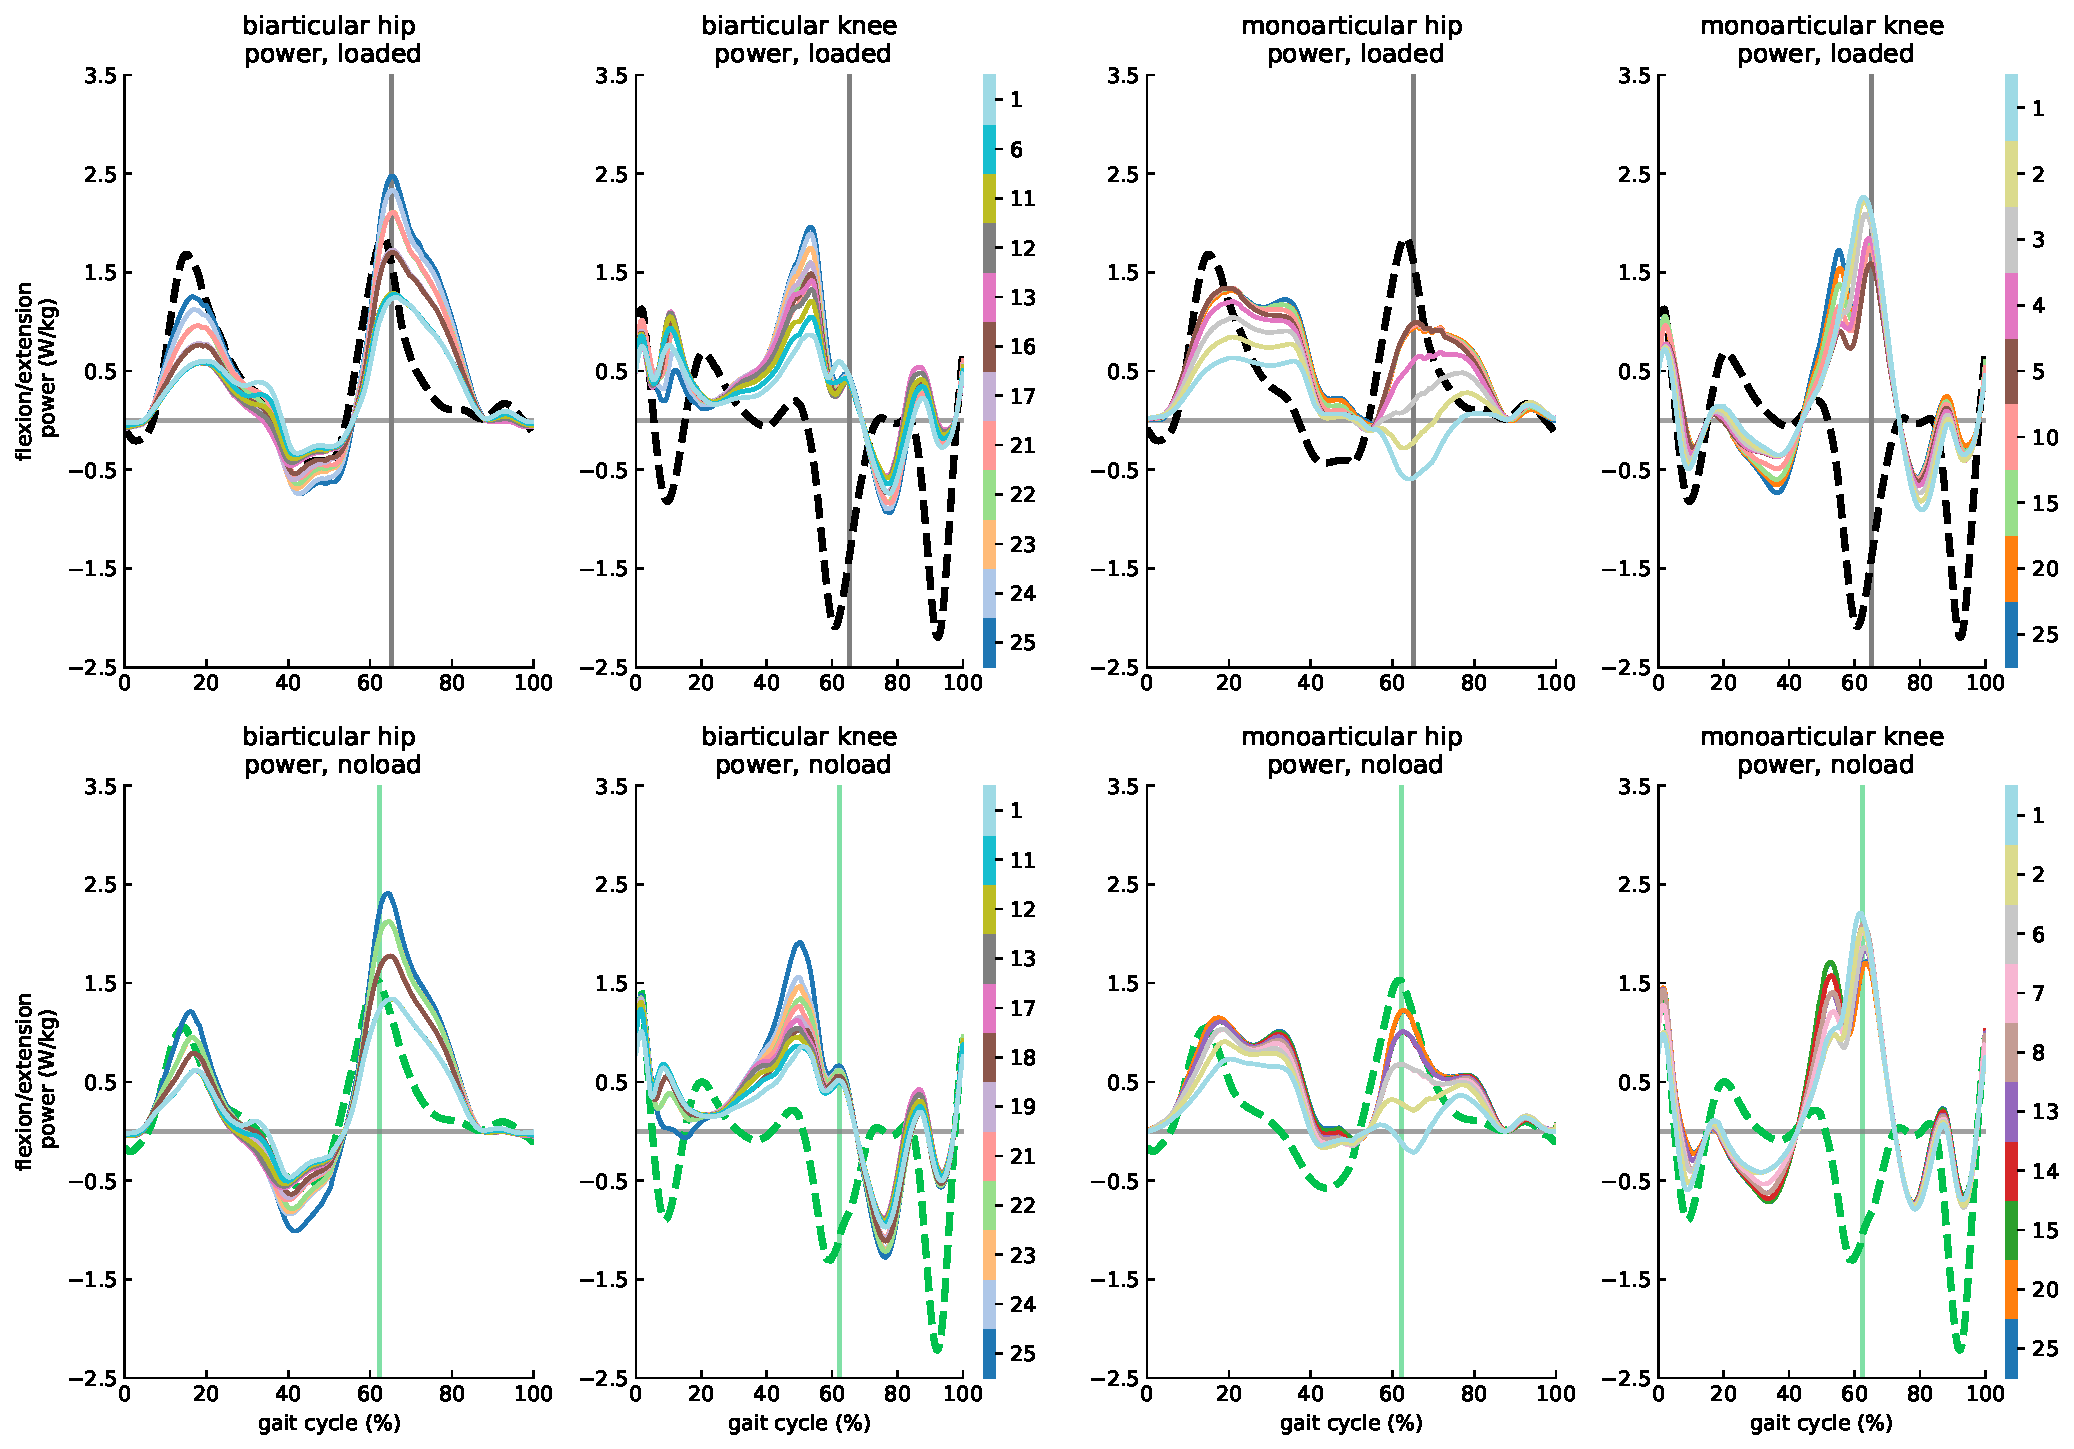
\includegraphics[width=\linewidth]{Pareto_Simulations_Figures/PaperFigure_Paretofront_PowerProfiles.pdf}
	\vspace{1mm}
		\caption{{\small\textbf{Optimal assistive devices power profiles compared to joint power.} Each line represents the power profile of a different optimal device defined in the color bar. The hip and knee constraints are numbered from 1 to 5 in which 1 to 5 stand for 70 N.m to 30 N.m, respectively, and the configuration of the optimal device has been specified by the number of each line that is computed by multiplication of hip and knee constraints numbers. The curves are averaged over 7 subjects with 3 trials normalized by subject mass.}}
	\label{Fig_Paretofronts_Power_Profiles}
\end{figure*}
The restrained biarticular and monoarticular devices had a resemblance to the ideal devices similar to the torque profiles similarity to ideal profiles. The biarticular hip actuator has mostly a similar power trajectory for the hip in both load conditions with considerably lower magnitude for all optimal devices where this magnitude difference is more substantial during mid-stance and initial swing to mid-swing phases; while the knee actuator has a high correlation with the ideal actuator, the loading response and mid-stance phases of the constrained knee actuator is different with the ideal actuator like the torque profile. The constrained monoarticular hip actuator has a high variation within optimal devices, and most of the optimal configurations have their unique power profile; nevertheless, the optimal devices with the highest peak torque limitations have a close resemblance to the ideal device. In contrast to the hip actuators, the power trajectories of the knee actuator in both load conditions were similar to the ideal device with a difference during pre-swing to mid-swing phases where the peak power consumption occurs about the toe-off in the constrained knee actuators.\\
The power and torque profiles of optimal biarticular and monoarticular devices revealing that although the optimal monoarticular exoskeletons have a lower energy consumption comparing to the optimal biarticular devices, the variation of the torque and power profiles within optimal configurations of the monoarticular device is higher than biarticular devices and load condition of the subjects can considerably affect the profiles of assistive actuators. These variations within optimal monoarticular devices indicate that achieving a generalized design and control policies for assisting subjects in different load conditions and different actuation and battery life limitations would be genuinely challenging with monoarticular exoskeletons.\\

\subsection*{Mass, inertia and regeneration effects}
\begin{figure*}[ht]   
	\centering
	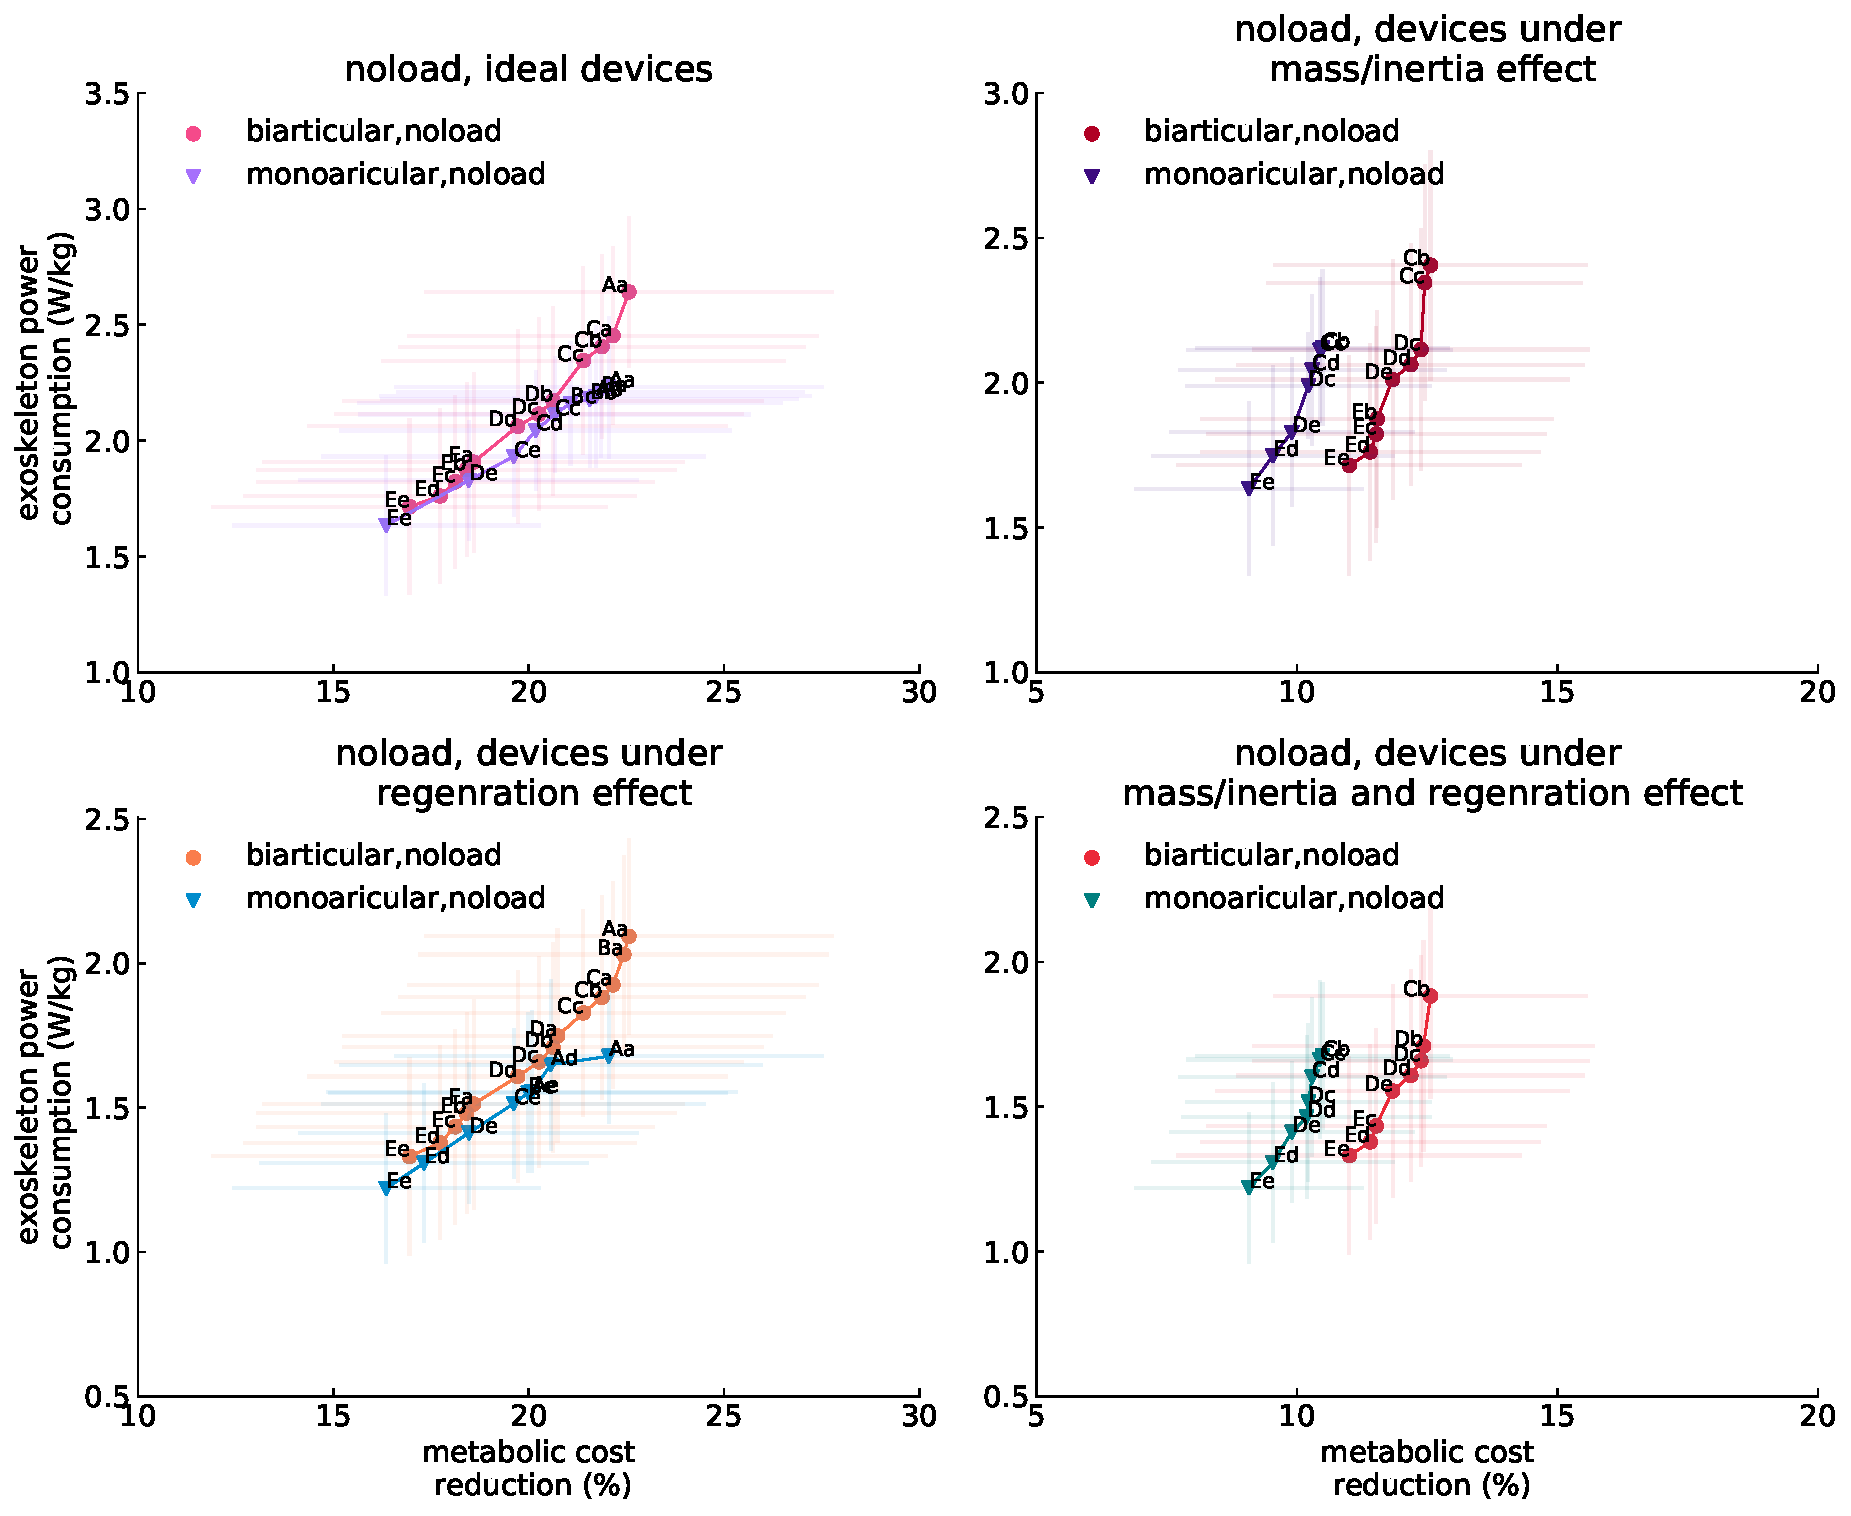
\includegraphics[width=\linewidth]{Pareto_Mass_Regenration_Figures/PaperFigure_AddingMass_Pareto.pdf}
	\vspace{1mm}
	\caption{{\small\textbf{Optimal assistive devices power profiles compared to joint power.} }}
	\label{Fig_Paretofronts_Mass_Regeneration_Effect}
\end{figure*}
\begin{figure*}[ht]   
	\centering
	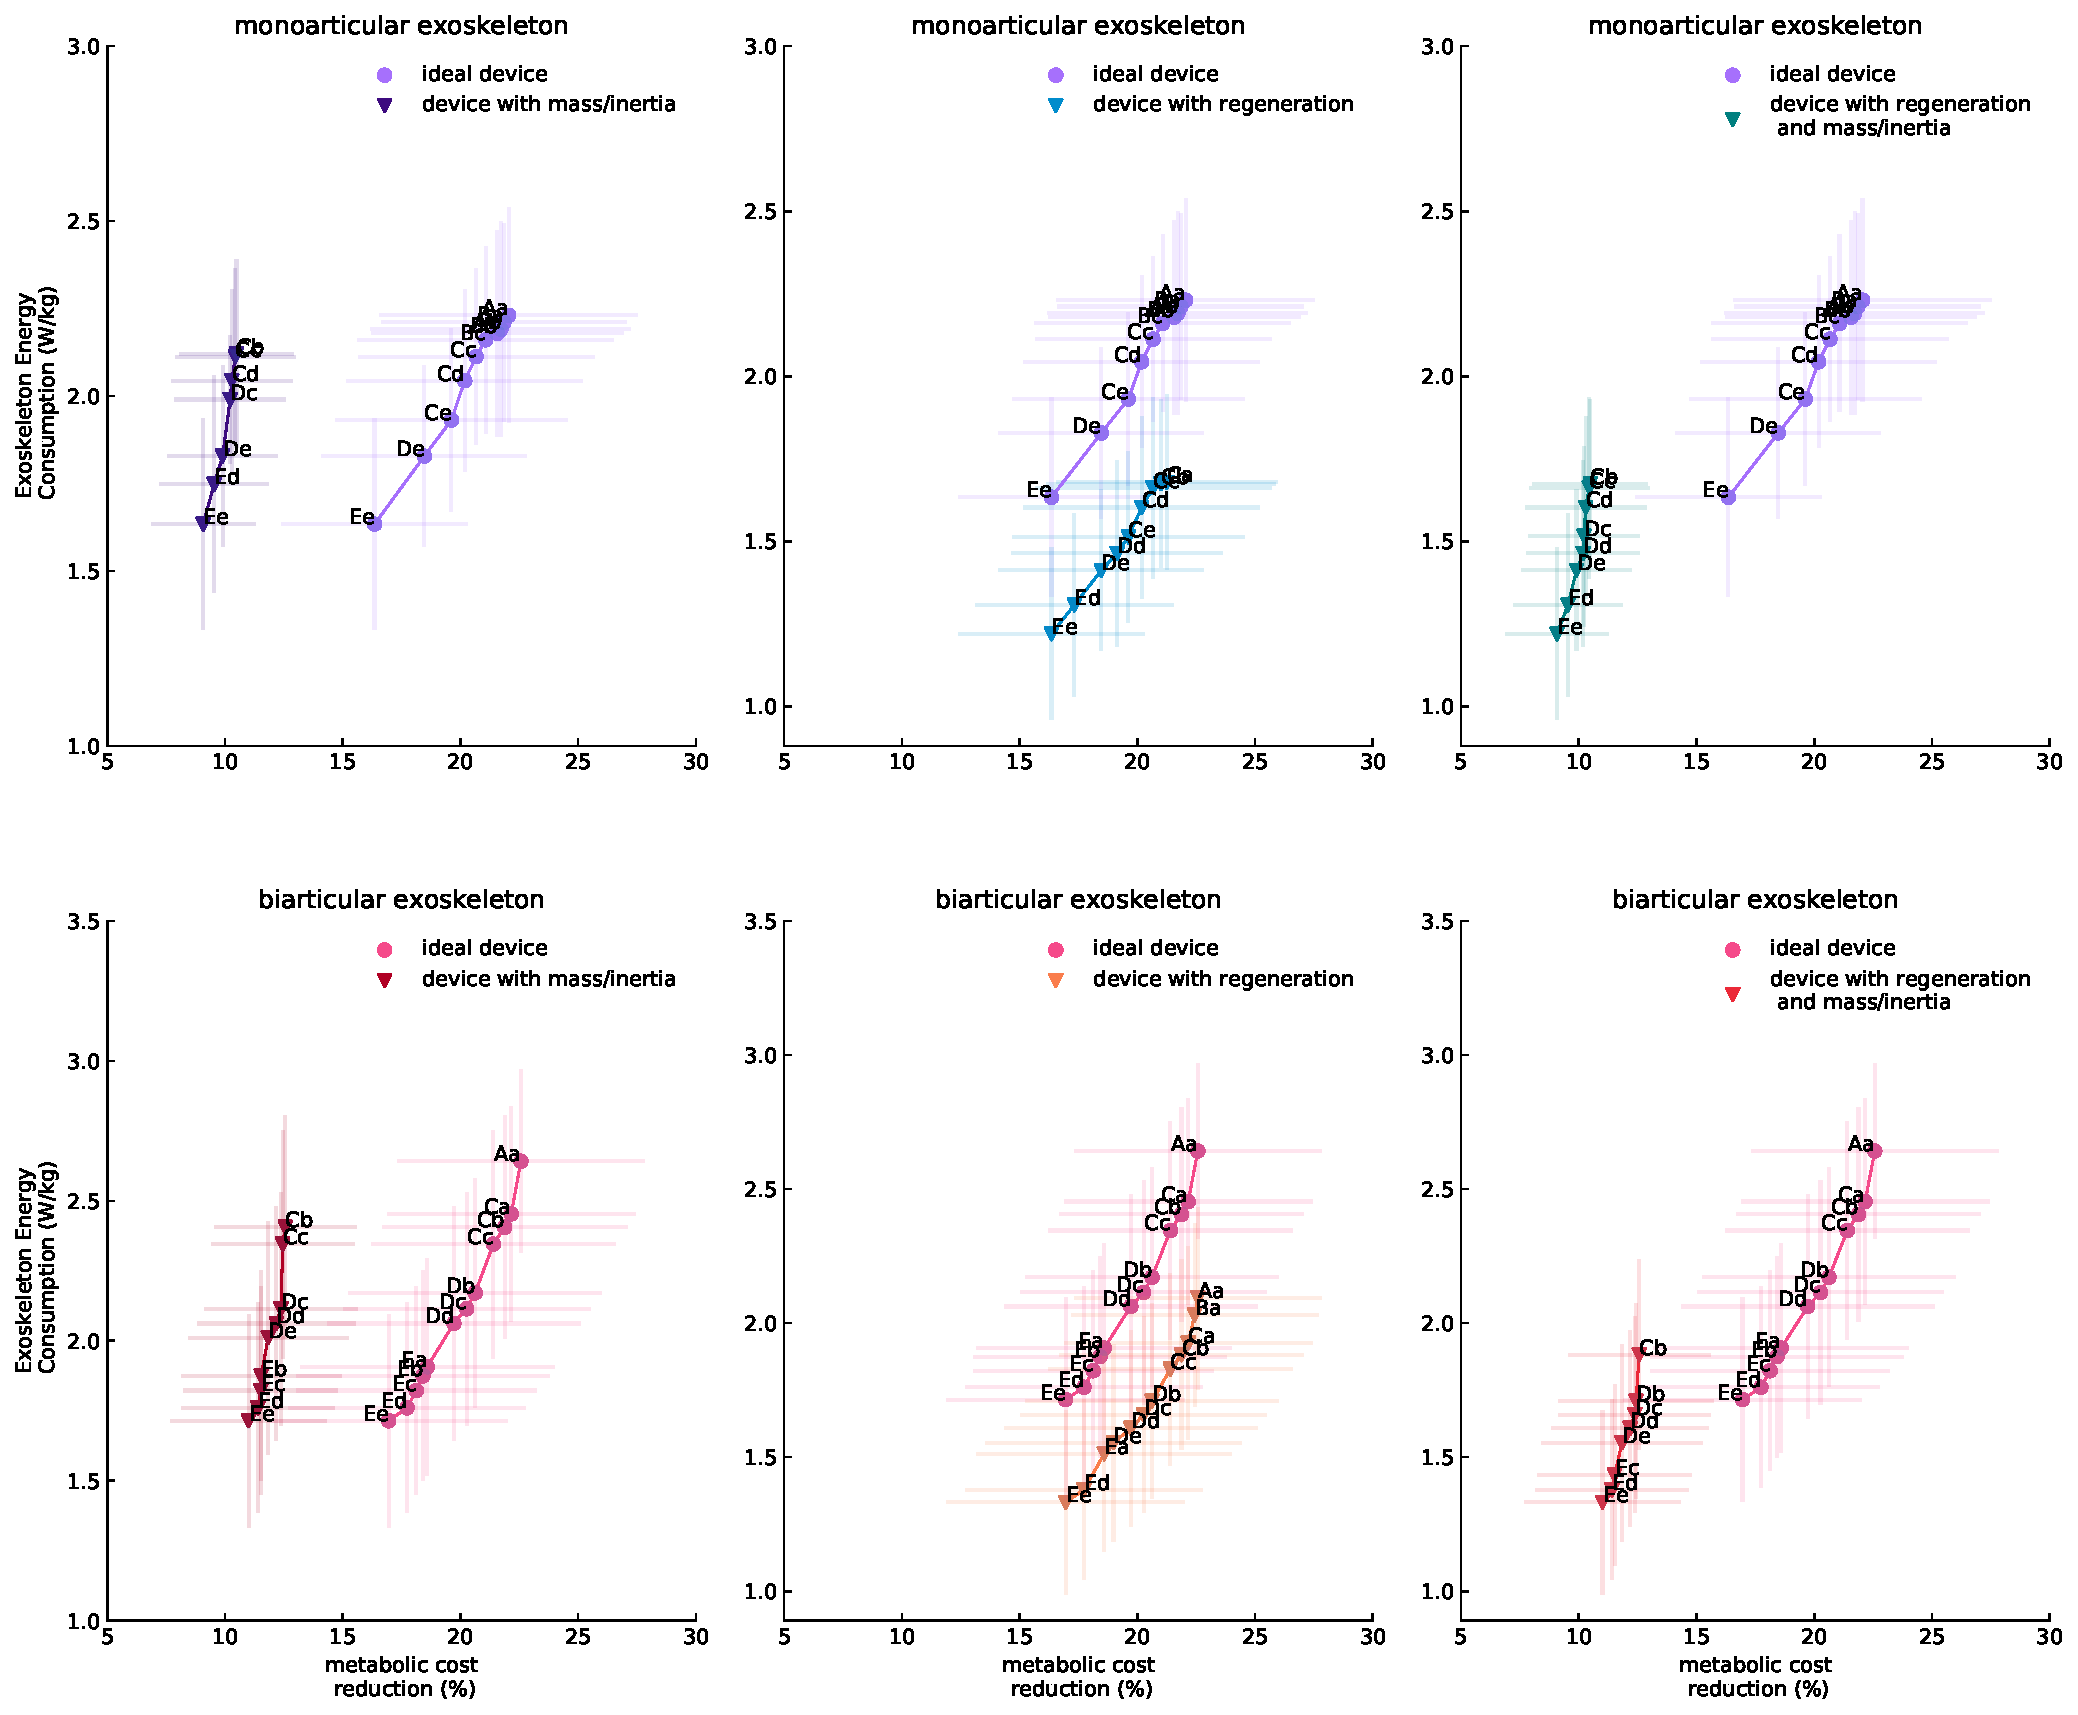
\includegraphics[width=\linewidth]{Pareto_Mass_Regenration_Figures/PaperFigure_Pareto_Comparison.pdf}
	\vspace{1mm}
	\caption{{\small\textbf{Optimal assistive devices power profiles compared to joint power.}}}
	\label{Fig_Paretofronts_Mass_Regeneration_Effect_Comparison}
\end{figure*}
\subsection*{Case Study}
We conducted four different case studies to get more insight into the performance of two assistive devices in a particular load condition or an assistive device in two different load conditions with the same effect on the metabolic energy expenditure or the same energy consumption of assistive actuators. Investigating these specific configurations of the optimal devices helps us understand how the profiles of devices with the same performances are changing in a load condition and what their effect is on muscle coordination. These cases can help to clarify the effect of load condition on an assistive device profiles, and their muscles and how a particular device will be affected by loading assisted subjects with a heavy load.
\subsubsection*{Case 1: Devices Performance in \textit{\textit{noload}} Condition} 
\subsubsection*{Case 2: Devices Performance in \textit{\textit{loaded}} Condition} 
\subsubsection*{Case 3: Biarticular Exoskeleton Performance} 
\subsubsection*{Case 4: Monoarticular Exoskeleton Performance}
%%%%%%%%%%%%%%%%%%%%%%%%%%%%%%%%%%%%%%%%%%%%%%%%%%%%%%%%%%%%%%%%%%%%%%%%%%%%%%%%%%%%%%%%%
\subsection*{Study Limitations}
This simulation-based studying assistive device has some limitations that need to be considered for any interpretation of the results. One of the main limitations is kinematics and ground reaction forces for the assisted subjects; Although experimental studies reported that exoskeleton could make a minor \cite{42,79,91,114,115,116} and significant \cite{80,117,118,119} changes on assisted subjects kinematics and joint moment, our simulator's algorithm (CMC) is not capturing these changes and it is assumed that unassisted and assisted subjects have the same kinematics, ground reaction force, and joint moment, nonetheless, it is reported that metabolic cost may not substantially be affected by kinematics changes\cite{120}. This limitation recently has been addressed by employing predictive simulations which can capture the changes in the kinematics and dynamics of the assisted subjects.\\  
Secondly, as it is earlier stated, assistive devices that we modeled was assumed massless without any actuator and link mass and inertia; yet, in practice, exoskeleton actuation modules mass and their reflected inertia on the links are large and one of the main challenges on mechanical design of the exoskeletons and also it is proven that adding mass the lower limbs can considerably change metabolic cost of the subjects. The exoskeletons attachment on the body is also one of the central performance limiting factors of the assistive devices \cite{121} which is not modeled in ideal exoskeletons.\\
Another significant limitation of this study is limitations on musculoskeletal modeling. There are some influential restrictions on muscles modeling that affect the assistive devices simulations results. One of these restraints is extortionate passive force generated by the muscles \cite{92}, that can result in extortionate muscular activities which observed by similar work \cite{93} when they were comparing simulation and experimental muscular activities. Another critical issue in Hill-type muscles modeling is that it does not take into account the muscle fatigue, which is an effective factor in muscle recruitment strategies \cite{92}. Rectus femoris, which is more vulnerable to fatigue due to its fibers properties \cite{123} was experiencing extreme activations in all of the assistance scenarios, which in practice may cause subjects muscles fatigue\cite{122}. Tendon modeling, constant force enhancement, short-range muscle stiffness and some other factors \cite{92} are limiting aspects of the muscles that affect the musculoskeletal models and the simulations results which need to be considered for any interpretation of this study's results.\\
Conducting Pareto optimization is introducing another limitation on this study because we used average Pareto front where a subject's optima points were searched, and its Pareto front weights were repeated for all of the subjects. While this method resulted in a very similar Pareto with standard deviation, we cannot claim anything about its global optimality. The reason for this method was simulation time,  and extensive range of weight, need to be searched, were not feasible to conduct on seven different subjects with three trials and feasibility of this exhaustive search leads to highly discretized and a single subject search. Therefore, readers should take this search's limitation as well as other study's restraints into consideration for any interpretation of the results.\\
We also would refer the readers to similar papers \cite{2,93}, where they also discussed their studies limitation, which is similar in most of the aspects. Moreover,\cite{92} provides comprehensive information about all aspects of the OpenSim simulations and propose some recommendation for any interpretation and validation of the simulations that can be beneficial to have an accurate interpretation of our results.
%%%%%%%%%%%%%%%%%%%%%%%%%%%%%%%%%%%%%%%%%%%%%%%%%%%%%%%%%%%%%%%%%%%%%%%%%%%%%%%%%%%%%%%%%
\section*{\textbf{Conclusions and Future Work}}
In this study, we investigate how introducing biarticular configuration on assistive devices can affect the exoskeletons efficiency, assisted subjects muscles activity and their energy expenditure when running with 2 m/s speed by using musculoskeletal simulations. We introduced new configurations of the exoskeleton for knee and knee + Hip which can provide assistance with considerably higher efficiency in comparison with monoarticular configuration which can lead the exoskeleton design to get more effective assistive devices.\\
Thanks to musculoskeletal simulations we are given insight into how energy was consumed during a gait cycle and which phase of the gait exoskeletons require more energy and where we can harvest energy to charge the battery on untethered exoskeletons and also we could show that in lower energy consumptions, actuators power profile would not be effective for regeneration. This stage of the study can further help the designer to decide about the battery and its regeneration design.
Taking advantage of the multi-criteria optimization concept to acquire the average Pareto front for each configuration enabled us to address how to compare different configurations of assistive devices while in different energy consumptions areas. This would help researchers and designers to simulate exoskeletons with their specifications such as energy consumption and torque requirement.\\

As future work, we will take into account the monoarticular and biarticular exoskeletons inertial properties which have been designed in our group to study our assistive devices effect on the running subjects energy expenditure, muscles activity and how adding inertia can affect the torque and power profiles. As it is discussed in the limitations of the study, global or dynamic optimization needs to be replaced by static optimization during the simulations which is called predictive simulation \cite{111,112} which will capture any ground reaction force, joint moment and kinematics changes and it should be one of the main future works for studying the exoskeletons effect on subjects suggested by the relevant researches \cite{2,93} as well. SCONE \cite{110} is open-source software designed for performing predictive simulations of biological motion which can be used to study the assistive devices.\\
Simulations based on the Pareto front had limitations highlighted in the previous section, which should be addressed in future work. Infeasibility of the search and big discretization can be addressed by using normal boundary intersection method \cite{108} which is designed for this purpose to resolve these issues on computationally heavy problems resulting in more accurate with lower discretization issue Pareto front for the subjects.\\
Simulations outcomes are beneficial as a prior information to assist the subjects, and they can be used on human in the loop optimization \cite{109} as a prior profile to start optimization with the simulations  torque profiles which may result in less optimization time by increasing convergence rate of the optimization; we will establish experimental setup and validate our simulations with inertial properties using experimental outcomes, then, human in the loop optimization may also examined using the simulations profiles in the next phases of this research.\\
%%%%%%%%%%%%%%%%%%%%%%%%%%%%%%%%%%%%%%%%%%%%%%%%%%%%%%%%%%%%%%%%%%%%%%%%%%%%%%%%%%%%%%%%%
%%%%%%%%%%%%%%%%%%%%%%%%%%%%%%%%%%%%%%%%%%%%%%%%%%%%%%%%%%%%%%%%%%%%%%%%%%%%%%%%%%%%%%%%%
\section*{\textbf{Supporting information}}

% Include only the SI item label in the paragraph heading. Use the \nameref{label} command to cite SI items in the text.
\paragraph*{S1 Fig.}
\label{S1_Fig}
{\bf Bold the title sentence.} Add descriptive text after the title of the item (optional).

\paragraph*{S2 Fig.}
\label{S2_Fig}
{\bf Lorem ipsum.} Maecenas convallis mauris sit amet sem ultrices gravida. Etiam eget sapien nibh. Sed ac ipsum eget enim egestas ullamcorper nec euismod ligula. Curabitur fringilla pulvinar lectus consectetur pellentesque.

\paragraph*{S1 File.}
\label{S1_File}
{\bf Lorem ipsum.}  Maecenas convallis mauris sit amet sem ultrices gravida. Etiam eget sapien nibh. Sed ac ipsum eget enim egestas ullamcorper nec euismod ligula. Curabitur fringilla pulvinar lectus consectetur pellentesque.

\paragraph*{S1 Video.}
\label{S1_Video}
{\bf Lorem ipsum.}  Maecenas convallis mauris sit amet sem ultrices gravida. Etiam eget sapien nibh. Sed ac ipsum eget enim egestas ullamcorper nec euismod ligula. Curabitur fringilla pulvinar lectus consectetur pellentesque.

\paragraph*{S1 Appendix.}
\label{S1_Appendix}
{\bf Lorem ipsum.} Maecenas convallis mauris sit amet sem ultrices gravida. Etiam eget sapien nibh. Sed ac ipsum eget enim egestas ullamcorper nec euismod ligula. Curabitur fringilla pulvinar lectus consectetur pellentesque.

\paragraph*{S1 Table.}
\label{S1_Table}
{\bf Lorem ipsum.} Maecenas convallis mauris sit amet sem ultrices gravida. Etiam eget sapien nibh. Sed ac ipsum eget enim egestas ullamcorper nec euismod ligula. Curabitur fringilla pulvinar lectus consectetur pellentesque.

\section*{\textbf{Acknowledgments}}
We sincerely thank OpenSim community for their help during this research; especially, we thank Thomas Uchida, Dimitar Stanev, and James Dunne for answering most of our questions about the OpenSim.

\nolinenumbers

% Either type in your references using
% \begin{thebibliography}{}
% \bibitem{}
% Text
% \end{thebibliography}
%
% or
%
% Compile your BiBTeX database using our plos2015.bst
% style file and paste the contents of your .bbl file
% here. See http://journals.plos.org/plosone/s/latex for 
% step-by-step instructions.
% 
\bibliographystyle{plos2015.bst}
\bibliography{Bibliography}




\end{document}

